% -*- Mode:TeX -*-

%% Frank Cangialosi
%% Gemstone Team TESLA
%% University of Maryland, College Park
%% frank@cs.umd.edu
%%
%% Created: March 29, 2016
%% Last Updated: March 30, 2016
%%

\documentclass[12pt,twoside]{thesis}
\usepackage{lgrind}
\usepackage{hyperref}
\hypersetup{
    colorlinks,
    citecolor=black,
    filecolor=black,
    linkcolor=black,
    urlcolor=black
}
\usepackage[toc,nonumberlist]{glossaries}
\usepackage{xcolor}
%\usepackage[detect-none]{siunitx}
%    \sisetup{range-phrase = \text{--}}
\newcommand{\numrange}[2]{#1--#2}
\usepackage{graphicx}
    \graphicspath{ {figs/} }
    \DeclareGraphicsExtensions{.pdf,.png,.jpg}
\usepackage[labelfont=bf]{caption}
\usepackage{subcaption}
\usepackage[bottom]{footmisc}

%% These have been added at the request of the MIT Libraries, because
%% some PDF conversions mess up the ligatures.  -LB, 1/22/2014
\usepackage{cmap}
\usepackage[T1]{fontenc}
\pagestyle{plain}

%% Glossary
\makeglossaries
\loadglsentries{tesla-glossary}

%% Drafting Commands
\newcommand\todo[1]{TODO:\textcolor{red}{#1}}

%% Table Comands
\newcommand\cellstack[1]{\rule{0pt}{2.5em}\shortstack{#1}}

%%%%%%%%%%%%%%%%%%%%%%%%%%%%%%%%%%%%%%%%%%%%%%%%%%%%%%%%%%%%%%%%%%%%%%%%%%%%%%%
%%%%%%%%%%%%%%%%%%%%%%%%%%%%%%%%%%%%%%%%%%%%%%%%%%%%%%%%%%%%%%%%%%%%%%%%%%%%%%%
%%%%%%%%%%%%%%%%%%%%%%%%%%%%%%%%%%%%%%%%%%%%%%%%%%%%%%%%%%%%%%%%%%%%%%%%%%%%%%%

\begin{document}


% -*-latex-*-
%
% For questions, comments, concerns or complaints:
% thesis@mit.edu
%
%
% $Log: cover.tex,v $
% Revision 1.8  2008/05/13 15:02:15  jdreed
% Degree month is June, not May.  Added note about prevdegrees.
% Arthur Smith's title updated
%
% Revision 1.7  2001/02/08 18:53:16  boojum
% changed some \newpages to \cleardoublepages
%
% Revision 1.6  1999/10/21 14:49:31  boojum
% changed comment referring to documentstyle
%
% Revision 1.5  1999/10/21 14:39:04  boojum
% *** empty log message ***
%
% Revision 1.4  1997/04/18  17:54:10  othomas
% added page numbers on abstract and cover, and made 1 abstract
% page the default rather than 2.  (anne hunter tells me this
% is the new institute standard.)
%
% Revision 1.4  1997/04/18  17:54:10  othomas
% added page numbers on abstract and cover, and made 1 abstract
% page the default rather than 2.  (anne hunter tells me this
% is the new institute standard.)
%
% Revision 1.3  93/05/17  17:06:29  starflt
% Added acknowledgements section (suggested by tompalka)
%
% Revision 1.2  92/04/22  13:13:13  epeisach
% Fixes for 1991 course 6 requirements
% Phrase "and to grant others the right to do so" has been added to
% permission clause
% Second copy of abstract is not counted as separate pages so numbering works
% out
%
% Revision 1.1  92/04/22  13:08:20  epeisach

% Uncomment the next line if you do NOT want a page number on your
% abstract and acknowledgments pages.
% \pagestyle{empty}
%\setcounter{savepage}{\thepage}
\begin{abstractpage}
\hbox{\ }

\startSINGLEspacing

\begin{center}
\large{{ABSTRACT}} 

\vspace{3em} 

\end{center}
\hspace{-.15in}
\begin{tabular}{ll}
Title of Thesis:    & {\large TIME REVERSED ELECTROMAGNETIC  }\\
&				      				{\large WAVE PROPAGATION AS A NOVEL} \\
&				      				{\large METHOD OF WIRELESS POWER TRANSFER} \\
\ \\
&                     {\large Frank Cangialosi, Anu Challa, Tim Furman,} \\
&                     {\large Tyler Grover, Patrick Healey, Ben Philip,} \\
& 										{\large Scott Roman, Andrew Simon, Alex Tabatabai,} \\
&                     {\large Liangcheng Tao} \\ 
\ \\
Thesis directed by: & {\large \mentor } \\
&  				{\large	\mentorsdepartment } \\
\end{tabular}

\vspace{3em}

\renewcommand{\baselinestretch}{2}
\large \normalsize

We investigate the application of time-reversed electromagnetic wave propagation
to transmit energy in a wireless power transmission system. ``Time reversal'' is
a signal focusing method that exploits the time reversal invariance of the lossless
wave equation to direct signals onto a single point inside a complex scattering
environment. In this work, we explore the properties of time reversed microwave 
pulses in a low-loss ray-chaotic chamber. We measure the spatial profile of the 
collapsing wavefront around the target antenna, and demonstrate that time reversal 
can be used to transfer energy to a receiver in motion. We demonstrate how nonlinear 
elements can be controlled to selectively focus on one target out of a group. 
Finally, we discuss the design of a rectenna for use in a time reversal system.
We explore the implication of these results, and how they may be applied in future
technologies.

\iffinal
	% no compile label
\else
	\par\noindent\centerline{\textbf{This version compiled on \today~at~\currenttime}}
\fi

\end{abstractpage}

% NOTE:
% These templates make an effort to conform to the MIT Thesis specifications,
% however the specifications can change.  We recommend that you verify the
% layout of your title page with your thesis advisor and/or the MIT
% Libraries before printing your final copy.
\title{Time Reversed Electromagnetic Wave Propagation as a Novel Method of Wireless Power Transfer}

\author{Gemstone Team TESLA}

% If the thesis is for two degrees simultaneously, list them both
% separated by \and like this:
% \degree{Doctor of Philosophy \and Master of Science}
\degree{Gemstone Program}

% As of the 2007-08 academic year, valid degree months are September,
% February, or June.  The default is June.
\degreemonth{May}
\degreeyear{2016}
\thesisdate{April 15, 2016}

%% By default, the thesis will be copyrighted to MIT.  If you need to copyright
%% the thesis to yourself, just specify the `vi' documentclass option.  If for
%% some reason you want to exactly specify the copyright notice text, you can
%% use the \copyrightnoticetext command.
%\copyrightnoticetext{\copyright IBM, 1990.  Do not open till Xmas.}

% If there is more than one supervisor, use the \supervisor command
% once for each.
\supervisor{Steven Anlage}{Professor}

% This is the department committee chairman, not the thesis committee
% chairman.  You should replace this with your Department's Committee
% Chairman.
\chairman{Frank Coale}{Director, Gemstone Program}

% Make the titlepage based on the above information.  If you need
% something special and can't use the standard form, you can specify
% the exact text of the titlepage yourself.  Put it in a titlepage
% environment and leave blank lines where you want vertical space.
% The spaces will be adjusted to fill the entire page.  The dotted
% lines for the signatures are made with the \signature command.
\maketitle

% The abstractpage environment sets up everything on the page except
% the text itself.  The title and other header material are put at the
% top of the page, and the supervisors are listed at the bottom.  A
% new page is begun both before and after.  Of course, an abstract may
% be more than one page itself.  If you need more control over the
% format of the page, you can use the abstract environment, which puts
% the word "Abstract" at the beginning and single spaces its text.

%% You can either \input (*not* \include) your abstract file, or you can put
%% the text of the abstract directly between the \begin{abstractpage} and
%% \end{abstractpage} commands.

%Pages from this point start at lower-case Roman number ii)
\pagestyle{plain}
\pagenumbering{roman}
\setcounter{page}{2}
% First copy: start a new page, and save the page number.
%\cleardoublepage
%\newpage

% Additional copy: start a new page, and reset the page number.  This way,
% the second copy of the abstract is not counted as separate pages.
% Uncomment the next 6 lines if you need two copies of the abstract
% page.
% \setcounter{page}{\thesavepage}
% \begin{abstractpage}
% \hbox{\ }

\startSINGLEspacing

\begin{center}
\large{{ABSTRACT}} 

\vspace{3em} 

\end{center}
\hspace{-.15in}
\begin{tabular}{ll}
Title of Thesis:    & {\large TIME REVERSED ELECTROMAGNETIC  }\\
&				      				{\large WAVE PROPAGATION AS A NOVEL} \\
&				      				{\large METHOD OF WIRELESS POWER TRANSFER} \\
\ \\
&                     {\large Frank Cangialosi, Anu Challa, Tim Furman,} \\
&                     {\large Tyler Grover, Patrick Healey, Ben Philip,} \\
& 										{\large Scott Roman, Andrew Simon, Alex Tabatabai,} \\
&                     {\large Liangcheng Tao} \\ 
\ \\
Thesis directed by: & {\large \mentor } \\
&  				{\large	\mentorsdepartment } \\
\end{tabular}

\vspace{3em}

\renewcommand{\baselinestretch}{2}
\large \normalsize

We investigate the application of time-reversed electromagnetic wave propagation
to transmit energy in a wireless power transmission system. ``Time reversal'' is
a signal focusing method that exploits the time reversal invariance of the lossless
wave equation to direct signals onto a single point inside a complex scattering
environment. In this work, we explore the properties of time reversed microwave 
pulses in a low-loss ray-chaotic chamber. We measure the spatial profile of the 
collapsing wavefront around the target antenna, and demonstrate that time reversal 
can be used to transfer energy to a receiver in motion. We demonstrate how nonlinear 
elements can be controlled to selectively focus on one target out of a group. 
Finally, we discuss the design of a rectenna for use in a time reversal system.
We explore the implication of these results, and how they may be applied in future
technologies.

\iffinal
	% no compile label
\else
	\par\noindent\centerline{\textbf{This version compiled on \today~at~\currenttime}}
\fi

% \end{abstractpage}

%\cleardoublepage
\newpage
\section*{Acknowledgments}

Team TESLA would like to thank Nevenka Zdravkovska, the Gemstone Staff, and the graduate students of Dr. Anlage's lab for all of the help they have given the over the years

In particular we would like to thank Dr. Anlage, Bo Xiao, and Rahul Gogna.  Their guidance, patience, and support were critical to all of our successes.  We learned so much from all of you.

%%%%%%%%%%%%%%%%%%%%%%%%%%%%%%%%%%%%%%%%%%%%%%%%%%%%%%%%%%%%%%%%%%%%%%
% -*-latex-*-



%% Contents
\renewcommand{\baselinestretch}{1}
\small\normalsize
  % -*- Mode:TeX -*-
%% This file simply contains the commands that actually generate the table of
%% contents and lists of figures and tables.  You can omit any or all of
%% these files by simply taking out the appropriate command.  For more
%% information on these files, see appendix C.3.3 of the LaTeX manual. 
\tableofcontents
\newpage
\listoffigures
\newpage
\listoftables


\setlength{\parskip}{0em}
\renewcommand{\baselinestretch}{2}
\small\normalsize

%Pages from this point start at Arabic numeral 1
\setcounter{page}{1}
\pagenumbering{arabic}

%% Chapters
\chapter{Introduction}
\label{ch:introduction}

For over a century, civilization has become accustomed to simply plugging into a wall socket in order to power its devices. But what if the outlet could be taken out of the picture? What if these devices could operate beyond the confines of cord and cable? Although the concept of wireless electricity has existed since its proposal by Nikola Tesla in 1891, it was left largely uninvestigated throughout the twentieth century ~\cite{NikkiT}. In the past decade, the proliferation of mobile devices and improved processing power have encouaged significant strides in the WPT field. The age of wireless power has only just begun however, and there remain methods of transmitting this power to electronic devices still unexplored.

\section{Introduction to Wireless Power}
The ability to wirelessly transport energy from one point to another has the potential to attract many unique investors and customers. Such a technology is convenient; it saves space by eliminating the need for unwieldy chargers or elusive wall outlets. Businesses that offer Wi-Fi connectivity may be interested in this technology as another service to both retain and grow their customer bases. A convenient method of recharging devices will discourage the use of non-reusable batteries and present environmental benefits. Residential consumers would certainly be interested in a convenient way to charge their cell phones, laptops, and other small devices. Automobile companies such as Toyota, Infiniti, and Volvo have demonstrated interest in wireless power technology, so users can charge their electric or hybrid cars more conveniently. \todo{Cite this}

The practicality of WPT systems is clear to see. Imagine an airport terminal, where individuals may wait for hours until their flight takes off. Many of these travelers will have a need to charge laptops, cellphones, and other electronic devices for both personal and work reasons. However, the layout of an airport terminal means that most people will be unable to reach a plug with their limited charging cords. Often, this creates a high amount of stress and unrest among travelers in the airport, particularly where individuals need their devices to get work done. This example can be extended anywhere there are more people who desire power for their devices, and the use of outlets is inconvenient. The college library is another paradigm in which hundreds of people are confined to a space where outlet access may be an issue. From domestic users to students and travelers, it is clear that millions of people will benefit from improved delivery of power.

\section{Our Research}
Team TESLA plans to examine a theoretical technique that has the potential to drastically improve the range of a WPT system and eliminate the issue of alignment. This technique, known as electromagnetic time reversal, has already been proven to be a successful method of information transfer ~\cite{nltr-wave-chaotic}~\cite{cepni2005experimental}, but its application to WPT has not yet been investigated. Time reversal (TR) is a method of locating the position of a transmitter by utilizing the reflection and interference of waveforms in a complex environment. Because of this we believe that TR may be an ideal method for WPT. Rooms and buildings contain complex surfaces that will allow TR to determine the location of the device's battery without knowing any information about the environment itself.
\todo{Should we put this as a bulleted list?}
TESLA has investigated the feasibility of applying TR to WPT. IN particular, we have considered the following questions: Can energy be transmitted consistently using TR? Can TR transmit energy to a moving target? Can TR selectively transmit energy to different targets?
\todo{So the way that this originally phrased was in the form of hypotheses of what we thought we could do.  Since we already know, I've changed that to us stating that we have demonstrated x,y,z.  What do ya'll think of that?}
TESLA's first experiments have shown that consistent energy \todo{Should we define consistent here?} can be transmitted to using TR. It has already been proven that TR can transmit small packets of energy in the form of data signals ~\cite{nltr-wave-chaotic}. However, the duration of the data signals was small compared to the spacing between them. As such, previous TR methods cannot be used to transmit energy as is.  However, this technique can be modified to transmit packets of energy more rapidly.  We have additionally demonstrated a rectifier that can operate at the higher frequency range used in our TR experiments.
\todo{Unsure of how to represent the downtime between reconstructions.  I would like to say ``Frequency'', but this will cause confusion}
We have also demonstrated that TR WPT can effectively transmit energy to a moving target. Previous work in electromagnetic TR has exclusively used stationary targets. Time reversed systems are dependent on the reflections in a system, and even small changes in geometry (Such as a change target position) result in the method being useless.  TESLA has demonstrated that a rapidly updating time reversal mirror (TRM) can compensate for the movement of the target.  More importantly, we have characterized the behavior of such an updating system, allowing future TR WPT systems to be designed considering the result.

Finally, TESLA has explored the use of nonlinear time reversal (NLTR) to distinguish between targets in an environment with multiple possible targets. \cite{nltr-wave-chaotic} demonstrated that targets with nonlinear elements can be distinguished from linear targets.  TESLA has used simulation software to demonstrate that this concept can be extended to distinguish between different nonlinear targets, a concept that will be necessary in the practial application of a TR WPT system.

\chapter{Literature Review}
\label{ch:lit-review}

Commercial wireless power transfer technologies have developed as a response to both the ubiquity of mobile devices and limitations in traditional wired power. These technologies differ in range, efficacy, and method, but suggest an overall attempt to shift away from traditional charging mechanisms. This literature review will focus on the distinct methods that make up the current state-of-the-art of wireless power. These methods and companies are not meant to be exhaustive, but should be recognized as a quick overview toward these liminal technologies. This review will additionally explore WPT technologies based on their applicable ranges.

At the conclusion of this overview of the state-of-the-art in WPT, we will discuss both the general operation of time reversal and the historical developments of that field. This will include the acoustical roots of TR by Claire Prada and Matthias Fink, later communication accomplishments by Steven Anlage, and TESLA's modern WPT application.

\section{Wireless Power Transfer Vocabulary}

Several groups have already made practical WPT technologies. In this paper Powermat, WiTricity, Wattup, uBeam, Cota, and Wicharge will be considered as the state-of-the-art WPT methods. The technologies these companies use in their products will be compared using several different metrics, defined below. The capabilities of these technologies under these metrics are summarized in Table~\ref{tab:lit-review-company-compare}, and discussed in detail in the following sections. These companies represent many of the major players in the current WPT industry that either currently have a product on the market, are in the process of commericalizing a product, or have plans to commercialize a produce in the next few years.

\def\arraystretch{2}
\begin{table}[t]
\centering
\begin{tabular}{|c|c|c|c|}
\hline
\textbf{Company} & \cellstack{\textbf{Method of}\\\textbf{Power Transfer}} & \cellstack{\textbf{Max Power}\\\textbf{Delivered (W)}} & \textbf{Approx. Range (ft.)} \\ \hline
Cota & \cellstack{Concentrated Microwaves} & 1 & 30 \\ \hline
Powermat & Inductive Coupling & 5 to 50 & Touching \\ \hline
uBeam & Ultrasound & \cellstack{Unknown\\(minimum 1.5)} & 3 to 13 \\ \hline
WattUp & RF & 10 & 15 \\ \hline
Wi-Charge & Laser & 10 & 30 \\ \hline
WiTricity & \cellstack{Inductive\\Coupling} & \cellstack{Scalable, on the\\order of 1000} & 7 \\ \hline
\end{tabular}
\caption[Comparison of wireless technology companies and their products' capabilities]{Comparison chart of wireless technology companies and their products' capabilities. The information in this table reflects publicly disclosed information at the time of writing.}
\label{tab:lit-review-company-compare}
\end{table}

As can be seen, the different WPT technologies vary wildly in both their methods of operation and their intended application. Comparing different WPT technologies is difficult because the measures of characterizing performance used in Table~\ref{tab:lit-review-company-compare} are poorly defined. The field of WPT lacks one central governing body that defines such performance metrics. This, combined with the constant battle for market prominence leads to many crucial details being withheld due to Intellectual Property (IP) rights. Because of this, we will specify our own definitions of performance metrics important to this thesis.

\subsection{Efficiency}

Efficiency in particular is difficult to quantify, as there does not currently exist a standardized definition used by all parties. In the literature, efficiency of transfer has included:
\begin{itemize}
    \item the amount of energy delivered to the target compared to the amount of power drawn by the transmitter
    \item the transfer between antennas within a setup, with other losses (such as those due to rectifiers after transmission) being ignored
\end{itemize}

Here, the team defines efficiency as the amount of power delivered to the battery of the target device compared to the amount of electrical power input into the transmitter. We colloquially refer to this metric as ``wall to load'' efficiency.

The average efficiency of a corded phone chargers across eleven varieties of authentic, non-counterfeit chargers was found to be 72.4\%~\cite{boaventura2015boostingTEST}.

\subsection{Maximum Power}

The maximum amount of power that can be transmitted to a target using a given technology. Typically, this value is cited at relatively short distances, much shorter than the advertised ``maximum'' range. It should be specifically noted that there is generally a tradeoff between maximum power and range that is unavoidable.

Maximum power limits the devices that can be powered by a given technology. While high power transmission is not important for all devices, a larger range of power improves the flexibility of the technology.

\subsection{Active or Passive Transmission}

Some technologies require the device being powered to actively participate in the powering process, usually by broadcasting a signal to the WPT transmitter. We call this active transmission. Others, like charging mats, are ``always on'' as long as the device to be powered is within range: from the device's point of view, this is passive transmission. This can be important because active charging requires the device to expend power while passive can accommodate a completely dead device.

\section{Health Concerns}

Another topic that needs to be considered is the health effects (if any) on living creatures in the range of a WPT technology. Electromagnetic radiation is known to have potentially harmful effects to biological tissue at sufficiently large energy density levels~\cite{adey1993biological}. The benchmark that is used to measure the applied energy density that is transmitted to a person's skin is referred to as Specific Absorption Rating (SAR), which is a measure of the energy deposited per unit mass of a material. In this case, the material is skin tissue and the SAR value is averaged over the entire body to arrive at a final value. In the US, the FCC legal limit on SAR is 1.6 $W/kg$~\cite{procon2015}. As a reference, the iPhone 5 has a cited SAR value of 1.18 $W/kg$~\cite{procon2015}. It is generally accepted that cell phone use is safe. As long as our TR process does not exceed the 1.6 $W/kg$ value, then we may assume it will be safe for human use and we do not need to be concerned with biological harm, as the FCC deems this a safe level of electromagnetic radiation.

\section{Overview of WPT Technologies by Company}
\label{sec:lit-review-tech}
In order to classify the different companies, we have divided them by advertised range. For the purposes of this discussion, we note 3 ranges: (1) very short range (up to 1 foot), (2) medium range (max of 15 feet), and (3) long range (max of 30 feet). Now that we have defined a basic classification system for the current WPT technologies we may proceed to a more in-depth discussion of the companies themselves.

\subsection{Very Short Range}
\subsubsection{Powermat}
The most restrictive technology in terms of range is that of Powermat. Devices are charged by being placed on the charging mat. Harnessing inductive coupling, the same method used to charge electric toothbrushes, Powermat has virtually no charging range, as the device and the charger must be in full contact. The technology is capable of charging multiple devices, but the system requires compatibility devices for any that are not already Powermat-enabled off-the-shelf.

As the charging mat is wired, its range is still restricted to the length of a power cord. If the device is not compliant with the Powermat standard, then it must be plugged into a compatibility device anyway. That said, the mat can deliver between 5W and 50W, making it a very effective charging tool. Powermat compatible devices can be made without any external plugs, which could be desirable for applications such as waterproofing. Another interesting application has been the implementation of PowerMat devices inside furniture \cite{rogercheng205}. This allows tabletops to be transformed into charging surfaces.

\subsection{Medium Range}

\subsubsection{WiTricity}
Boston-based company WiTricity has expanded the previously discussed magnetic induction using a method they call highly resonant magnetic coupling (HRMC). Whereas traditional magnetic induction operates on the order of centimeters, HRMC is applicable at the meter scale. WiTricity reports 50\% efficiency at two meters, followed by 10\% efficiency at four meters~\cite{kesler_highly_2013,tucker_contribution_2013}. HRMC have charged multiple devices without seemingly sacrificing overall efficiency~\cite{kesler_highly_2013}. The public demonstrations by WiTricity show that HRMC can transmit power ranging from milliwatts to kilowatts, significantly more than was practical with traditional induction~\cite{kesler_highly_2013}.

\begin{figure}[t]
\centering
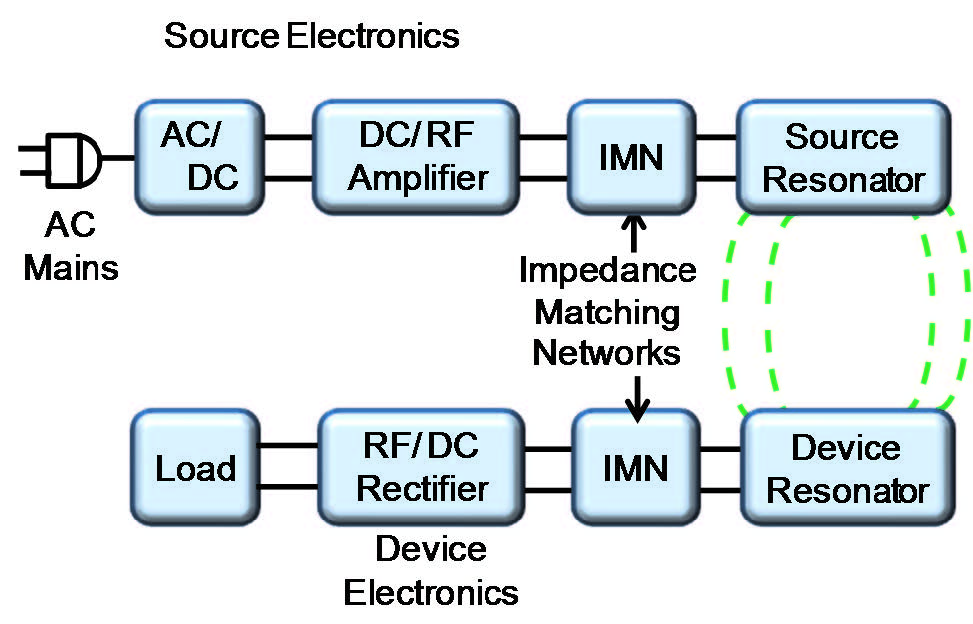
\includegraphics[width=0.85\textwidth]{lit-review/witricity-schematic}
    \caption[WiTricity schematic]{Schematic of WiTricity's HRMC System~\cite{kesler_highly_2013}}
    \label{fig:lit-review-witricity-schematic}
\end{figure}

HRMC uses magnetic induction to transmit energy between two coupled antennas. HRMC continually adjusts the coupling of transmitter and receiver antennas to keep both at a mutual resonant frequency. This technique, impedance matching, minimizes the amount of wave reflection inside the transmitter and receiver circuits, maximizing the energy passed to the load component. This process requires a continuous proprietary feedback mechanism to optimize the receiver for the given distance from the transmitter.

WiTricity has demonstrated that the range of HRMC can be increased through the use of coupled relays. These relays can be coupled with the transmitter, allowing the effective range of the transmitter to increase with minimal additional loss~\cite{butler_tour_2013}.

\subsubsection{WattUp}
WattUp's central idea is to use Bluetooth to transfer information about the receiver's location relative to the transmitter, allowing the transmitter to directly focus energy on the receiver~\cite{energouscorporation2016}. Once it has locked in a signal, it may boost the output power from mW RF signals to multiple W RF signals such that the receiver can charge. WattUp highlights two main features of its technology: (1) the range over which \numrange{1}{4}~W may be quickly and safely transmitted and (2) the relatively large number of devices that may be powered at once (currently 12, with 24 being available in the future)~\cite{energouscorporation2016}.

WattUp cites that they may deliver up to 4~W to 4 devices simultaneously within 0-5 feet of the transmitter, 2~W to 4 devices simultaneously within \numrange{5}{10}~feet, and 1~W within \numrange{10}{15}~feet~\cite{energouscorporation2016}. This inverse relationship between delivered power and range is similar to the trend seen with WiTricity, as previously discussed. These numbers only represent the current model and demonstration version of the technology. WattUp claims that for ranges up to 5 feet, the device will charge as if it were plugged into a wall outlet, for 5-10 feet, the device will resemble USB port charging from a computer, and for \numrange{10}{15}~feet users can still power up at slower charge rates. Based on the aforementioned values provided by WattUp, the overall max range is about 15 feet with a max output power of about 10 W, although these two conditions may not be met at the same time.

The technology itself uses two separate RF frequencies to perform wireless charging, representing both the Bluetooth communication (2.4~GHz) and power transfer frequency (5.7~GHz)~\cite{energouscorporation2016}. Both of these frequencies are allowed unlicensed frequency bands that are known to be used for wireless communication. We believe that WattUp chose to use separate frequencies in order to more easily differentiate the signals used for either targeting or power transfer. As the targeting algorithm is proprietary, we are unable to comment on their exact methodology for targeting the receiver.

\subsubsection{uBeam}
The final primary medium range WPT titled uBeam uses an entirely unique method compared to other companies and methods, relying on ultrasonic waves rather than electromagnetic waves~\cite{constine_ubeam_2015}. One can imagine their system as an extremely high power microphone and speaker combination that specifically sends the sound to a device location. Although uBeam is unique in its approach, it boasts comparable range and power levels when discussed next to other WPT companies.

The first difficulty of using sound waves as opposed  to electromagnetic waves is the inherent dissipative nature of air as a medium. Due to this characteristic, uBeam uses output sound levels of \numrange{145}{155}~dB (316 - 3000~$\frac{W}{m^2}$), comparable to the sound produced by a jet engine or shotgun blast ~\cite{galencarolaudio207}. In order for this level of sound to be used safely, uBeam transmission frequencies of \numrange{45}{75}~kHz, as this is far above the audible range of both humans and animals. As an extra safety measure, uBeam cites that ``if a person were to be exposed to the uBeam ultrasound source, 99.9\% of the emitted ultrasound will bounce off the skin''~\cite{constine_ubeam_2015}. These considerations have allowed uBeam to stay well within the FCC safety regulations.
uBeam uses a phased array transmitter with thousands of antennas that result in a power range of \numrange{1}{4}~m. Although the tracking and targeting algorithm is proprietary in nature, uBeam claims the ability to maintain power transfer while the receiver is moving, although uBeam does not cite specific speeds. The technology requires few obstructions in order to work due to the nature of sound as a mechanical oscillation. For example, if a cell phone is in a user's pocket, then it will not be able to be powered as the user's clothing will block or extremely dampen the ultrasonic waves.

As their product has not yet hit the market, numbers for uBeam's efficiency are not available. We do know that the power output from the transmitter is \numrange{145}{155}~dB ~\cite{constine_ubeam_2015}, while a reasonable output at the receiver is on the order of \numrange{1}{10}~ watts. Based on this, the technique seems unlikely to have a high wall-to-load efficiency.

\subsection{Long Range}

\subsubsection{Cota}

Cota uses concentrated microwaves to create ``pockets of energy'' at precise locations. The power-seeking device sends out pulses regularly, which, when picked up by a Cota system, trigger the system to send out a high energy pulse targeted specifically to the device's location.

The Cota system consists of two parts: a charger and a receiver. The Cota receivers built into devices and batteries regularly send out omnidirectional beacon signals. Once the Cota charger receives these beacons, it returns thousands of targeted signals that build hotspots of energy at only the precise locations of the beacons' locations. The charger uses 20,000 antennas to determine the exact direction the signal came from. This pinpoint precision targeting of energy safely and efficiently powers all Cota-equipped devices and batteries within its effective radius, even as they move around the room.

The technology has achieved a 30~ft range and a max power delivery of about 1~W, offering a comfortable operating radius and charging speed at about one-third the charging time via regular USB cable. It also cites the capability to charge as many devices as desired. It does use Bluetooth to link the charger to the receiver(s), which requires that the power-seeking device constantly pulse to request power. This means that charging the device is contingent on the device already having enough power to send that request.

\subsubsection{Wi-Charge}

\begin{figure}
\centering
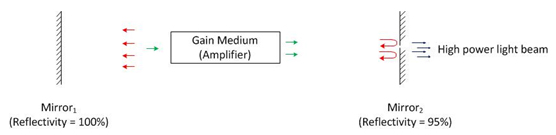
\includegraphics[width=0.85\textwidth]{lit-review/wicharge-1}
    \caption[Wi-Charge: Typical laser]{The resonating chamber of a typical laser. The gain medium allows for stimualted emission of photons. The 95\% reflective mirror partially transmits light, which is observed as the output of the laser~\cite{wicharge2016}.}
    \label{fig:lit-review-wicharge-1}

\vspace*{\floatsep}% http://tex.stackexchange.com/q/26521/5764

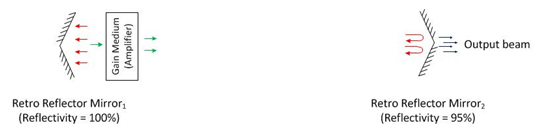
\includegraphics[width=0.85\textwidth]{lit-review/wicharge-2}
    \caption[Wi-Charge: Modified resonating cavity]{A modification of the traditional laser resonating cavity to allow for collimation and coherency of the stimulated photons~\cite{wicharge2016}.}
    \label{fig:lit-review-wicharge-2}

\vspace*{\floatsep}% http://tex.stackexchange.com/q/26521/5764

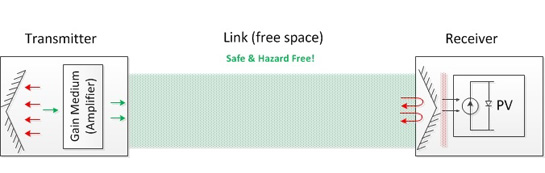
\includegraphics[width=0.85\textwidth]{lit-review/wicharge-3}
    \caption[Wi-Charge: Wi-Charge setup]{The setup of the Wi-Charge system. The fully reflective mirror is on the transmitter, while the 95\% reflective mirror is located within the receiver device. Behind the receiver's mirror is a photovoltaic cell to convert the light back into an electrical signal to power a battery~\cite{wicharge2016}.}
    \label{fig:lit-review-wicharge-3}
\end{figure}

Also capable of a 30~ft operating radius, Wi-Charge uses a combination of a laser cavity and a photovoltaic cell to create robust power transfer systems~\cite{wicharge2016}. To understand the system, it is necessary to discuss how a laser works. Consider Figure~\ref{fig:lit-review-wicharge-1}, which depicts two mirrors and an amplifier between them. Simply put, one photon, an energetic light particle, enters the amplifier and two come out. When the photons hit the mirror, they bounce back through amplifier in the opposite direction and two photons become four. This process repeats with each ricochet against a mirror, and the energy amplifies within the system. This process of recirculating light in a positive feedback loop with an amplifier creates a resonator.

When that resonator has one mirror that is very slightly transparent, as in Figure~\ref{fig:lit-review-wicharge-1}, then a focused, high powered beam is generated. This is a laser beam.

Any particles that do not travel along the axis between the two mirrors will hit the mirror at an odd angle and bounce out of the resonator. This is why only the photons that are traveling in the direction of the axis between the two mirrors will continue to amplify.

Wi-Charge took this traditional definition of a laser, and made a few clever modifications to better suit their purposes, shown in Figure~\ref{fig:lit-review-wicharge-2}~\cite{wicharge2016}.

First, they kept the components--two mirrors with an amplifier between them--but modified their arrangement. Second, they made the mirrors retro-reflectors which, unlike regular mirrors, reflect light back to their sources. The result is that the two mirrors spontaneously form a resonator when placed within each other's \los{}, although the resonator is stalled immediately when the \los{} is broken. This last property may actually be desireable in a consumer setting, as it helps to prevent energy from accumulating anywhere but the intended receiver.

In Wi-Charge's setup, one mirror and the amplifier are grouped together as the transmitter, and a second mirror and a photovoltaic cell are grouped together as the receiver. This is shown in Figure~\ref{fig:lit-review-wicharge-3}. By placing the photovoltaic cell directly after the laser output location, the Wi-Charge system effectively converts the optical signal back to an electrical signal that can be used to charge a battery.

Wi-Charge is a long range wireless power solution that can deliver up to 10~W of power~\cite{wicharge2016}. It can latch onto targets almost instantaneously and cease beaming equally quickly, intrinsically. It can also power multiple devices. However, the system does require \los{}.

\section{Time Reversal}
\label{lit-review-tr}

\subsection{Conceptual Overview of Time Reversal}

The lossless wave equation is time-reversal invariant: for any normally propagating wave taken to be a time-forward solution, there is a corresponding time-reversed solution representing that wave traveling in the opposite direction. The technique known as time reversal (TR) exploits this property of waves to focus a signal onto the point of origin of some other, previous signal. TR can locate objects without prior knowledge of their position or their surrounding geometry.

A system that performs TR is called a ``time reversal mirror'' (TRM), sometimes simply shortened to ``mirror.'' A TRM consists of one or more transmitters to introduce waves into a chamber and one or more receivers to record the echoes from it. The transmitters and receivers may (but do not have to be) the same device. TR requires an at least partially echoic chamber that allows waves to reflect off of its interior geometry and return to the transmitters. Here we refer to such a chamber as ``reverberant''.

\begin{figure}
    \centering
    \begin{subfigure}{.85\textwidth}
        \centering
        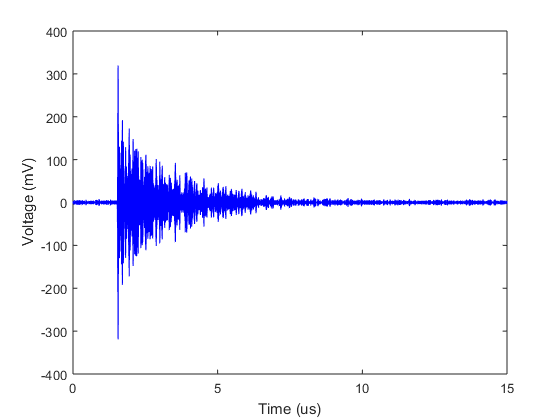
\includegraphics[width=0.9\linewidth]{lit-review/example-sona}
        \caption[Example sona]{Example sona}
         \label{fig:lit-review-example-sona}
    \end{subfigure}
		\par\bigskip
    \begin{subfigure}{.85\textwidth}
        \centering
        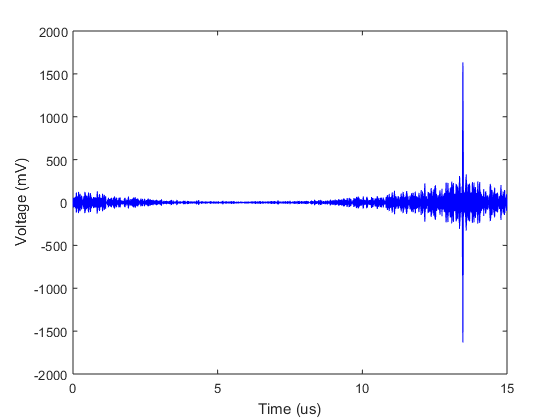
\includegraphics[width=0.9\linewidth]{lit-review/example-recon}
        \caption[Example reconstruction]{Example reconstruction}
         \label{fig:lit-review-example-recon}
    \end{subfigure}
    \caption{Recorded sona and reconstruction from a typical TRM experiment}
    \label{fig:lit-review-example}
\end{figure}

A TRM works by broadcasting a waveform into the reverberant chamber and recording the resultant echo. This echo will consist of many time-shifted overlays of the original waveform. We refer to this echo as a ``sona'' in this thesis. An example sona is shown in Figure~\ref{fig:lit-review-example-sona}. The sona is time reversed and rebroadcast, which will cause the waves to trace their paths in reverse and return to their source in a semi-coherent ``reconstruction'' of the original broadcast. An example reconstruction is shown in Figure~\ref{fig:lit-review-example-recon}: in this case, the original signal was a short pulse in the same shape as the large vertical spike near the right of the figure. Since it involves waves from many scattered paths all suddenly arriving at the same point, reconstruction is also known as ``collapse.''

TR is relatively versatile. If the technique is iterated exactly as described, the broadcasts will collapse more and more exactly on the strongest scatterer in the chamber~\cite{fink_time-reversed_1999}. Many other methods can be used to select targets more discriminately, and the generic TRM itself can be modified as well -- for example, by recording directly from a target position, it is possible to create a secure channel between that point and the transmitter~\cite{nltr-wave-chaotic}.

\subsection{History of Time Reversal Research}

TR is a proven technique in signal processing, with applications in acoustics as well as electromagnetics. Though its publicity is limited, there is a wealth of available literature regarding TR in certain specialized areas. Here we briefly describe the development and historical applications of the technique to illustrate where TESLA's project will expand this literature.

Time reversal as a technique was first developed in the 1990s. Some of the earliest and most influential work was conducted through teams led by Mathias Fink and Claire Prada of the University of Paris. These researchers used the technique to focus sound waves on ``scatterers,'' objects that reflect the pulses~\cite{prada_iterative_1991}. An array of transducers would fire a sonic pulse into some propagation medium and listen for the echo. The recording of that echo was reversed in the time domain and transmitted back into the medium. They repeated (iterated) this process, causing the acoustic signature of the strongest scatterer to appear more prominently each time. In this way, the team was able to iteratively focus on the scatterers without needing prior knowledge of their location. Prada and her team submitted this DORT (French acronym, English: Decomposition of the Time Reversal Operator) method as a process for finding cracks or faults in structural members~\cite{prada_iterative_1991}. More importantly, Prada et al. went on to demonstrate that the method could always resolve the brightest scatterer if given enough iterations, that it worked better in a heterogeneous medium than a homogenous one, and that it was both experimentally and mathematically possible to resolve multiple targets at once~\cite{prada_decomposition_1996}. These discoveries generated significant interest in a subset of the acoustics research community.

Others in the field of acoustics went on to refine the DORT method as an imaging technique, and as the field gathered attention, further explored formalizing the problem in general. An excellent example of the latter is the theoretical work by D. H. Chamber in his 2007 examination of TR for target detection and characterization~\cite{chambers_target_2007}. In 2010, Nguyen and Gan developed a way to extract much more information from an anisotropic (directionally distinct) scatterer, including its rough shape, density, and radius. In doing so, they developed a faster mathematical approach to locating their scatterers that relied on several good approximations instead of one exhaustive computation~\cite{nguyen_dort_2010}. Also in 2010, Barbieri and Meo made a large contribution to the field by bringing together the DORT method, which works in linear environments, and another similar method for working in nonlinear environments. This allowed them to resolve and distinguish between linear scatterers such as holes and nonlinear scatterers such as cracks~\cite{barbieri_time_2010}.

Imaging is not the only application for a focusing method, however, and others adapted the existing body of TR research to new problems. The reciprocity of the wave function that Fink and Prada relied on to develop the technique holds for all waves it can be used to model. This means that the time-reversal operation works much the same way with electromagnetic waves as it does with sound waves~\cite{chambers_target_2007}. This was explored as early as 1999, but was largely concerned with the same imaging problems occupying those in acoustics until at least 2007~\cite{chambers_target_2007}. However, that gradually began to change. In 2011, a team including graduate students from the University of Maryland posited that time reversal was an ideal mechanism for wireless communication~\cite{wang_green_2011}. In the same way that a sound wave could be made to collapse on a scatterer, they showed that an information packet could be made to collapse on a receiver. The team submitted this as an eco-friendly communication method because information transfer could be accomplished using less energy~\cite{wang_green_2011}. Later, this same property was examined for its security benefits instead of its environmental ones. In February of 2013, a team of researchers at the University of Maryland, including Matthew Frazier and Steven Anlage, published a study discussing TR as a method to selectively send information in a chaotic wave environment~\cite{nltr-wave-chaotic,taddese_sensing_2010}. The team was able to create an exclusive communication link to a certain object, without needing to know its location and without interfering with nearby objects. In their experiment, they were able to transmit data (in the form of images) exclusively to a desired port, while the other port received only garbled noise.

Beyond its practical applications, in the process, Frazier and his team used nonlinear elements to extend TR in new and exciting ways. Recall that in traditional TR many iterations are required to pinpoint the target. The addition of a significantly nonlinear element greatly simplifies the pinpointing process. When a wave strikes the element, harmonic frequencies are produced at integer multiples of the original frequency. These harmonics can be quickly located in the echo's frequency domain and filtered in order to select them exclusively. The important distinction is that since the harmonics originated directly from the target antenna, all subsequent broadcasts of the TR signal will collapse on the antenna without the need for iteration~\cite{nltr-wave-chaotic}. Frazier and the others put forth several exciting directions to pursue with this concept: the secure communication channels mentioned above, hyperthermic treatment of tumors, and a long range WPT system that eschews traditional high power beams. It is this last area that TESLA intends to explore.

\chapter{Linear Time Reversal}
\label{ch:ltr}

\section{Purpose}
\label{sec:ltr-purpose}

In investigating the applicability of time reversal to a wireless power transfer system, there are several properties that we would like to characterize further. While transferring a meaningful amount of energy to a receiver is the primary goal, but there are other characteristics to consider as well. We are interested in the ability to select a receiver to send energy to, while minimizing the wasted energy that is sent to other locations. We are interested in being able to transmit energy to a receiver in a complex environment, which may have an obstructed line of sight. We are interested in transferring power to a receiver in motion. How does TR perform in these capabilities?

The following sections detail the research that TESLA has done in the field of TR WPT. These experiments are meant to accomplish several goals:

\begin{itemize}
    \item Characterize the behaviors of TR relevant to WPT applications
    \item Understand fundamental limitations of TR applied to WPT
    \item Create a baseline for which future work can be done
\end{itemize}

The general methodology for the experiments is described. Then, the purpose, methodology, and results of individual experiments are discussed individually.

\section{Methodology for Conducting Linear Time Reversal Measurements}
\label{sec:ltr-meth}

The majority of our experiments take place within an enclosed, reflective cavity called the Gigabox: an aluminum box with a metallic foil scattering paddle to make the ray trajectories more ergodic. Ray chaos ensures that a propagating pulse will eventually reach every point in the environment. This improves reconstruction fidelity. Up to five monopole antennas inject and extract electromagnetic signals from different ports in the enclosure depending on the experiment.

Our Time Reversal scheme consists of three pieces of microwave processing equipment and a desktop workstation. Interrogation pulses and time-reversed sona signals are created and broadcast using a Tektronix \texttt{AWG7052} arbitrary waveform generator feeding an Agilent \texttt{E8267D} Vector PSG microwave source. A digital storage oscilloscope (DSO, Agilent \texttt{DSO91304A}) is used to record waveforms of interest. MATLAB is used for signal processing and instrument control and coordination.

In many experiments, it is necessary to be able to ``read'' and ``write'' signals from the same port. Manually switching coaxial cables from the PSG to the DSO is slow and can destroy reconstructions, so we use four HP 8762C coaxial switches to reroute signals as required.

This hardware is laid out in Figure~\ref{fig:linear-gigabox}.

\begin{figure}[h!]
\centering
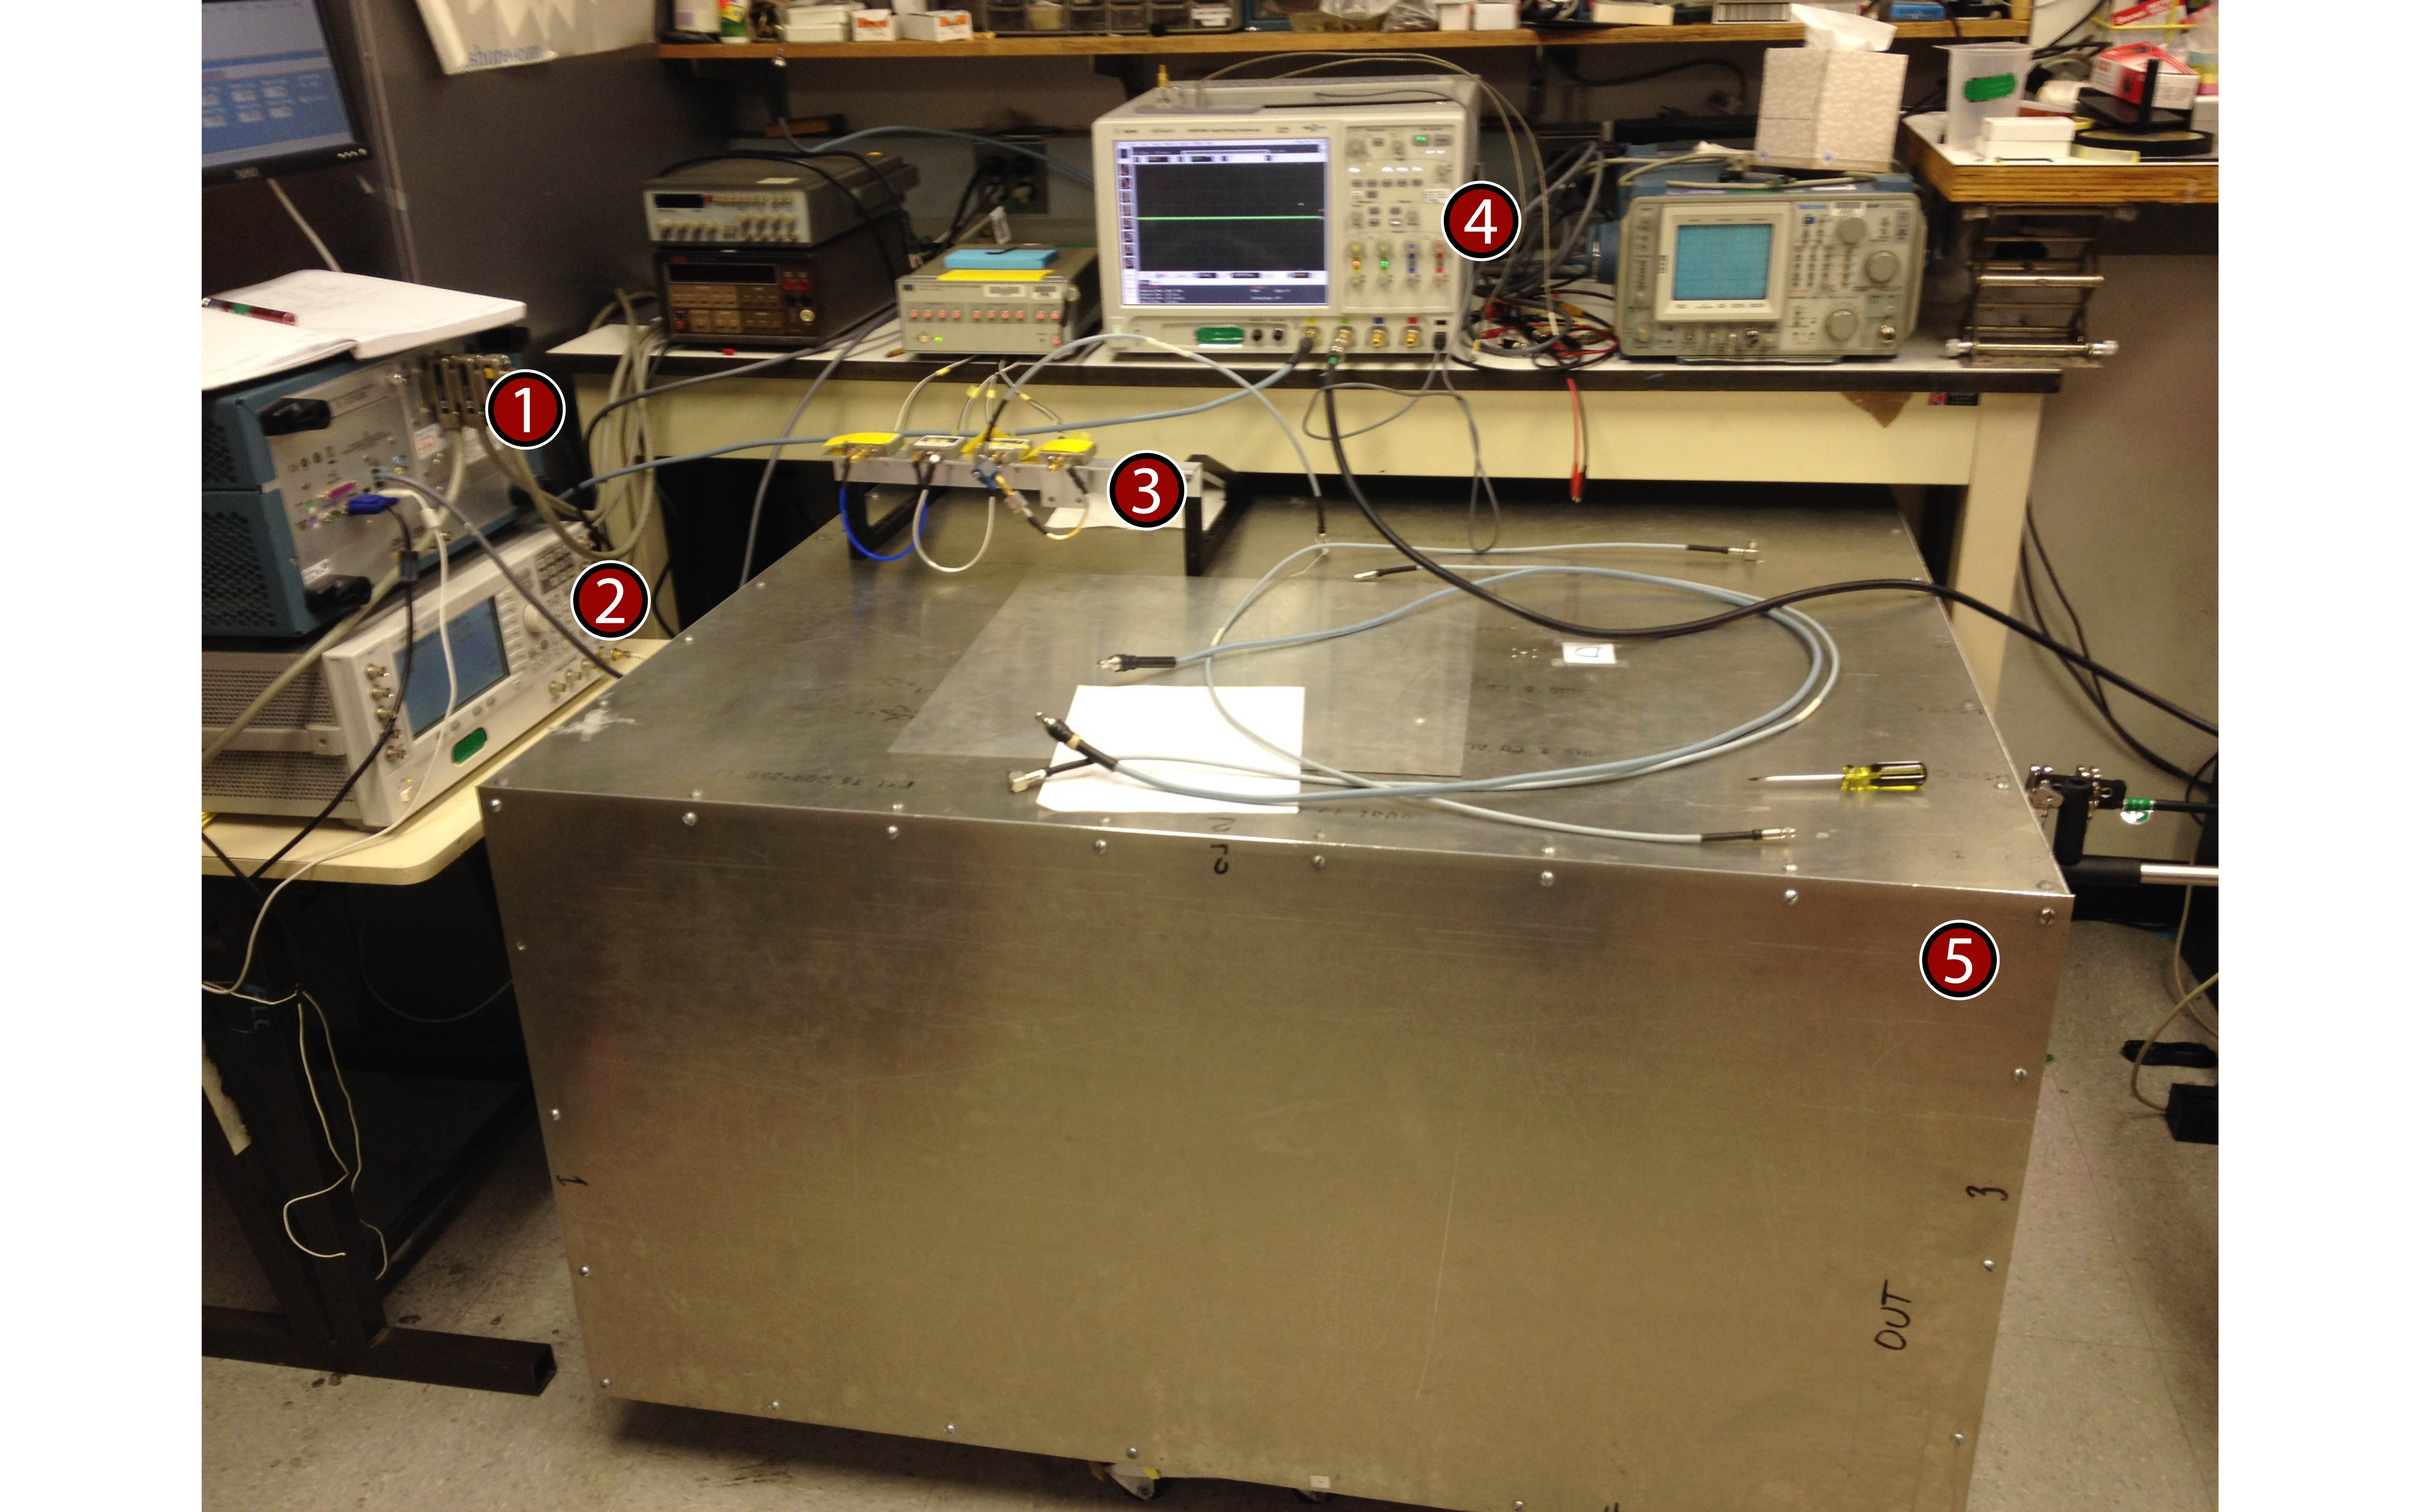
\includegraphics[width=0.85\textwidth]{linear/gigabox}
    \caption[Lab equipment setup]{Lab equipment setup: (1) Tektronix \texttt{AWG7052} Arbitrary Waveform Generator, (2) Agilent \texttt{E8267D} Vector PSG Microwave Source, (3) Array of four Hewlett-Packard 8762C coaxial switches, (4) Agilent \texttt{DSO91304A} Digital Storage Oscilloscope, 5) 1.06~$m^3$ aluminum ``Gigabox'' with interior conductive scattering paddle.}
    \label{fig:linear-gigabox}
\end{figure}

Our TR experiments fall into two main categories, linear and nonlinear. Linear TR (LTR) refers to any experiment that uses a single frequency. Nonlinear TR (NLTR) makes use of harmonic reflections from the target to provide a means for isolation and targeting, a process similar to how we would envision a TR based WPT system to work.  It is experimentally much simpler to create reconstructions with LTR than with NLTR, so we use it for experiments investigating the behavior of the waves rather than the behavior of the target.

This section concerns LTR experiments. Conceptually, our general process for LTR in the Gigabox is as follows: we broadcast a Gaussian interrogation pulse from one port, serving as a transmitter. This interrogation pulse reverberates and echoes around the reflective cavity. Another port, designated as the receiver, records the multipath sum of these reverberations with the oscilloscope. This summed signal is named a sona, and inherently contains information relating to the size and shape of the interrogation pulse, the location of any scattering media in the environment, and the location of both ports. That sona is reversed in the time domain and subsequently rebroadcast from the transmitting port. The signal will travel through the same multipath channels and reconstruct a time reversed version of the original interrogation pulse upon the receiver, with some additional noise. This process is illustrated in Figure~\ref{fig:linear-ltr}.

\begin{figure}[h!]
\centering
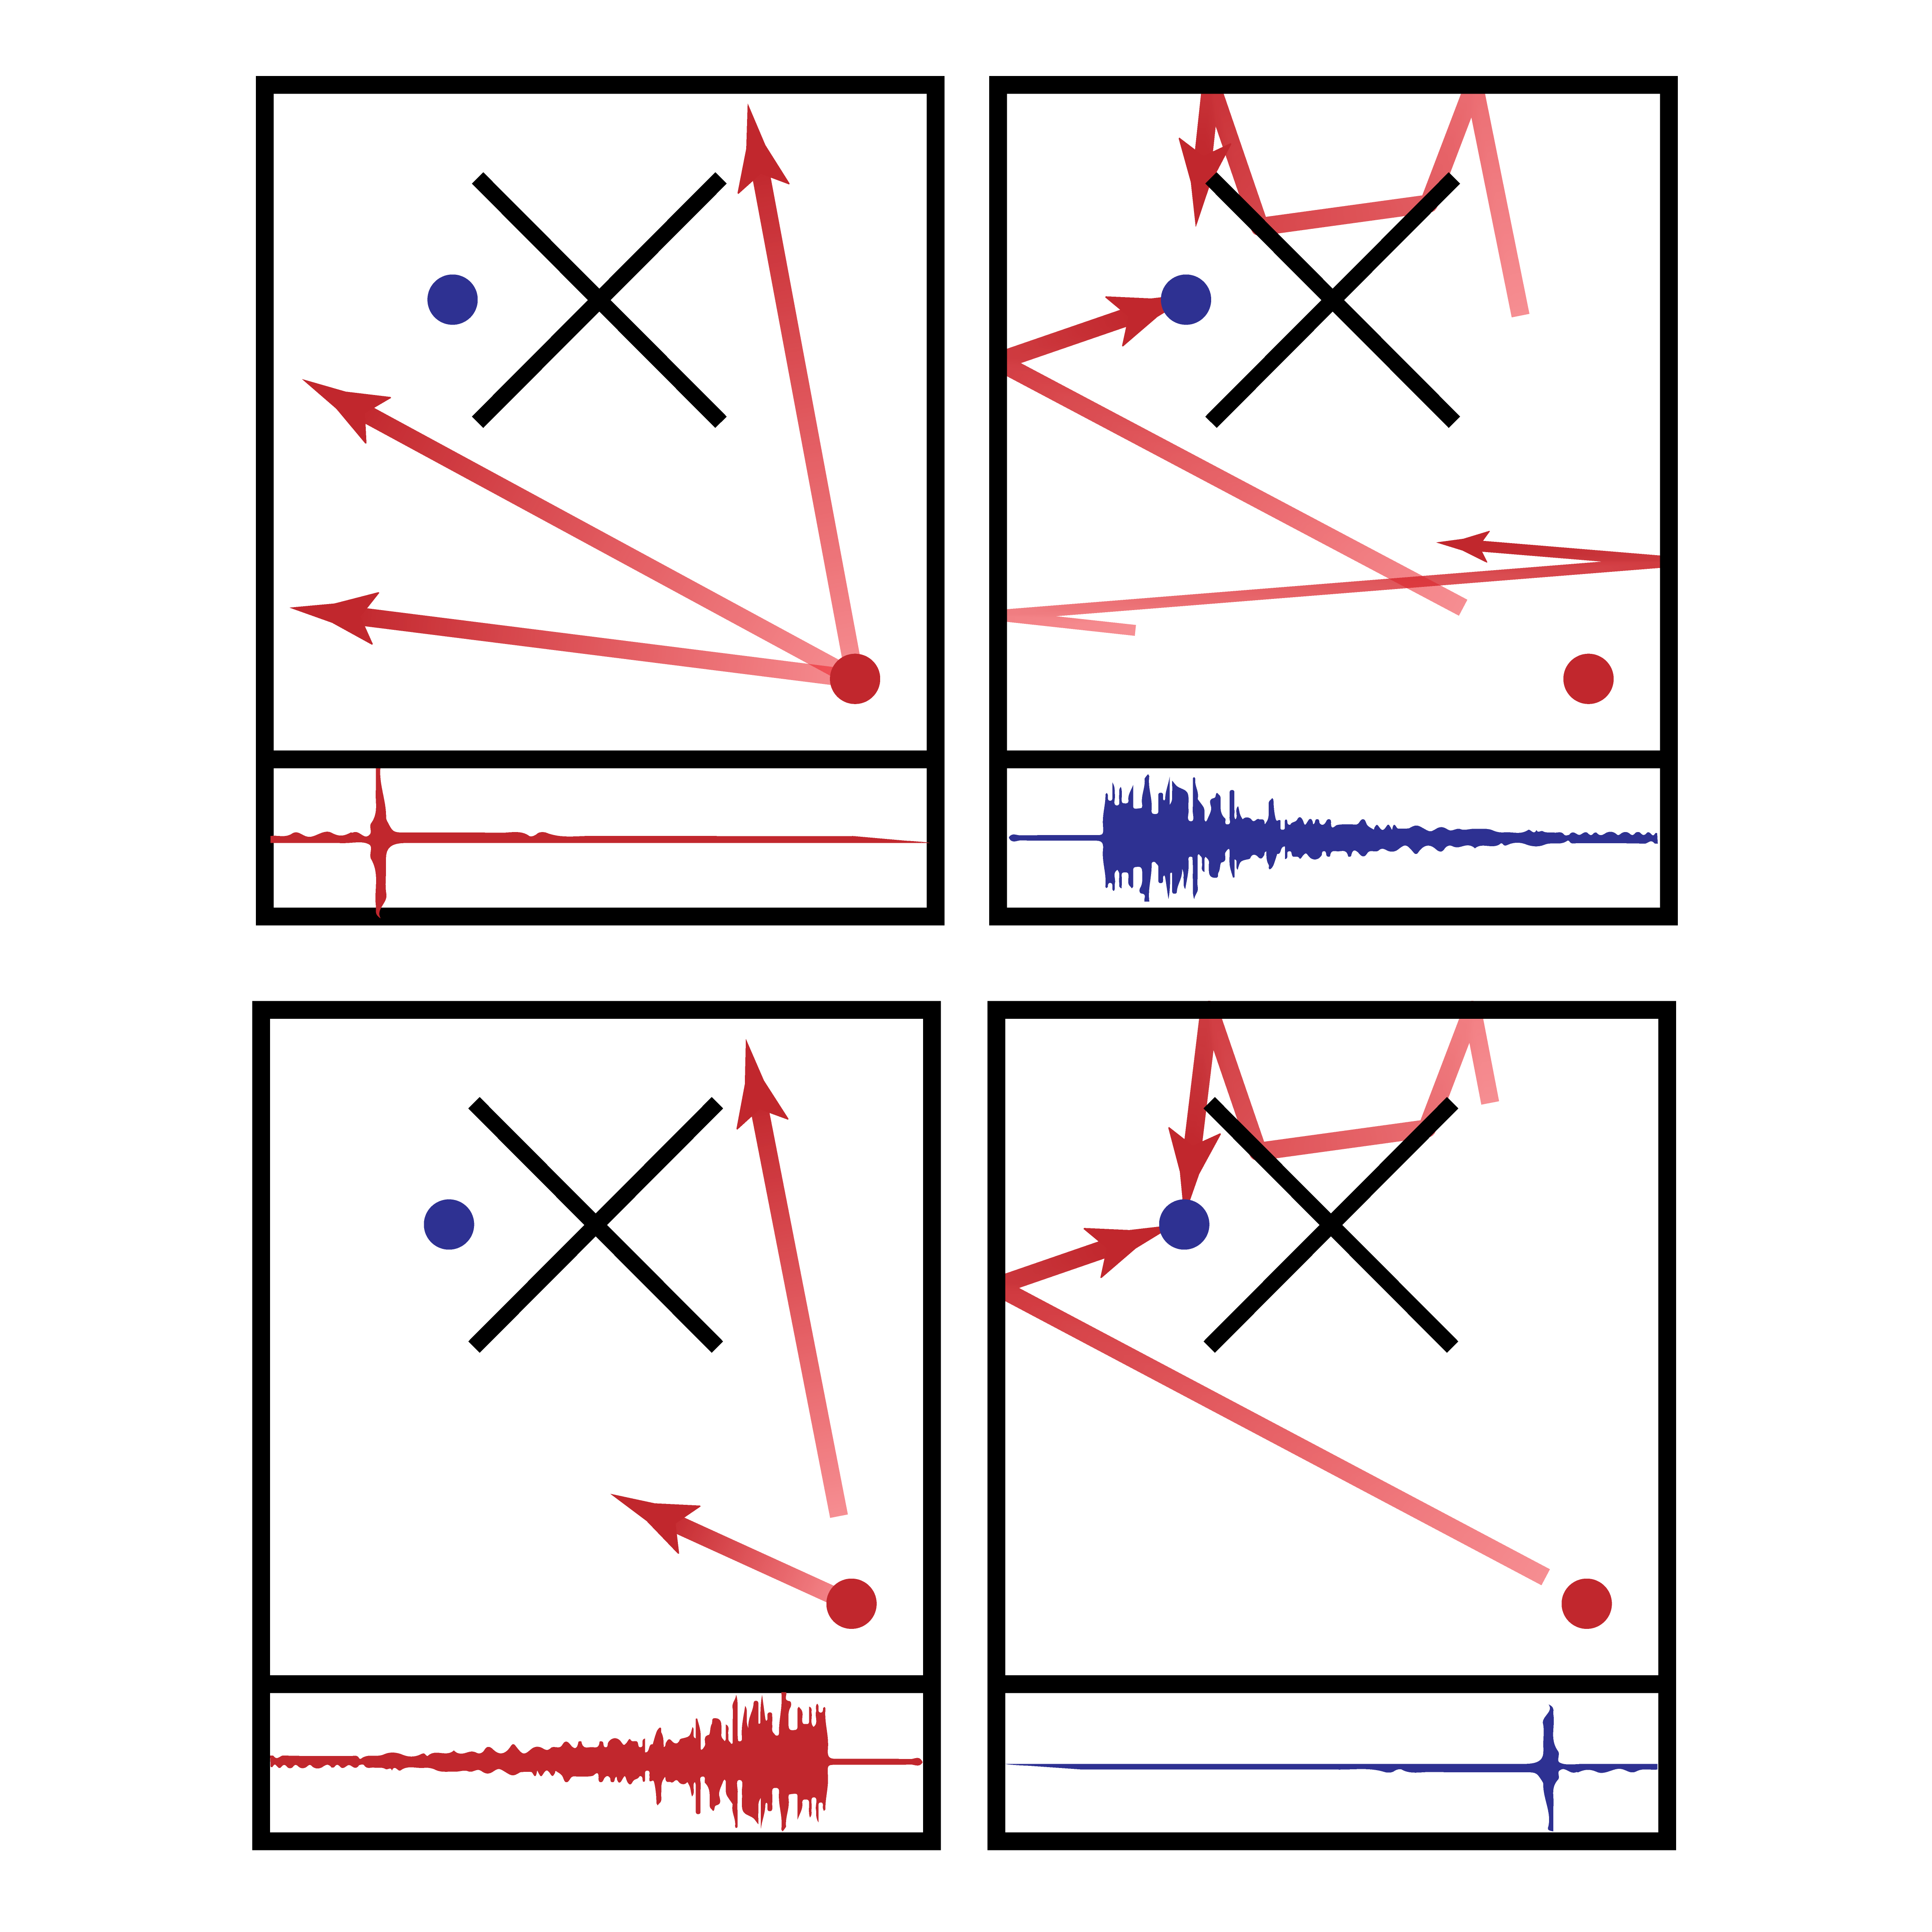
\includegraphics[width=0.85\textwidth]{linear/ltr}
    \caption[Conceptual overview of linear time reversal]{Reading order from top left: Visualization of the linear time reversal process (1) The TRM broadcasts a signal (in this case,a pulse, pictured in the inset below the panel) into the cavity, which (2) reverberates within the cavity. Some of the reflections incoherently reach the receiver as the sona, represented in blue in the inset. (3) The TRM time reverses the sona, then re-emits it into the cavity. (4) The time reversed waves coherently collapse back on the receiver in a slightly distorted reconstruction of the original pulse (inset, blue).}
    \label{fig:linear-ltr}
\end{figure}

Since this LTR process is well-suited to creating reconstructions of Gaussian waveforms, we used it for three experiments to examine characteristics and modifications of LTR itself. These were: 
\begin{itemize}
    \item Overlaying sonas to create more reconstructions closely spaced in time
    \item Mapping the spatial profile of a reconstruction
    \item Repeatedly retargeting the reconstructions upon a moving antenna
\end{itemize}
The experiments, results, and discussions for these sections are presented respectively as "Overlapping Reconstructions", "Spatial Profiling", and "Moving Reconstructions" below. The experience the team gained by performing these experiments and formulating results was invaluable in constructing and performing our later work with Nonlinear Time Reversal (NLTR). They also demonstrate important ideas regarding the transmission of large amounts of power to the receiver.

\section{Overlapping Reconstructions}
\label{sec:overlapping}

\subsection{Purpose}

Frazier et al. demonstrate that the sona of a given interrogation pulse is significantly longer than the pulse that generated it~\cite{nltr-wave-chaotic}. This stands to reason, given that the sona represents reflections of the initial pulse shifted in time by differing path lengths.

To start with, an important feature of this method is spatial fidelity: the ability to deliver highly localized reconstruction to a reciever. In the interest of delivering more energy with each packet, there is a desire to make the duration of the reconstruction longer. To do this, however, would reduce the bandwidth of the interrogation pulse and reconstruction. The bandwidth of the interrogation pulse translates to the number of eigenmodes available for comunication between the transmitter and reciever. The requirement for a suitibly large bandwidth restricts the duration or temporal localization of the interrogation pulse and reconstruction. As a result, increasing the energy delivered per reconstruction packet by extending the duration of the interrogation pulse is not a favorable option as it reduces the spatial fidelity of the reconstruction.

To increase the amount of energy transmitted, we propose two modifications to the time reversal scheme. Either the amount of energy contained within each packet can be inflated, or the frequency of packets can be increased. Increasing the size of the reconstruction is a trivial matter; by amplifying the time reversed sona before reinjection, the reconstruction is correspondingly amplified. We desire to send reconstructions more frequently than the length of the sona will allow. However, transmitting multiple sonas at once from the same antenna is possible--copying and shifting the signal in time can allow several signals to be sent in less time than the sum of the individual sona time lengths. This will in turn result in multiple transmitted reconstructions, and improved power transmission.

A concern with the above method is whether or not it would result in lost information and consequently degraded reconstruction quality. Sonas are sinusoidal signals--if overlaid, they will interfere constructively and destructively. Destructive interference may result in the ``deletion'' of transmission paths, reducing the efficiency of the TR process and decreasing the fidelity of the created reconstructions. In this experiment, we are interested in understanding the degree to which superimposing sonas will degrade the ability to transmit energy between ports using linear time reversal.

\subsection{Methodology}

This test sought to evaluate the practicality of overlapping sonas as a method of transmitting power. This experiment was done using the basic, two-port linear time reversal scheme, first described in Section~\ref{sec:ltr-meth}. A diagram of this scheme appears as ~\fig{ltr-process}.

\begin{figure}[h!]
\centering
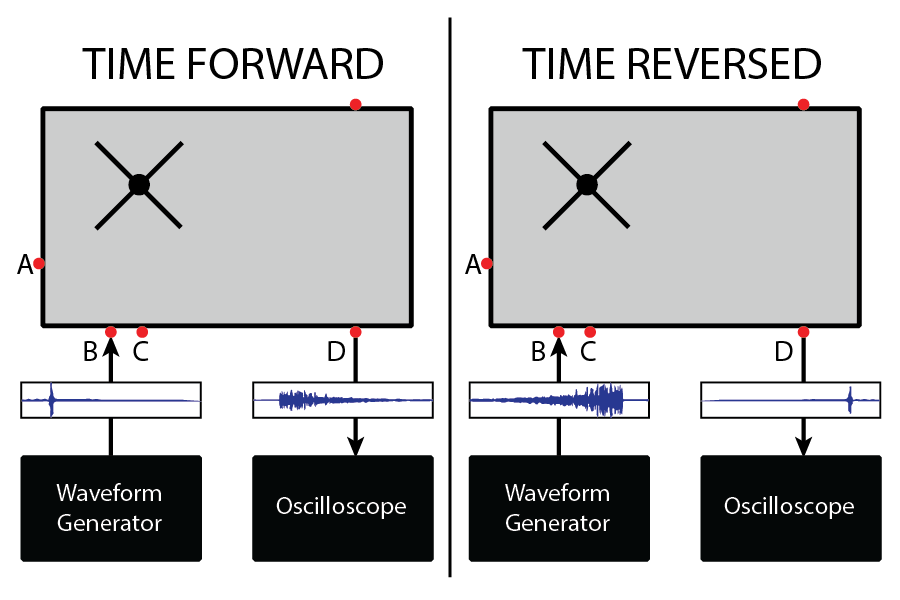
\includegraphics[width=0.85\textwidth]{linear/ltr-process}
    \caption[Two-Port Linear Time Reversal Setup]{A diagram of our typical two-port linear time reversal scheme. In the time forward step, a pulse is broadcast from antenna port B and a sona collected at D. In the time reversed step, the reversed sona is broadcast from B and a reconstruction occurs at D. This setup takes advantage of spatial as well as temporal reciprocity to avoid having to record and broadcast from the same port, which greatly complicates cabling and introduces losses from the switches.}
    \label{fig:ltr-process}
\end{figure}

A sona was generated with a 3.9 GHz interrogation pulse. To verify that the sona could converge on the target, it was time reversed without any further manipulation, and injected back into the cavity. The reconstruction was recorded and compared to the original interrogation pulse to check for irregularities.

Once the efficacy of the single sona was established, the experiment was modified. Several sonas were superimposed with a constant time shift, resulting in evenly spaced copies of the verified sona across the total broadcast window. Figure~\ref{fig:overlapping-sonas} gives an example of sonas overlapping in this way. The resulting signal was then time reversed and broadcast through the linear system in the same manner as before, which resulted in the reconstructions in Figure~\ref{fig:overlapping-recons}. This test was repeated many times, with the number of sonas superimposed within the 15~$\mu$s broadcast window varying from one to three hundred. This corresponds to repetition rates between 66 kHz and 20 MHz.

\begin{figure}
\centering
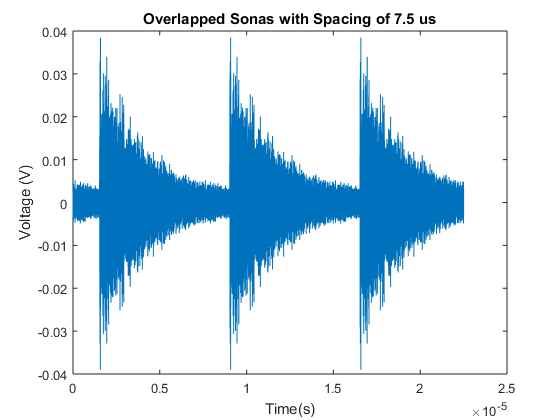
\includegraphics[width=0.85\textwidth]{overlapping/sonas}
\caption[Overlapped sonas]{Overlapped sonas with a spacing of 7.5~$\mu$s.}
\label{fig:overlapping-sonas}

\vspace*{\floatsep}% http://tex.stackexchange.com/q/26521/5764

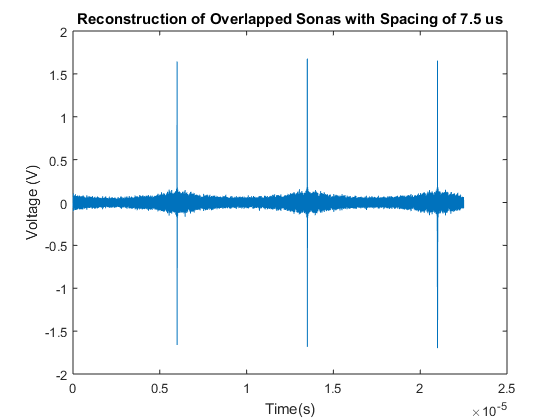
\includegraphics[width=0.85\textwidth]{overlapping/recons}
\caption[Overlapped reconstructions]{Reconstructions resulting from the sonas in~\ref{fig:overlapping-sonas}.}
\label{fig:overlapping-recons}
\end{figure}


\subsection{Results}

Increasing the number of sonas should increase the amount of power transmitted in a given time frame, if the amplitude of each reconstruction remains constant. We hypothesized that overlapping reconstructions by linearly superimposing sonas would not decrease the size of the reconstructions. As a result, a great amount of effective power was transmitted per duty cycle. Our experiments seemed to support this conjecture, in that the number of reconstructions in the cycle could be increased while maintaining their characteristic shape. However, the size of the packets did decrease as the number of reconstructions within the window became larger.

We believe these results to be a combination of two factors. The loss of information due to destructive interference during sona superposition, and the function of power scaling within the PSG signal generator both may have contributed to this decreasing trend. The generator attempts to level a preset amount of power across the entire broadcast window, which is split among the multiple reconstructions.
To better model how these reconstructions would interact with a practical WPT system, we also examined the ``total \ptp{} voltage,'' which we defined as the maximum \ptp{} voltage multiplied by the number of reconstructions present within the measurement window. This quantity emulates the energy that would be rectified within the same time window, so we can compare the various repetition rates with regard to the energy that a receiver would accept within that time frame. This correlation is plotted in Figure~\ref{fig:overlapping-total-voltage}.

Important to note is the overall increasing trend, which resembles a square root function. This is expected, as the power is expected to vary linearly with the number of overlaid sonas, and is proportional to the \ptp{} voltage squared. The positive correlation between repetition rate and total voltage indicates that the use of this technique would be very valuable for a WPT scheme. We can acquire a sona and then broadcast the time reversed version at very high repetition rates to transmit large amounts of energy to the receiver. Coupled with an arbitrary amplification according to the application's needs, this modification to a time reversal WPT system shows promise for increasing the quantity of power that can be transferred.

\begin{figure}
\centering
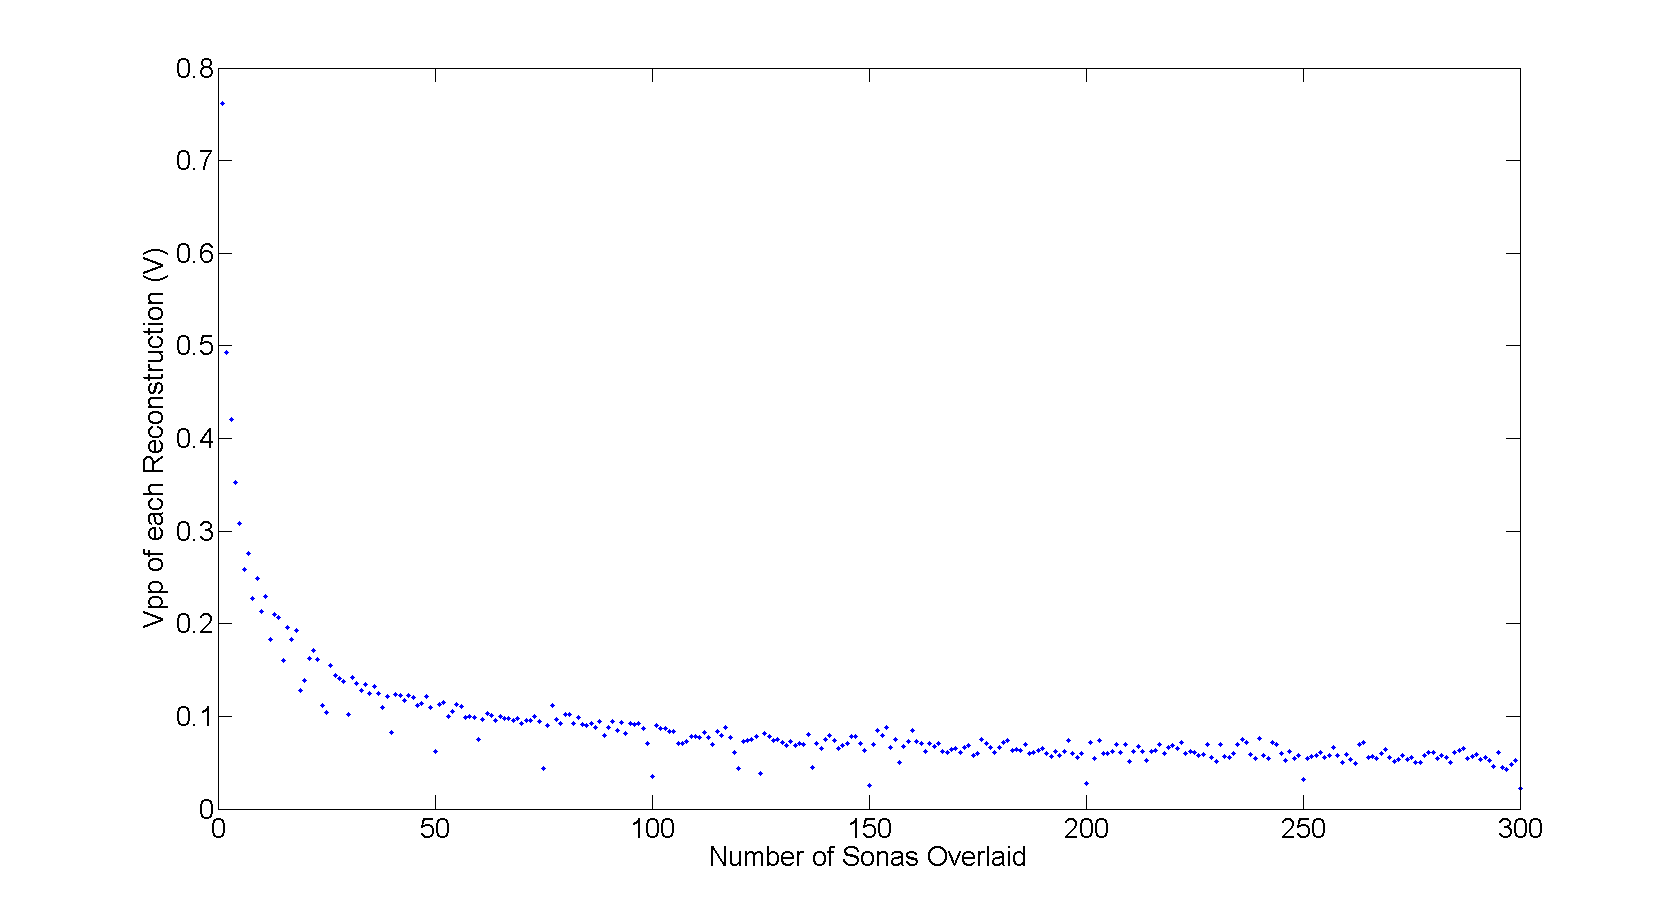
\includegraphics[width=0.85\textwidth]{overlapping/voltage_per_recon}
\caption[Max \ptp{} voltage from overlapped reconstructions]{Max \ptp{} voltage versus number of overlapped reconstructions.}
\label{fig:overlapping-vpp}

\vspace*{\floatsep}% http://tex.stackexchange.com/q/26521/5764

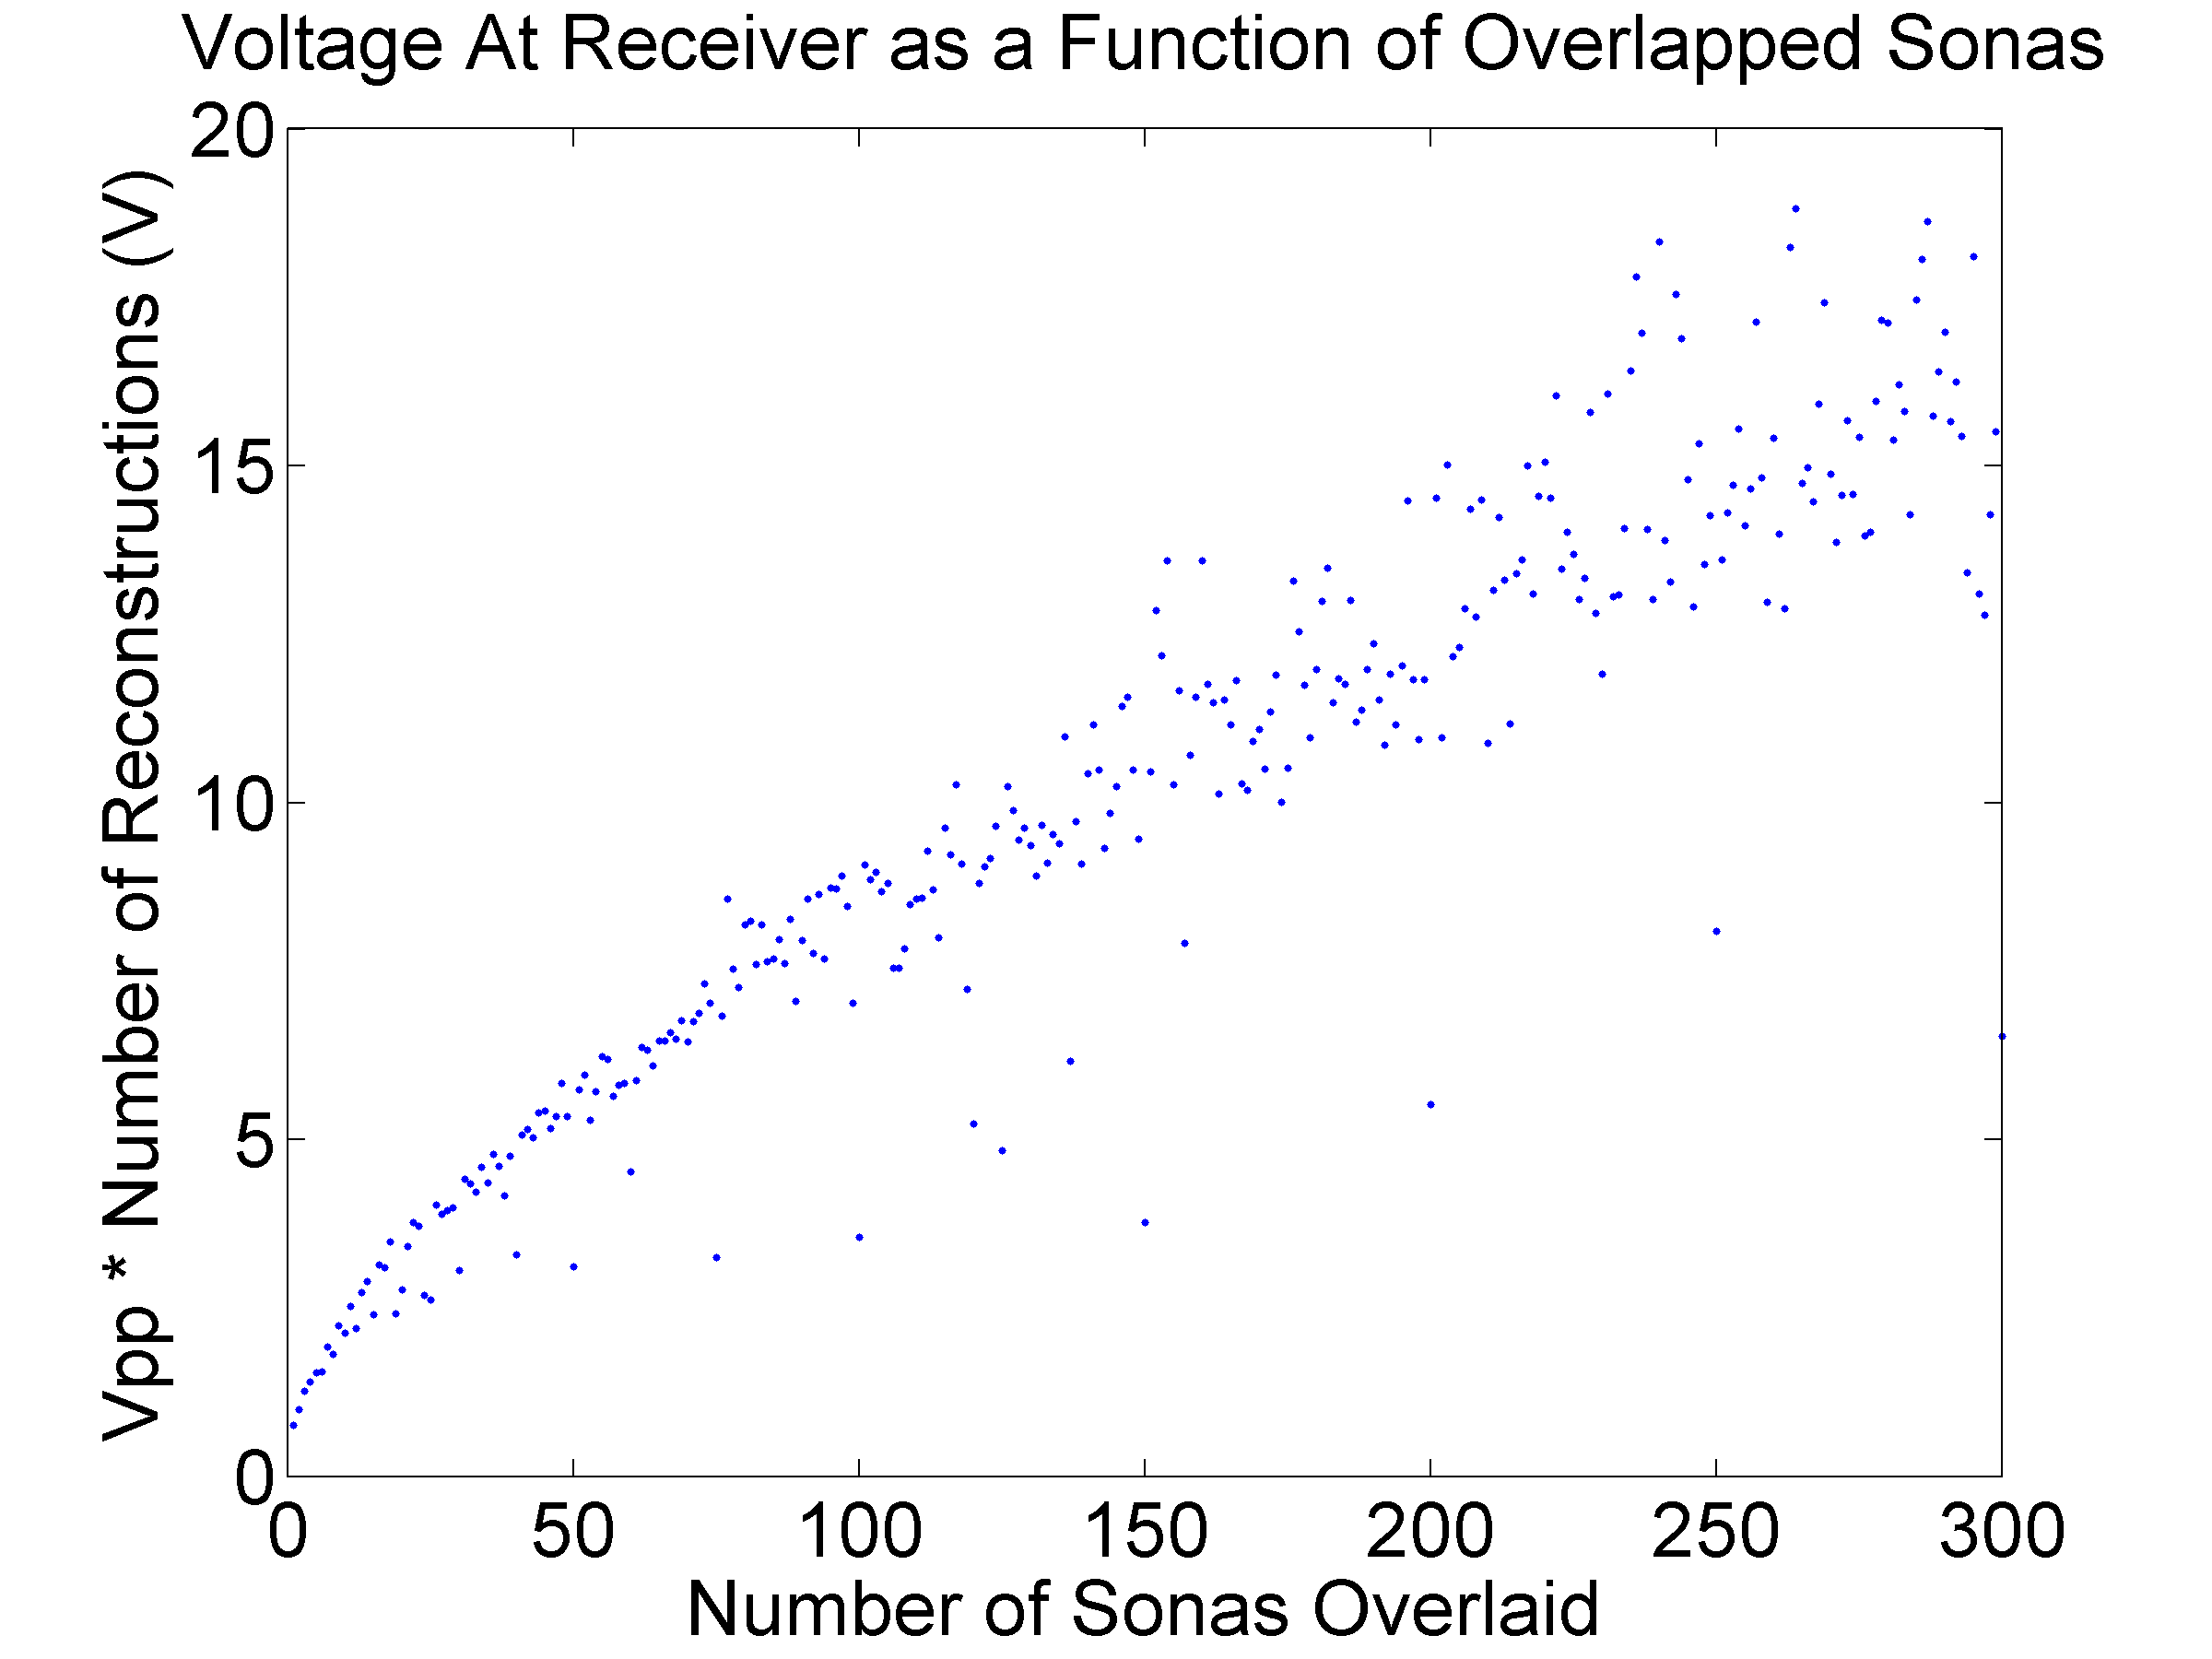
\includegraphics[width=0.85\textwidth]{overlapping/total_voltage}
\caption[Total \ptp{} voltage from overlapped reconstructions]{Total \ptp{} voltage versus number of overlapped reconstructions.}
\label{fig:overlapping-total-voltage}
\end{figure}

\section{Moving Reconstructions}
\label{sec:moving}

\subsection{Purpose}
The TR process assumes that the environment remains fixed between the time-forward and time-reversed steps. It also assumes that the source and target remain fixed between these two steps. However, in a practical WPT system it is desirable to support a receiver in motion. This ability gives a convenient benefit to the consumer, who would not be limited to keeping their mobile device stationary for charging. This is a gap in the current market, which TR may be able to fill. In this section, we propose and investigate a method for using the broad spatial voltage profile to provide a consistent voltage to a receiver in motion.

The experiment is conducted in two parts: mapping the spatial voltage profile of a TR reconstructed signal, and iteratively updating the target location of the time reversal mirror. The first part of the experiment intends to consider the extent to which a reconstruction is localized in space. This property has implications for several parts of the WPT scheme including system efficiency, health concerns, and tolerance in receiver position relative to the target location. A broad reconstruction in space would relate to a lower efficiency, because only a fraction of the energy that is being sent is collected by the receiver. Consequently, if the reconstruction is broad then there is a possibility that some energy could be sent to an unintended nearby medium; for example, the target device might be in a user's pocket, and a broad profile could indicate that the user themself would be absorbing some of that energy. While both of these effects are generally things that we would like to avoid in a WPT system, it also could facilitate the accommodation of a moving receiver. A profile that is not particularly localized would allow the receiver to shift slightly from the target location and still collect a significant portion of the energy packet that was sent. When the voltage level at the receiver's position drops below some acceptable level, the TR process could be performed again. This would update the target location to the receiver's current location, and reset the voltage at the receiver to the peak value of the reconstruction. A broader reconstruction in space would allow this process to be performed less frequently, while a narrower reconstruction may greatly limit the speed that the receiver could travel at.

\subsection{Spatial Profiling}
\label{sec:spatial-profile}
\subsubsection{Methodology}

The setting for this experiment differs only slightly from the one described in Section~\ref{sec:ltr-meth}: now, the receiving antenna is mounted on a PI MikroMove \texttt{M-415.DG} translation stage, shown in Figure~\ref{fig:mikro-move}, which allows the cavity to remain sealed during translation.  Initially, the receiver is moved to the middle of the scanning range (denoted position 0). An interrogation pulse is used to capture a sona and begin creating reconstructions at this initial position. The receiver is then moved from the bottom (-35~mm) to the top (+35~mm) of the scanning range, stopping every 0.2~mm to measure and record the \ptp{} voltage of the reconstruction (still focused on 0) at each point.

\begin{figure}[h!]
\centering
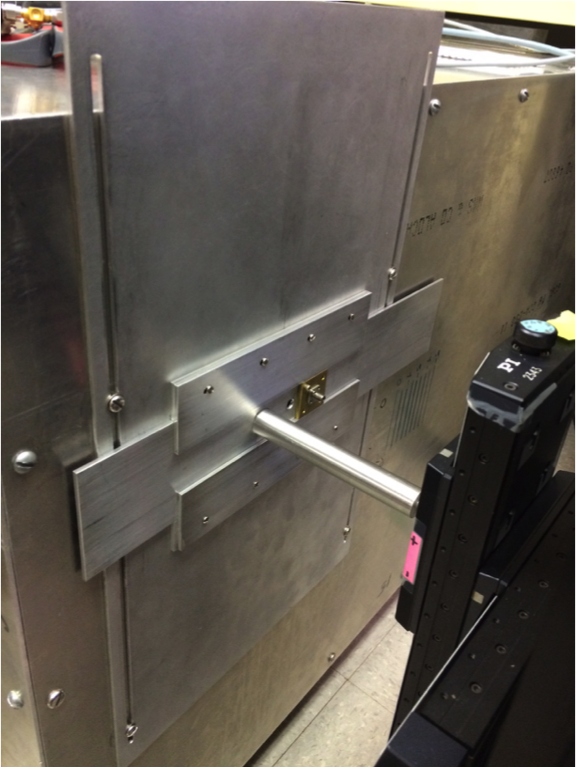
\includegraphics[width=0.75\textwidth]{moving/mikro-move-1}
    \caption[MikroMove Translation Stage]{The PI MikroMove translation stage (black, right) attached to a sliding window on the Gigabox (left) via a metal arm. The antenna is attached to the sliding window just to the right of the arm. The MikroMove translates the arm up (+) and down (-), which moves the sliding window and ultimately the antenna along the same range of motion. This particular model had a maximum range of motion of 70~mm along a single axis.}
    \label{fig:mikro-move}
\end{figure}


\subsubsection{Results}
\label{sec:spatial-results}

We repeated the experiment described above for carrier frequencies in the range 4-9~GHz and display these results in~\ref{fig:spatial-freq-profile}. Differences in amplitude between the curves are due to differences in $S_{1,2}$ parameters between frequencies for our particular antennas.

\begin{figure}
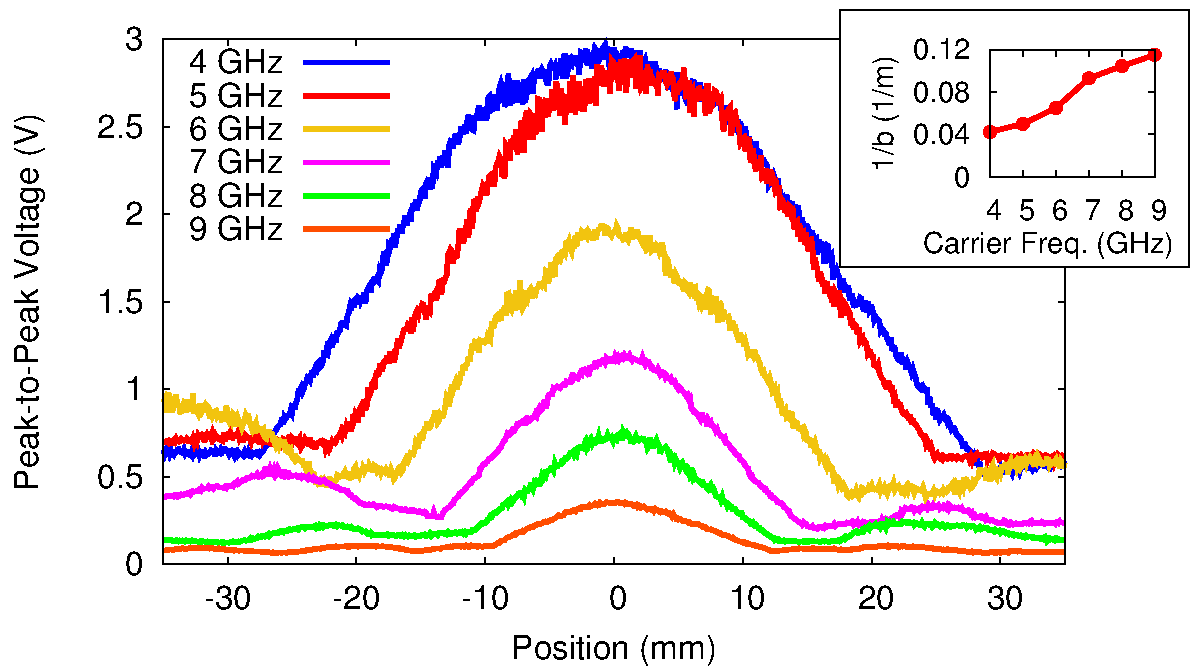
\includegraphics[width=\columnwidth]{spatial/freq_profile.pdf}
\caption[Spatial profile of reconstruction at various frequencies]{Spatial profile of \ptp{} voltage of reconstructions investigated at carrier frequencies ranging from 4 to 9 GHz in 1 GHz
steps.  The inset shows the inverse of the fit $b$ values versus carrier frequency, showing the expected linear relationship.}
\label{fig:spatial-freq-profile}

\vspace*{\floatsep}% http://tex.stackexchange.com/q/26521/5764

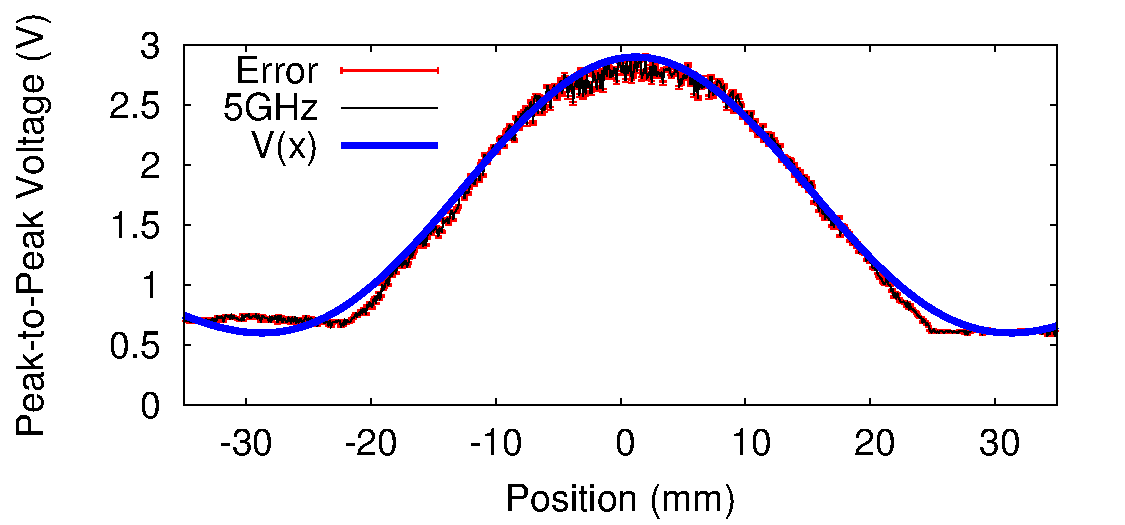
\includegraphics[width=\columnwidth]{spatial/fit.pdf}
\caption[Fit of spatial profile]{Measured \ptp{} voltage of reconstructions received in the
vicinity of a time-reversed wave collapse location with a 5 GHz carrier
frequency, and fit to the \texttt{sinc(x)} function. The parameters here are $a = 2.18 \pm 0.046397869$, $b = 26.72 \pm 0.134629783$, $c = -73.58 \pm 0.116338652$, and $d = 0.43 \pm 0.012711137$. The fit parameters for the remaining 4-9~GHz frequency profiles from Figure~\ref{fig:spatial-freq-profile} are given in Appendix~\ref{app:spatial-fit-params}.}
\label{fig:spatial-error-fit}
\end{figure}

Based on observations from the results in Figure~\ref{fig:spatial-freq-profile}, we expect the reconstruction \ptp{} voltage profile to take the form of a $sinc(x)$ function about the target location~\cite{lerosey-focusing}. Thus, we propose the following equation to predict $V(x)$, the maximum \ptp{} voltage from a given reconstruction, as a function of $x$, the distance between the reconstruction focal point and the receiver:

\begin{equation}
\label{eq:vx}
V(x) = a\cdot sinc\left(\frac{x+c}{b}\right) + d
\end{equation}

where $a$ is the maximum \ptp{} reconstruction amplitude, $b$ is the half-wavelength, $c$ is the location of the antenna along the x-axis, and $d$ is the noise level offset voltage. Since $b$ is proportional to the wavelength (and inversely proportional to frequency), as the carrier frequency is increased,  $\frac{1}{b}$ also increases, causing the ``bubble'' of the sinc function in Figure~\ref{fig:spatial-freq-profile} to get smaller. This relationship is shown explicitly in the inset of Figure~\ref{fig:spatial-freq-profile}. Figure~\ref{fig:spatial-error-fit} shows Equation~\ref{eq:vx} fit to the 5 GHz curve from Figure~\ref{fig:spatial-freq-profile}, including error bars. The fit qualitatively looks good around the main lobe, but quantitatively has a high reduced $\chi^2$ value, primarily due to the rather large background noise level that has hidden the side lobes. Fitting to just the main lobe produces a much better goodness of fit metric. The error bars are primarily systematic, introduced by the oscilloscope internal voltage multiplier used in scaling.

The results presented in Figure~\ref{fig:spatial-freq-profile} allow us to draw several conclusions. In this frequency range, the reconstructions can be categorized as broad, spanning several centimeters in width. This is significant because it indicates that we can move the receiver slightly away from the target location and still collect energy from the reconstruction. This allows us to implement a system targeting a moving receiver.

\subsection{Reconstructing on a Moving Target}
\label{sec:recon-moving}

\subsubsection{Methodology}
For this experiment, the receiving antenna was moved at a constant speed of 0.2~$\frac{mm}{s}$ across the entire 70~mm range provided by the translation stage. To counteract the degradation of reconstruction strength as the antenna moved, we periodically repeated the interrogation step, effectively re-centering the reconstruction on the antenna. Since the test equipment does not allow broadcast of one sona while collecting another, it was not possible to transmit power during the collection time, leading to a finite ``dead time,'' denoted $t_d$ in Figure~\ref{fig:moving-recon}. During the broadcast period, the time-reversed sona was continually broadcast into the cavity (once every 15~$\mu$s) and the peak-to peak voltage across the receiver was measured once every 2.05~seconds, meaning that the reconstructions are highly undersampled in this plot. After every 15 samples were collected, the process was repeated. We refer to this full process of collecting a new sona and then broadcasting it for a given period time as a full ``cycle'' of length $t_c$. The results in Figure~\ref{fig:moving-recon}  below were obtained using a carrier frequency of 5 GHz, $t_d$ of 7 seconds, and $t_c$ of 39.8 seconds. Based on the results from Section~\ref{sec:spatial-results}, the \ptp{} reconstruction voltage measured by the receiver is expected to decay according to the $sinc(x)$ function as the receiver moves away from the reconstruction focal point. This $sinc(x)$ function will be centered on the position where the sona was last collected, making the reconstruction focus continually lag behind the antenna. Consequently, the maximum reconstruction strength is limited by the time needed to collect, time reverse and re-broadcast an updated sona. The following equation is proposed as a model for the \ptp{} voltage of the reconstruction on a moving target as a function of time, assuming a constant velocity $\bar{v}$:

\begin{equation}\label{eq:vt}
%\begin{displaymath}
  V(t) = \left\{
        \begin{array}{ll}
                0 & : t\pmod{t_c} \le t_d \\
                a\cdot |sinc(\frac{\bar{v}t}{b})|+d & : t\pmod{t_c} > t_d
        \end{array}\,.
  \right.
%\end{displaymath}
\end{equation}

\subsubsection{Results}
\label{moving-results}

The results of this experiment are very promising. We hypothesized that the reconstruction \ptp{} voltage would reset back to a maximal value when a new sona was used to refocus the reconstruction, and follow the voltage profile as the receiver moved away from the new target location. This was almost exactly confirmed by the experimental results. This is encouraging for the application of TR to a practical WPT scheme because it proves the applicability to a moving receiver system.

\begin{figure}[t]
\centering
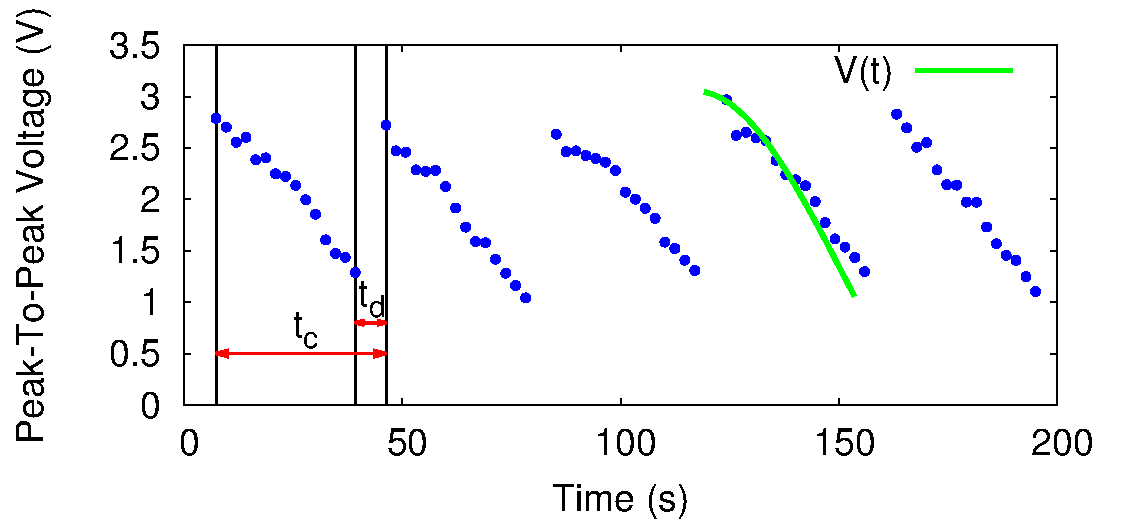
\includegraphics[width=0.85\textwidth]{moving/moving_recon}
    \caption[\Ptp{} voltage of moving reconstructions]{Reconstruction \ptp{} voltage vs. time as the target moves along one wall of the enclosure. A new sona signal is acquired every $t_c = 39.8s$, leading to a dead time of duration $t_d = 7s$. The target is moving at a speed of 0.5~$\frac{mm}{s}$ and the carrier frequency is 5~GHz. The green line is Eq.~\ref{eq:vt}.}
    \label{fig:moving-recon}
\end{figure}

It is worth noting that the speed of the receiver is relatively slow at 0.2~$\frac{mm}{s}$. This experiment is intended to be a proof of concept, with generalized equipment that carries significant overhead. The GPIB connections between the signal generators, oscilloscope, and workstation contributed to the long delay between system operations, in addition to the slow processing speed of the equipment itself. We expect that with a dedicated time reversal system, the TR process of reacquiring a new target location could be performed in milliseconds and describe the ramifications for doing so in Section~\ref{sec:future-timing}. This would greatly increase the maximum receiver speed that could be accommodated as the reconstruction could be refocused more often, and thus the average \ptp{} voltage could be raised closer to that maximal value. We conclude that, with further research and engineering work, a TR WPT scheme could feasibly power a moving receiver in realistic scenarios.

\section{Timing and Computational Complexity}
\label{sec:future-timing}

In Section~\ref{sec:moving}, we showed that the ability of a time reversal system
to transmit energy to a moving target is dependent on the spatial profile and
transmission dead time, $t_{d}$.
%
In this work, our equipment limited us to a $t_d$ of 7~seconds, which would be too slow
to handle most typical movement, such as walking across a room.
%
The primary bottlenecks here were the communication between the oscilloscope
and computer, and the fast Fourier transform (FFT) operations performed in MATLAB
on the computer.
%
A practical system could overcome these limitations by combining the two components
into a single device, which would remove the communication overhead, and optimizing for
the FFT computation in hardware.
%
Once a sona has been recorded (shown in Figure~\ref{fig:sona} to be on the order of 10~$\mu$s),
the theoretical lower bound on processing time would be limited only by the amount of
time required to compute an FFT.

\begin{figure}[t]
\centering
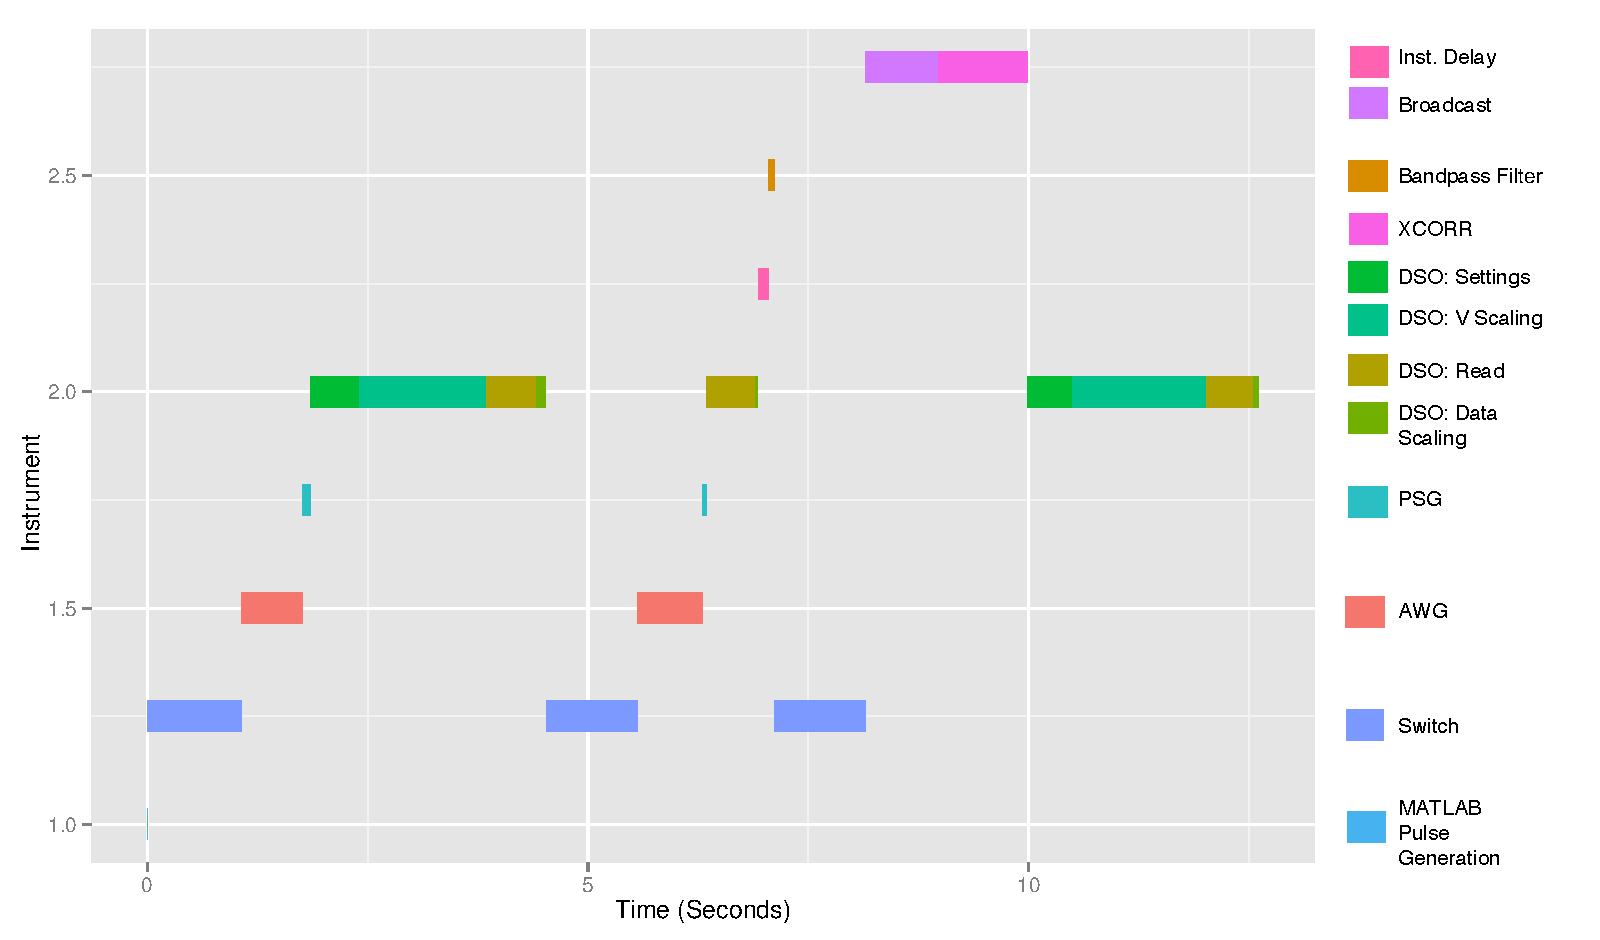
\includegraphics[width=\columnwidth]{future/timing}
\caption[Timing Analysis of Experimental Setup]{}
\label{fig:timing}
\end{figure}



\chapter{Nonlinear Time Reversal}
\label{ch:nltr}

\section{Purpose and Conceptual Overview of Nonlinear Time Reversal}
\label{sec:nltr-purpose}

The preceeding chapters have been concerned with linear time reversal, or LTR, and have focused primarily on investigating properties of reconstructions. Now, we move into our nonlinear/NLTR investigations, which focus on proof of concept of targeting capabilities. As a reminder, NLTR makes use of harmonic reflections from the target to isolate it via frequency domain inspection after the sona is collected, a process similar to how we would envision a TR based WPT system to work. 

Conceptually, our general process is this: we broadcast a Gaussian pulse from one port serving as both the transmitter and the receiver. Elsewhere in the Gigabox is a nonlinear element serving as a target. Any reflections from this element will contain harmonics: frequency components at multiples of the original frequency. These harmonics are embedded along with all the other echos in sona collected back at the transceiving port. However, before time reversing the sona, we transform it into the frequency domain and filter out all the components not within some band of the harmonic frequencies. In this way, we isolate only those wave paths that had contact with the nonlinear target. That filtered sona is time reversed and rebroadcast from the transceiving port, which will cause a slightly distorted version of the original Gaussian pulse to reconstruct at the target. This process is illustrated in Figure~\ref{fig:nonlinear-diagram}.

\begin{figure}[h!]
\centering
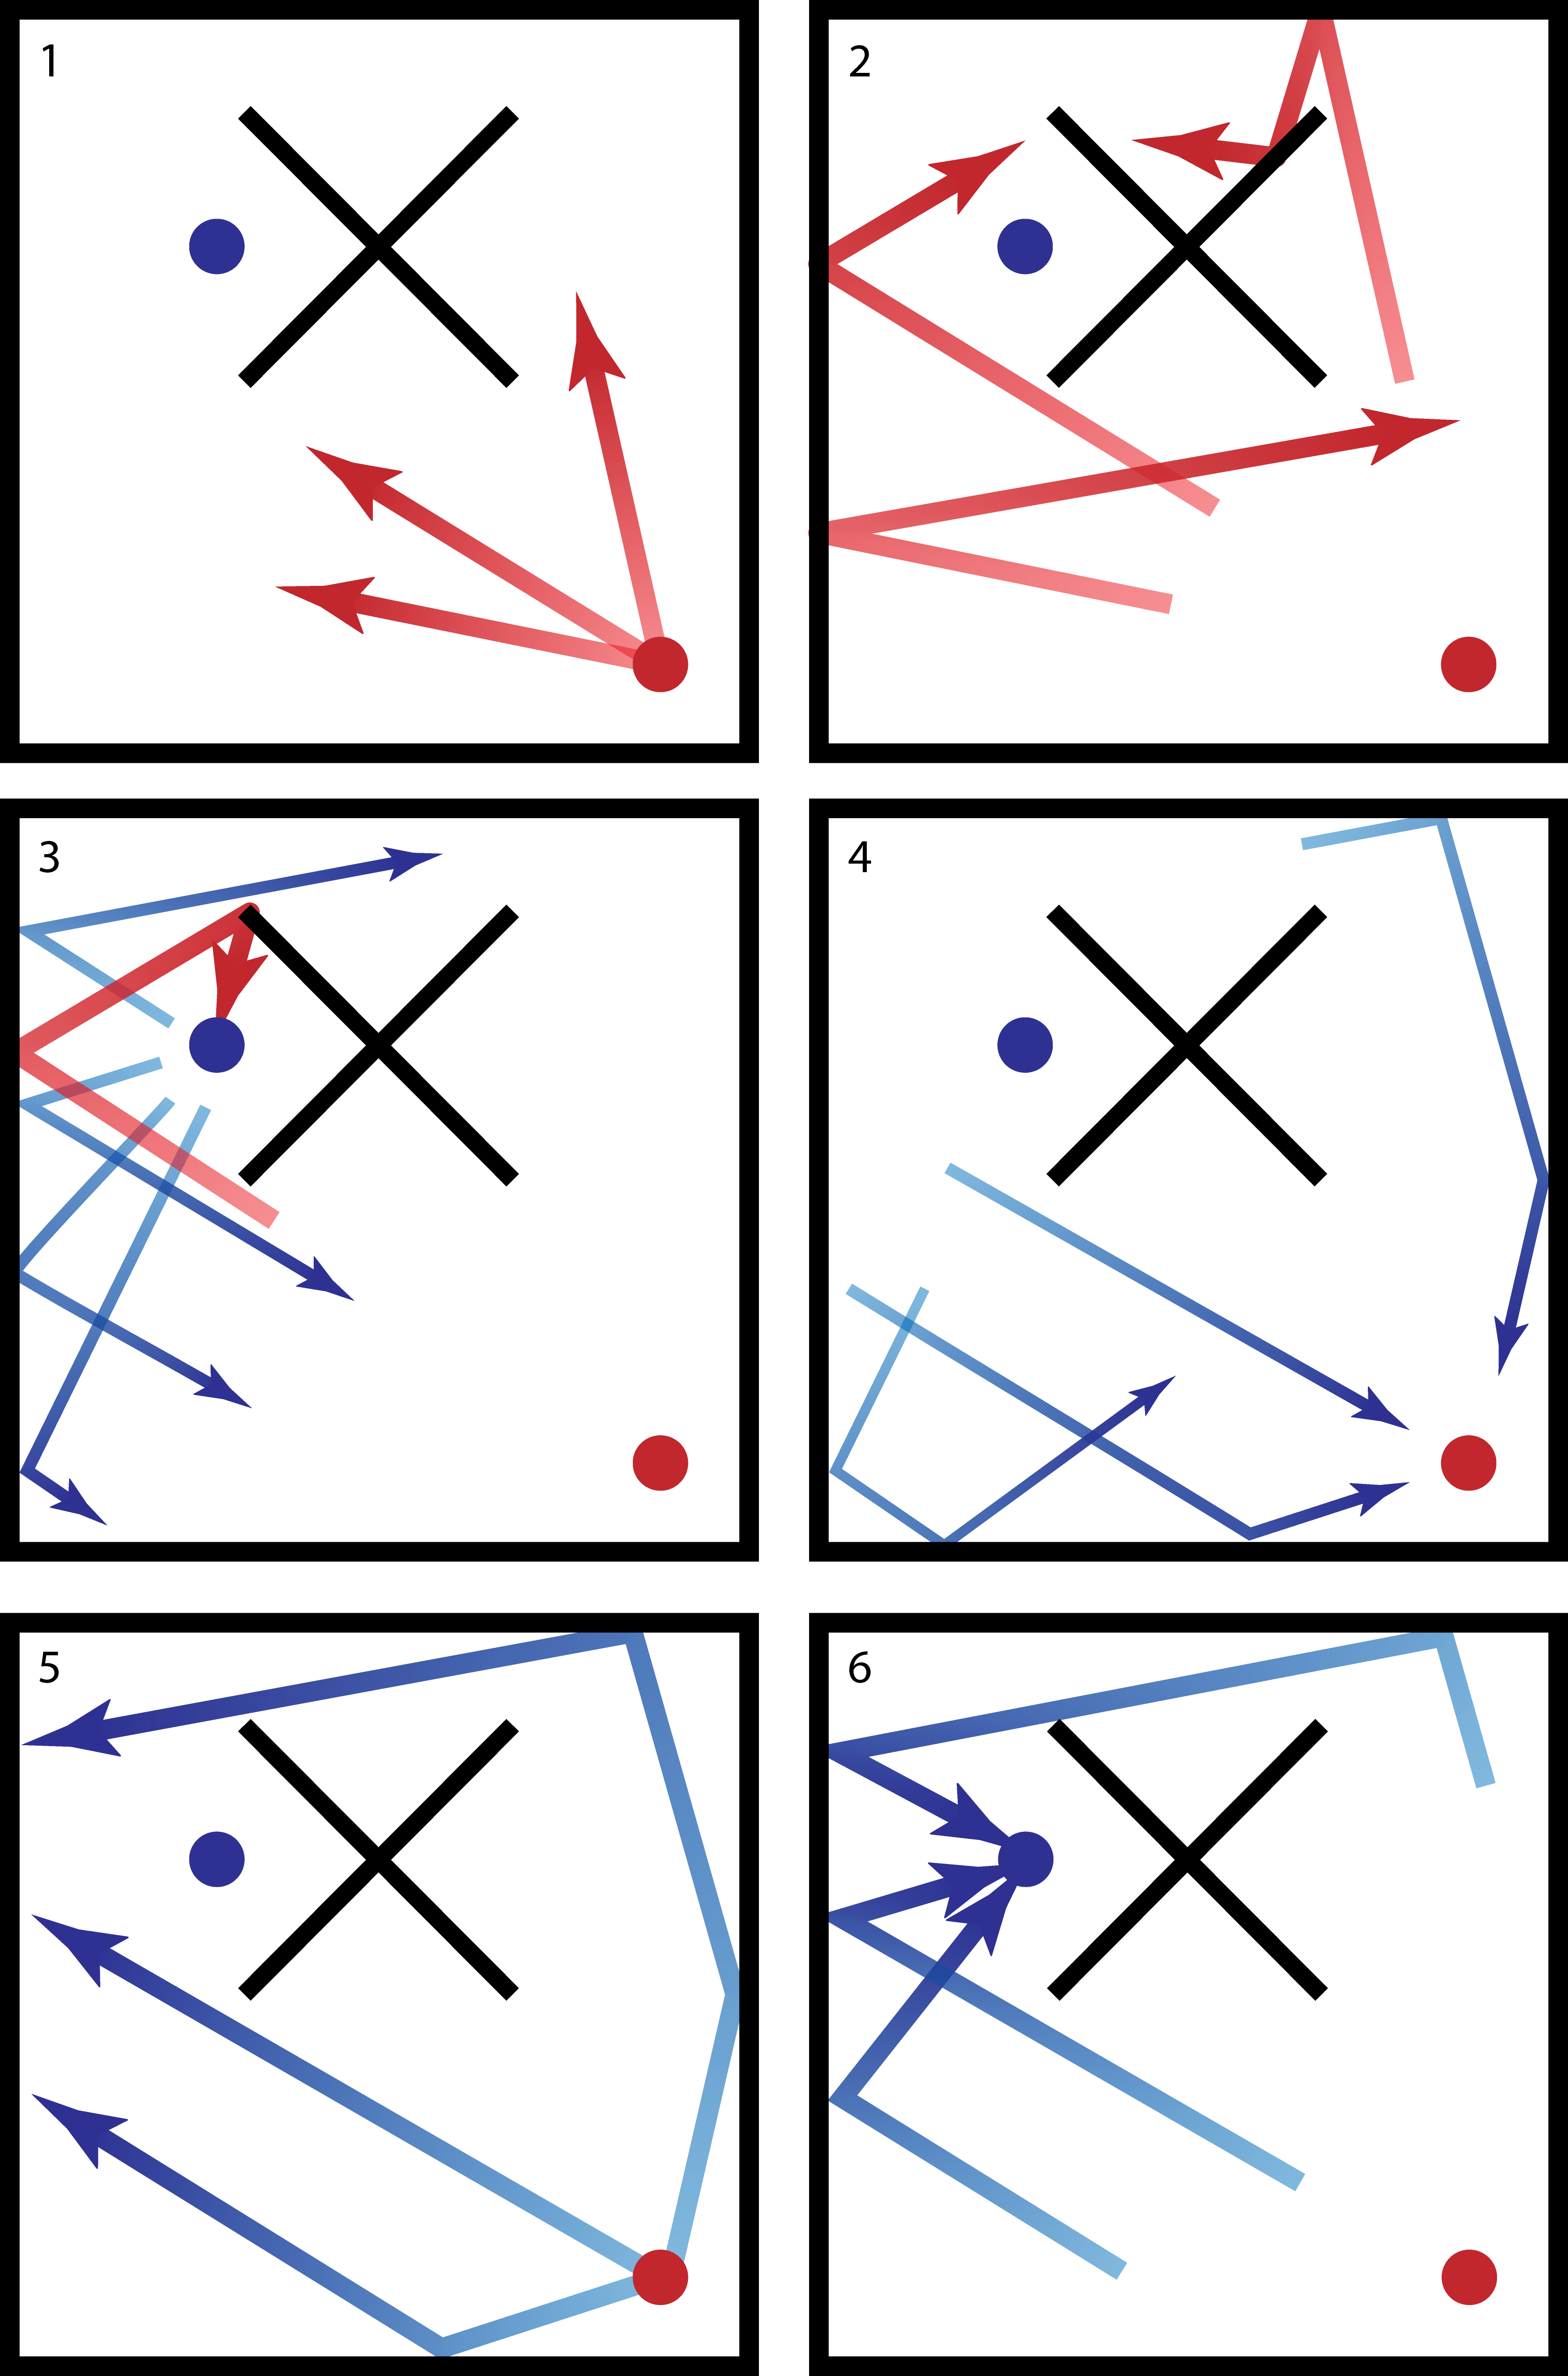
\includegraphics[width=0.85\textwidth]{nonlinear/diagram}
    \caption[Conceptual overview of nonlinear time reversal]{Reading order from top left: (1) The TRM broadcasts a signal into the cavity at one frequency, which (2) reverberates within the cavity. Eventually, (3) the signal reaches the nonlinear element somewhere within the chamber. Reflected waves that encounter this element will have a characteristic frequency signature containing harmonics of the original signal. (4) Some of these harmonic reflections will find their way back to the TRM. the TRM filters the sona to extract only those reflections, then time reverses and (5) re-emits them. (6) The time reversed waves collapse back on the nonlinear target.}
    \label{fig:nonlinear-diagram}
\end{figure}

We explored several different applications of NLTR with an eye towards adapting the technique for WPT, both experimentally and in simulation. The experimental portions met with limited success due to the diffculty of passively producing harmonics of significant magnitude. However, we believe the the applications of NLTR as a WPT method remains feasible. Discussion of the difficulties that set back our work will be presented in the "Future Works" section in the Conclusion. Successful results, including those of numerical simulations, are explored at length in the following NLTR sections. 

\section{Experimental Difficulties}
\label{sec:nltr-expr-diff}

\subsection{Ferromagnetic Nanorods as a Nonlinear Beacon}

In order to generate a harmonic response, the nonlinear object must possess inherent nonlinearity in its material properties. Since TR uses electromagnetic waves, we are interested in possible nonlinear electric or magnetic properties. In this section, we discuss a potential magnetic nonlinear object in the form of ferromagnetic nanorods. These nanorods have a nonlinear magnetization curve. This means that the B-field generated from an interrogation signal should have a harmonic response that we may use for NLTR.

While the usage of diodes as nonlinear objects has been well-documented, the usage of ferromagnetic nanorods as nonlinear objects has not. As a result, we had to perform preliminary experiments on the ferromagnetic nanorods in order to verify that the nonlinear response was strong enough to successfully complete the NLTR process.

This preliminary experiment consisted of sending a pulse signal into an antenna with the ferromagnetic nanorods attached to them and recording the response signal. By transforming the response signal to the frequency domain, we were able to easily identify whether or not a $2f$ harmonic was generated.

 \begin{figure}
     \centering
     \begin{subfigure}{0.45\textwidth}
         \centering
         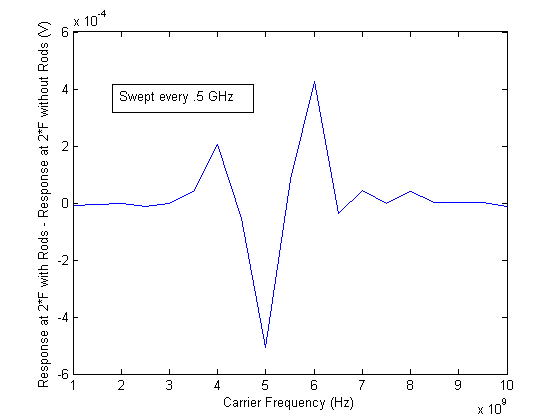
\includegraphics[width=1.0\linewidth]{nanorod/exp-1}
         \caption[]{}
         \label{fig:nanorod-exp-1}
     \end{subfigure}
         \begin{subfigure}{0.45\textwidth}
         \centering
         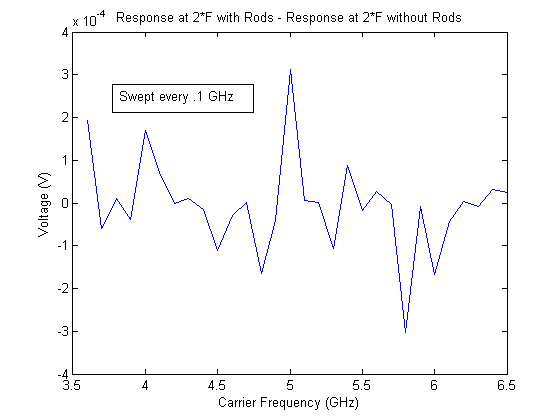
\includegraphics[width=1.0\linewidth]{nanorod/exp-2}
         \caption[]{}
         \label{fig:nanorod-exp-2}
     \end{subfigure}
         \begin{subfigure}{0.45\textwidth}
         \centering
         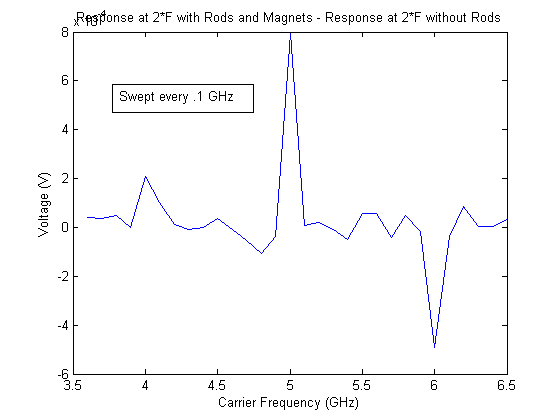
\includegraphics[width=1.0\linewidth]{nanorod/exp-3}
         \caption[]{}
         \label{fig:nanorod-exp-3}
     \end{subfigure}
         \begin{subfigure}{0.45\textwidth}
         \centering
         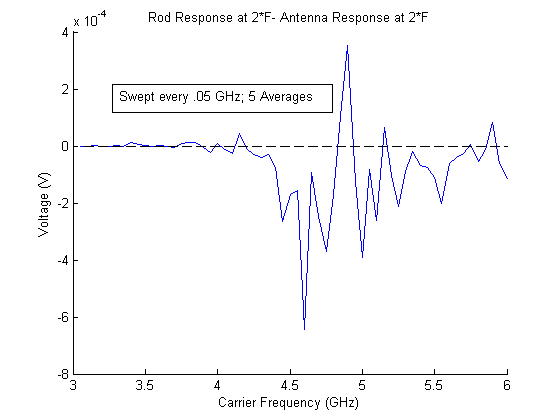
\includegraphics[width=1.0\linewidth]{nanorod/exp-4}
         \caption[]{}
         \label{fig:nanorod-exp-4}
     \end{subfigure}
     \caption[Ferromagnetic nanorod experimental results]{Experimental results. (a) - (d) show various ferromagnetic nanorod configurations. No configuration leads to a significant $2f$ response, as illustrated through the random and small amplitude response signals}
     \label{fig:nanorod-results}
 \end{figure}

  Figure~\ref{fig:nanorod-results}(a)-(d) show the $2f$ response under a variety of conditions. Although there seem to be peaks in (a) - (d), the peaks are somewhat randomly distributed and are small in magnitude. Due to these two aspects of our preliminary testing, we determined that using ferromagnetic nanorods as a potential magnetic nonlinear object was infeasible for performing NLTR.

\subsection{Diodes as an Electric Nonlinear Beacon}

While utilizing a nonlinear magnetic response was not feasible, utilizing a nonlinear electric response has been well-documented through the use of a diode. This represents a nonlinear object, as the current response to an applied voltage for a diode changes significantly after a certain applied voltage value, as seen in Frazier et al. have previously used diodes in NLTR experiments to much success.

We performed another preliminary test to verify the nonlinear response of a diode after being interrogated by a Gaussian pulse. Given the history of diodes in NLTR, we believed that we would see a large $2f$ response. While performing these preliminary tests we were unable to produce any measurable harmonic from a diode while it was present in the \giga{}. In order to circumvent this problem, we used extremely large amplifiers as done by Hong et al. in their NLTR experiments. We were still unable to generate a significant harmonic response.

As a last effort we used various frequency multipliers to generate a nonlinear signal. We did this to verify that the equipment used in our setup was functioning properly. We were able to extract a nonlinear sona from the frequency multiplier; however, this is infeasible in a WPT technology as frequency multipliers are large in size. This confirmed that our equipment was working properly but that we were unable to generate a large response. Due to not being able to generate a nonlinear sona experimentally, we conducted all of our NLTR experiments using numerical simulation.

\section{Purpose}
\label{sec:numerical-purpose}

Here, we focus entirely on numerical simulations of NLTR as they apply to WPT. Our focus was threefold: (1) to conduct simultaneous NLTR collapses onto two nonlinear objects, (2) to observe the selective collapse of NLTR onto two distinct nonlinear objects, and (3) to characterize the transmission efficiency of the process. From these three focuses, we demonstrated that the NLTR process may be generalized to an arbitrary number of nonlinear objects in an enclosure and that these reconstructions may be selectively rectified at the nonlinear objects. We provide a scheme to characterize the efficiency of our process but were unable to develop a conclusive theory for tuning the efficiency. Our results provide a baseline for developing an experimental algorithm for targeting objects in an enclosure for WPT applications, either selective or non-selectively.  We will first detail the general scheme used for performing NLTR and follow with the setup, experimental results, and discussion for each of our three focus topics.

The process of developing a new technology required benchmarking each step diligently. Any successful WPT technology must have effective transmission efficiency, implying minimal loss in each step of the system. Given the broad frequency signals used in experimentation, a significant drawback to any TR experiment is the inherent wave reflection at interfaces between equipment, various mediums, or circuitry~\cite{smith_waves_2010,griffiths_david_introduction_1999}. While wave reflection losses can be theoretically be measured via S Parameters (explained later) of an experiment, these sources of loss are not practically measurable due to the fact that measuring the losses would create addition interfaces in the system, introducing additional sources of wave reflection~\cite{smith_waves_2010}. To calculate the true ceiling on effective transfer efficiency, it is necessary to numerically simulate the process, as a simulation can calculate the various losses without interfering with the system itself.

In addition to using simulations to study the sources of loss in our system, it also provided us with a simple nonlinear element: a model diode. As explained in previous chapters, the nonlinear response in our \giga experiments was found to be difficult to excite due to power limitations, noise, or equipment sensitivity. The difficulties that we encountered in our physical experimentation were circumvented by numerically simulating the NLTR process. By being able to monitor the voltage and current response of the diode at all times in the simulation, we were able to troubleshoot problems that occurred in the numerical NLTR process that would have otherwise have been impossible to determine in experimentation.

\section{Methodology}
\label{sec:numerical-meth}

\subsection{Equipment}
In order to perform these tests that were not possible in the \giga, we used the program Computer Simulation Technology: Microwave Studio (CST for short) to perform electromagnetic wave simulations. CST is an industry standard modeling program that uses the Finite Integration Technique (FIT) to numerically solve Maxwell's equations~\cite{computersimulationtechnology}. This technique is a generalized version of the well-known Finite Difference Time Domain (FDTD) method but can resolve complex geometries and boundary conditions in a simpler manner. We will not discuss these techniques at length, as they are well-understood in the literature~\cite{schneider2010understanding,weiland2001discrete}.
Our team had two computers with a total of two shared CST licenses to perform simulations. The processing power, RAM, and GPU availability are shown below in Table~\ref{tab:numerical-cpu-specs}. CPU A was used for either single simulations or computationally small simulations. A single simulation refers to a simulation where we did not sweep a parameter.  CPU B was used for large simulations or parameter sweep simulations, requiring either large amounts of memory or large amounts of time, respectively. In general, we used CPU A to perform simultaneous and selective NLTR while we used CPU B to calculate transfer efficiency and characterize nonlinear response characteristics.

\def\arraystretch{2}
\begin{table}[h]
\centering
\begin{tabular}{|l|l|l|}
\hline
 & \textbf{CPU A} & \textbf{CPU B} \\ \hline
Processor & \rule{0pt}{2.5em}\shortstack{Intel Xeon CPU \\ X5670 @ 2.93~GHz} & \rule{0pt}{2.5em}\shortstack{Intel Xeon CPU \\ E5-2680 @ 2.50~GHz} \\ \hline
Number of Processors & 2 & 2 \\ \hline
RAM & 44 GB & 128 GB \\ \hline
GPU Available & No & Yes \\ \hline
\end{tabular}
\caption[Computer specifications]{Technical specifications of the computers used for conducting all simulations and modeling.}
\label{tab:numerical-cpu-specs}
\end{table}

\subsection{Time-Reversal and Nonlinear Sona Extraction}
To start any simulation, we first generated a Gaussian pulse signal in \matlab. For this interrogation signal, we chose the amplitude, center frequency, and bandwidth frequency for our experiment. An example input signal is shown inset in Figure~\ref{fig:numerical-input-wave}. The simulation was run using this pulse signal, noting one of the ports as an injection port (e.g. Port A) and one as the recording port (e.g. Port B).


\begin{figure}[t]
\centering
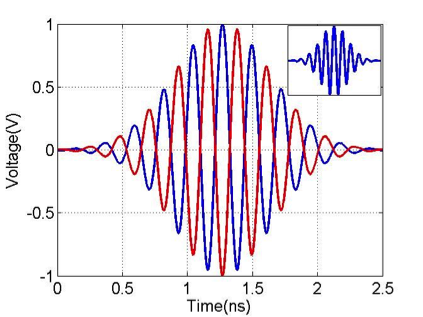
\includegraphics[width=0.85\textwidth]{numerical/input-wave}
\caption[Example of inverted and non-inverted interrogation signals]{This shows our input waveform with a 4.4~GHz center frequency and 1.0~GHz bandwidth. The blue signal is the non-inverted input and the red signal is the inverted input. A singular, non-inverted waveform is shown in the inset.}
\label{fig:numerical-input-wave}
\end{figure}

In general, we had two methods to extract the nonlinear sona from our recorded signal: (1) applying a Fourier transform and band-pass filtering the raw signal and (2) pulse inversion. As previously discussed, many of the \giga experiments were performed by recording a sona, applying a Fast Fourier Transform (FFT), and finally using a band-pass filter on the recorded signals to extract the harmonic signal at the correct frequency. In our numerical simulations; however, the sonas were only recorded for \numrange{30}{35}~ns and the discretized nature of the data on this time scale led to distortion of the sona signals.
The team also explored using pulse inversion, another method of sona extraction that has been well documented in the literature~\cite{simpson_pulse_1999,hong_nonlinear_2014}. Hong et al. have used this method for numerous time-reversal experiments, citing its computational simplicity as a benefit for using it in physical experiments~\cite{hong_nonlinear_2014}. The process involves summing two sonas with inverted inputs.  When the sonas are summed, linear signals are cancelled out, and nonlinear signals remain. Adding the sonas is significantly faster than applying a transformation to an entire sona signal, saving time. While this process proved to be very difficult to implement for our \giga experiments, it was quite efficient at producing the nonlinear sona in CST.
Due to the simplicity of pulse inversion, we used this method for extracting all nonlinear sonas. In this method, we ran the same simulation once with our original input signal and then we ran it a second time with an inverted version of our original signal. Inversion simply means that the entire original signal was multiplied by $-1$. Assuming a linear system, the sum of the original and inverted signals sums to $0$; however, a nonlinear system sum is non-zero. Because the diode is the only nonlinear portion of the system, summing the original and inverted signals yields only the signal from the diode, which is the desired nonlinear sona. Figure~\ref{fig:numerical-sonas}(a) and (b) illustrate two sona signals, where the blue signal is the non-inverted sona and the red signal is the inverted sona. Figure~\ref{fig:numerical-sonas}(b) contains a nonlinear element while~\ref{fig:numerical-sonas}(a) does not. The corresponding (c) and (d) show the result of summing the two signals. It is clear that total annihilation of the sona signal occurs when no nonlinear element is present, as in~\ref{fig:numerical-sonas}(c), while a clear signal is present in~\ref{fig:numerical-sonas}(d).


\begin{figure}[t]
\centering
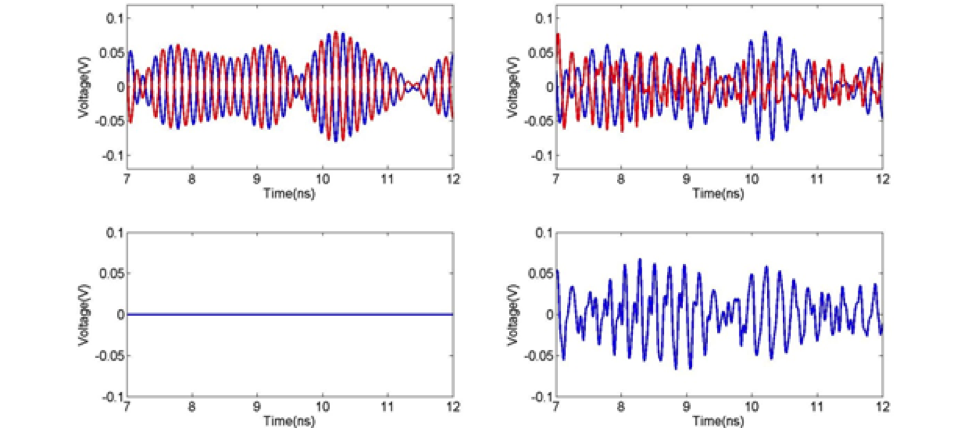
\includegraphics[width=0.85\textwidth]{numerical/sonas}
\caption[Demonstration of pulse inversion]{(a) shows a portion of the non-inverted (blue) and inverted (red) recorded response signal. (b) shows the same two response signals when a diode is present in the simulation. (c) the sum of the two signals in (a), resulting in signal annihilation. (d) the sum of the two signals in (b), which produce a non-zero signal.}
\label{fig:numerical-sonas}
\end{figure}
This method to extract the nonlinear sona was chosen over taking the FFT and filtering the recorded signal as sample rate for the simulation data was not high enough to ensure the results would not be distorted. This discretization of data caused the resulting time-reversed sonas to produce incorrect results using the FFT and filter method, while the time-reversed sonas produced correct results with the pulse inversion method.
\subsection{Defining and Controlling the Nonlinear Element}
In the simulations themselves, we used a model diode as our nonlinear object, as it has a nonlinear I-V curve. The diode location for each simulation was chosen semi-arbitrarily with the only restriction to not be within \numrange{1}{2} wavelengths of either port, as this may have created near-field effects that influenced the results. In CST, the diode component is modeled as the following circuit (Figure~\ref{fig:numerical-cst-diode}) and mathematical relationship (Equation~\ref{eq:numerical-vd-gt-0} and~\ref{eq:numerical-vd-lt-0}). From these, the user may change the parasitic capacitance ($C$), the series resistance ($R$), the reverse conductance ($G_{s}$), and the functional temperature ($T$).

For $V_d > 0$:

\begin{equation}
I_d = I_0\left( e^{\frac{eV_{d}}{kT}-1}\right) = I_0\left( e^{\frac{V_{d}}{V_{k}}a - 1}\right)
\label{eq:numerical-vd-gt-0}
\end{equation}

For $V_d < 0$:

\begin{equation}
I_{d} = G_{s}V_{d}
\label{eq:numerical-vd-lt-0}
\end{equation}


To obtain idealized results, we set $C$ and $G_s$ to $0$, as these values reduced the magnitude of the nonlinear response. We used the default $R = 50 \Omega$, as very large $R$ reduced the overall signal greatly and a very small $R$ did not produce any harmonics. This left only $T$ to tune the I-V curve of the diode. In real life, different diodes have different I-V curves based on material. In order to simulate these differences mathematically, we changed the temperature of the diode in the simulation, as shown in Figure~\ref{fig:numerical-iv-curves}.

In reality, this changed the knee voltage ($V_{k}$) for the diode. We chose $V_{k}$ to be the applied voltage needed to achieve a current of $0.2 I_{0}$. The parameter $a$ is used to define this $0.2 I_{0}$ cutoff. As discussed later in this chapter, we will show how the nonlinear response of a diode is dependent on both the input pulse amplitude and the knee voltage. This nonlinear response was maximized to allow for selective targeting between two diodes simultaneously.
\section{Results}
\label{sec:numerical-results}

\begin{figure}[]
\centering
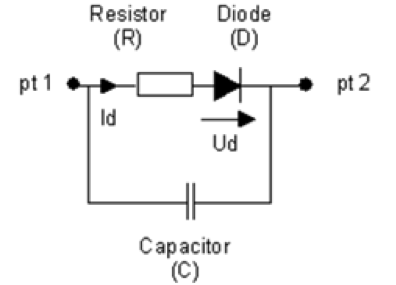
\includegraphics[width=0.7\textwidth]{numerical/cst-diode}
\caption[CST diode circuit model]{CST diode circuit model}
\label{fig:numerical-cst-diode}

\vspace*{\floatsep}% http://tex.stackexchange.com/q/26521/5764

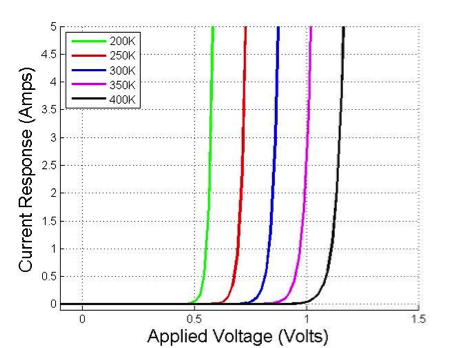
\includegraphics[width=0.7\textwidth]{numerical/iv-curves}
\caption[I-V curves of diodes with different voltage knees]{Different I-V curves that can be modeled in CST. It should be noted that the ``Temperature'' of the diode only changes its mathematical definition of the I-V curve}
\label{fig:numerical-iv-curves}
\end{figure}

\subsection{Simultaneous Nonlinear Time Reversal}

The first focus of our numerical simulations was to illustrate the collapse of a nonlinear time-reversed sona on multiple targets simultaneously. To be an effective WPT system, our technology would need to be able to charge more than one device at a time. Based on literature illustrating NLTR collapsing on a single nonlinear object, we hypothesized that a nonlinear sona would collapse on an arbitrary number of nonlinear objects if the nonlinear objects were present in the time-forward step of NLTR~\cite{nltr-classical-waves,nltr-wave-chaotic}. We assumed that the reconstruction on each nonlinear object would sum linearly and independently such that no reconstruction would interfere with another, as shown in Equation~\ref{eq:numerical-r-tot}, where $R_{i}$ is the reconstruction on a single nonlinear object and $x_{i}$ is a weighting of the amount of power that the single nonlinear object contributes to the overall power of all reconstructions. Based on this, we expected the reconstruction waveforms of the independent single-diode simulations to match a single, multi-diode simulation.

\begin{equation}
R_{tot} = \sum_{i} R_{i}x_{i}
\label{eq:numerical-r-tot}
\end{equation}

This feature was realized by creating a geometry with two diodes present along with two ports to record and emit signals, shown below. We created a quasi-two-dimensional (2D) irregular cavity in CST. This cavity was a 15cm x 15cm x 0.76cm square box modified with various circular and elliptical segments removed from the walls as shown in Figure~\ref{fig:numerical-cst-box}.  The 0.76cm height was chosen to maintain a 2D simulation. Equation~ref{eq:numerical-cutoff-freq} was used to calculate the cutoff frequency for the fundamental mode of a parallel plate cavity, below which only 1 frequency will propagate, reducing the time needed to simulate~\cite{griffiths_david_introduction_1999}.

\begin{equation}
f_c = \frac{c}{2h}
\label{eq:numerical-cutoff-freq}
\end{equation}

Using a cavity of height 0.76 cm resulted in a cutoff frequency of 20~GHz, well above our typical test frequencies of \numrange{4}{5}~GHz fundamental and \numrange{8}{10}~GHz harmonic. We chose this cutoff frequency in the event we needed to use a higher fundamental frequency to create better spatial resolution of our reconstruction. The area dimensions for the Cut Box Model were chosen to minimize computational time while still maintaining a reasonable mode density, as shown in Figure~\ref{fig:numerical-cst-box}(a). This mode density is required to allow the ray chaotic environment to have high sensitivity to initial and boundary conditions; a low mode density will prevent NLTR from having high spatial resolution.

\begin{figure}[t]
\centering
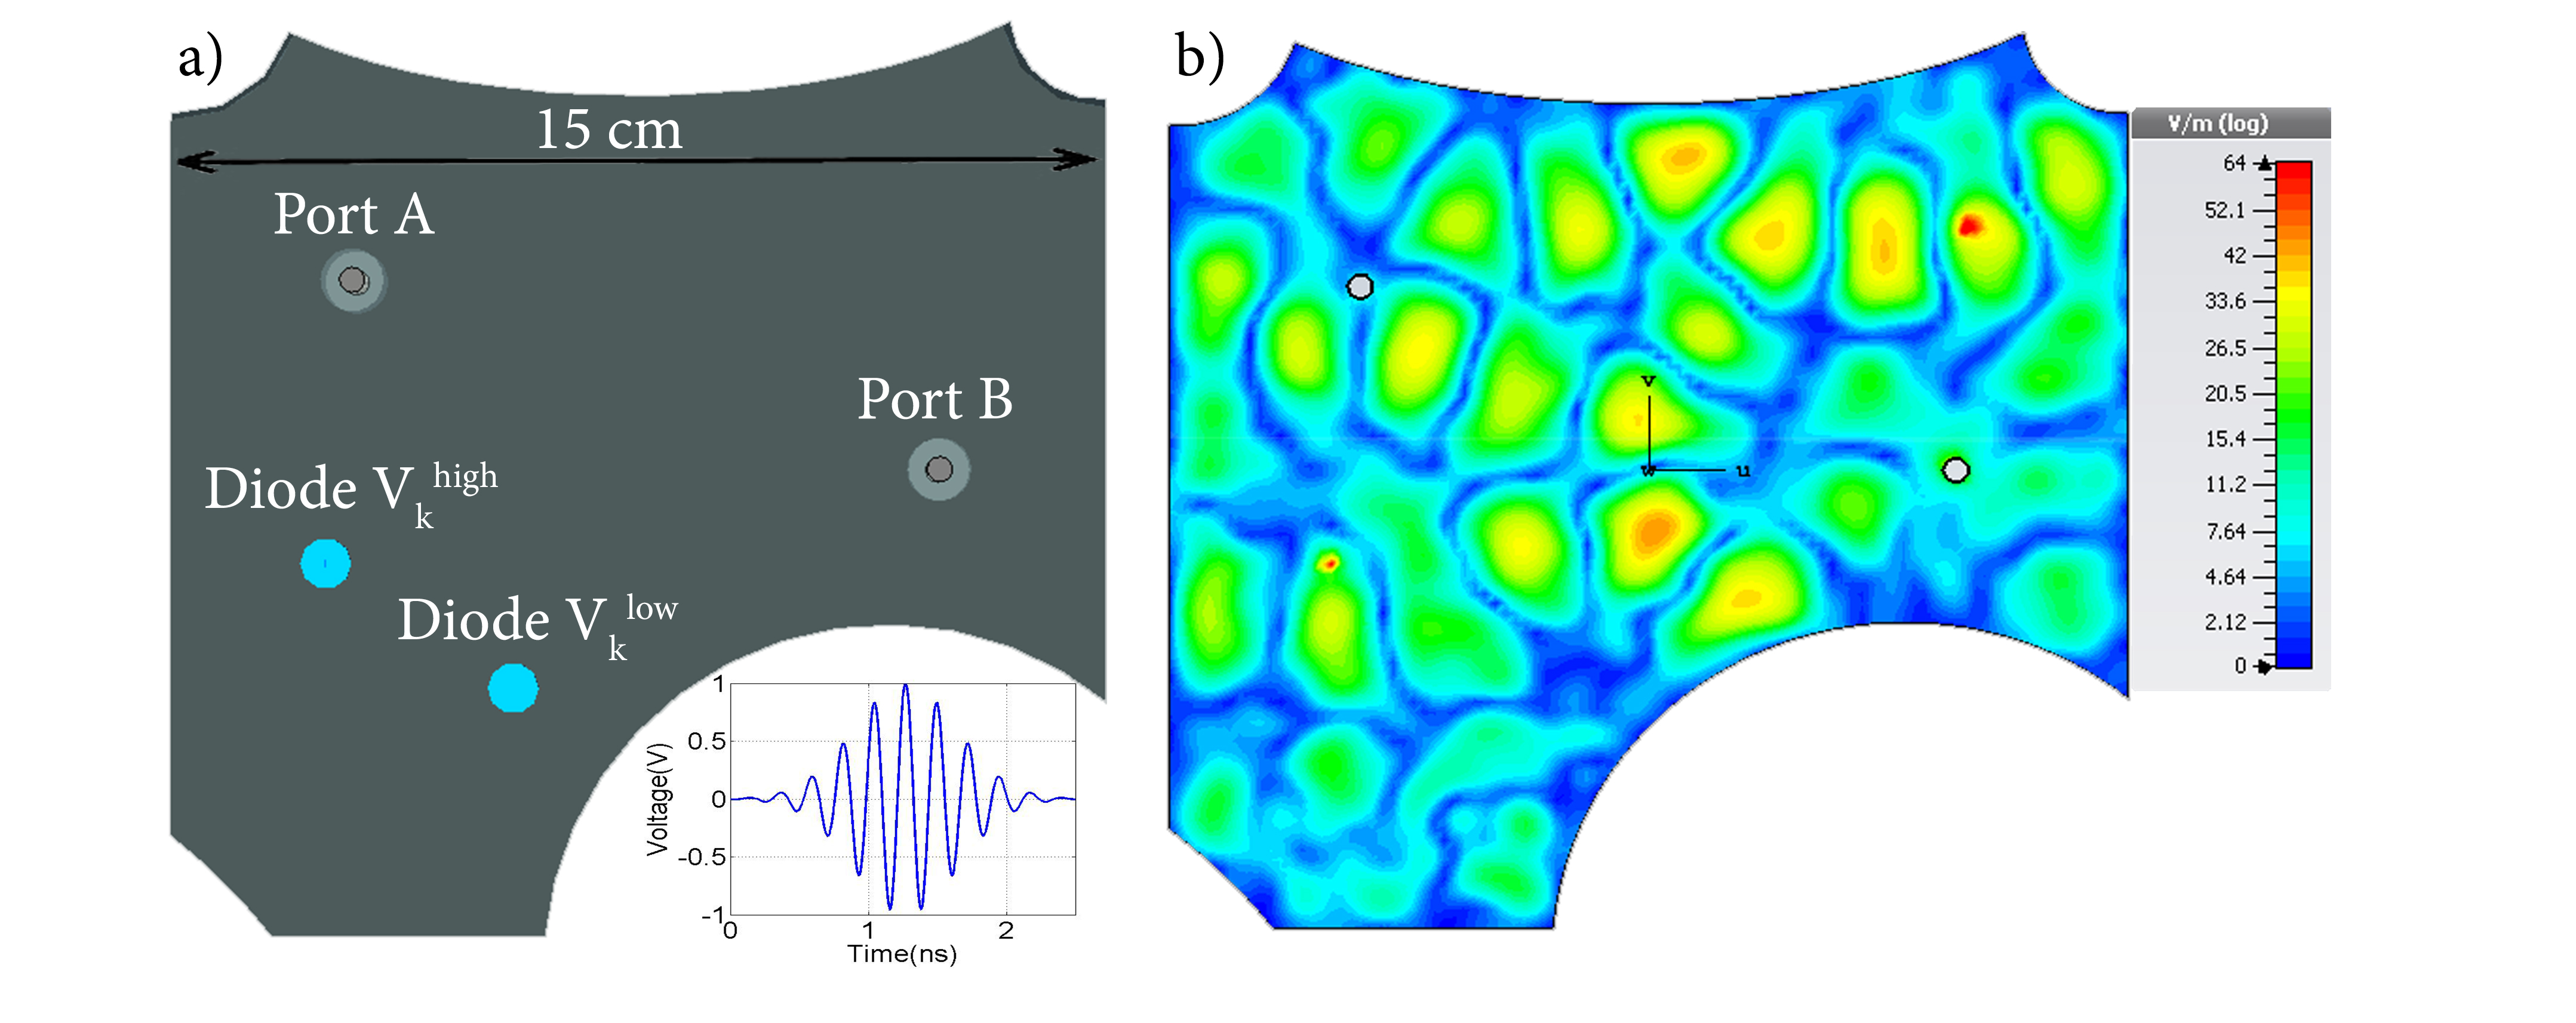
\includegraphics[width=\textwidth]{numerical/cst-box}
\caption[The Cut Box Model]{The Cut Box simulation geometry used in CST. (a) shows the location of the 2 ports (A and B), 2 diodes ($V_k^{high}, V_k^{low}$), length scale, and the lower inset shows the initial interrogation pulse. (b) shows the electric field at a point in the simulation, illustrating the limited excited mode density.}
\label{fig:numerical-cst-box}
\end{figure}

We used two Teflon-coated dipole antennas to emit and record signals~\cite{hemmady2006universal}. Two diodes are placed inside the cavity, shown by the blue circles in Figure~\ref{fig:numerical-cst-box}. A 4.4~GHz center frequency pulse with a 1.0~GHz bandwidth was chosen to minimize the reflected power and applied to antenna A. The interrogating pulse is shown as an inset in Figure~\ref{fig:numerical-cst-box}(a).

The specific frequency and bandwidth was chosen for this geometry to minimize initial wave reflection ($S_{11}$) into the enclosure. Figure~\ref{fig:numerical-s11-spectrum} shows that using a 1.0~GHz bandwidth, an optimal center frequency is 4.4~GHz. The dips in the $S_{11}$ value represent optimal frequencies to use, as a low $S_{11}$ indicates a large portion of the signal entered the cavity. The large number of peaks is indicative of the mode density of the geometry, where low frequencies are sparse given the relatively small scale of the cavity.

\begin{figure}[t]
\centering
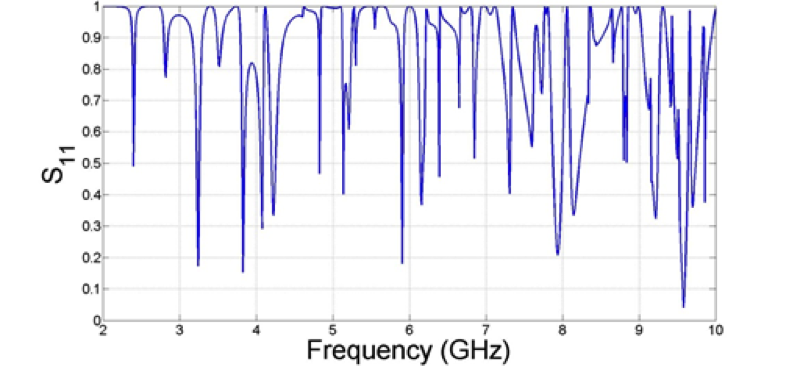
\includegraphics[width=\textwidth]{numerical/s11-spectrum}
\caption[$S_{11}$ spectrum of the Cut Box Model]{The $S_{11}$ spectrum for the Cut Box Model. We wanted to minimize $S_{11}$ for our simulation while maintaining a large bandwidth. This led to choosing a 4~GHz center frequency with a 1.0~GHz bandwidth.}
\label{fig:numerical-s11-spectrum}
\end{figure}

Using this input pulse and the pulse inversion method of sona extraction, we were able to perform NLTR in the Cut Box Model. By measuring the observed voltage and corresponding current during the time-reversed step, we measured the quasi-power over time in each diode. As shown in Figure~\ref{fig:numerical-sim-recon}, the reconstruction waveform on each diode matches the expected results for a 1-diode experiment~\cite{taddese_sensing_2010,barbieri_time_2010}.
\begin{figure}[t]
\centering
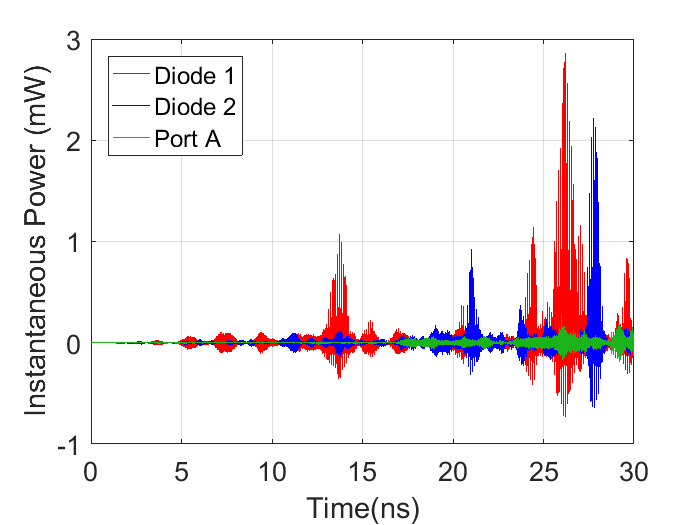
\includegraphics[width=0.75\textwidth]{numerical/sim-recon}
\caption[Simultaneous reconstructions on two diodes]{The time-reversed reconstruction on two diodes simultaneously performed inside the Cut Box geometry.}
\label{fig:numerical-sim-recon}
\end{figure}

\subsection{Discussion of Simultaneous Nonlinear Reconstructions}

This result alone signifies the generality of NLTR whereby any nonlinear object in the cavity will observe a reconstruction in the time-reversed step. In regards to a larger WPT system, one can imagine that this is particularly useful inside of a home or public area, where any device may be powered as long as it is within range of the transmitter/receiver base station. Because the process used only creates a reconstruction at the nonlinear element, it is as simple as repeating the NLTR process rapidly, creating a quasi-pulse width modulation (PWM) signal that can charge a battery. PWM is a method for controlling how active a device is by rapidly switching the device on and off. For example, a fan has different speeds because it operates 25\%, 50\%, 75\%, or 100\% of the time. Similarly, if we can reconstruct on a battery circuit every 10\% or 20\% of the time, we can effectively charge the battery. As soon as the nonlinear object leaves the enclosure, it will no longer receive power. By having a base station that can actively modulate output sona power, it would be very simple to change the amount of power transferred to each device. This dynamic power control is outside the scope of our project but represents a much later extension to this WPT system.

\subsection{Simulation of Selective Collapse of NLTR}
The logical next step is to determine how such a system would be able to determine which device should be powered. As previously shown, if nothing is done to alter the sona signals, then the sona from each nonlinear object will sum linearly and produce a reconstruction at all nonlinear objects in the time-reversed step. Given that each reconstruction sums independent of one another, we hypothesize that we should be able to eliminate the contribution of one nonlinear reconstruction to the overall set of reconstructions without altering the fidelity of any other individual reconstruction on other nonlinear elements. For example, in an enclosure with 3 diodes, if we could suppress the response of diode 2 in the time-forward step, then we would expect to only observe a reconstruction on diodes 1 and 3, creating a selective targeting method. Using Eq. 3, this would imply a weight of $x_{2} = 0$, as shown in Equation~\ref{eq:numerical-r-tot-2}.

\begin{equation}
R_{tot} = \sum_{i}R_{i}x_{i} = R_{1}x_{1} + R_{2}*0 + R_{3}x_{3} = R_{1}x_{1} + R_{3}x_{3}
\label{eq:numerical-r-tot-2}
\end{equation}

In a commercial setting, this would be an extremely useful aspect to our WPT system, as companies could require payment to use the system and would otherwise suppress the reconstruction on the user's device. The fact that the nonlinear object is passive in the environment implies that this selective targeting could even be used to ``resurrect'' a dead phone, a feature not seen on any current WPT technology on the market.

We have developed a method of performing such a targeting scheme based on the previously mentioned diode model. In the simplest case, we show that selective targeting for 2 diodes with two separate voltage knees was obtained (noted $V_k^{high}$ and $V_k^{low}$).

Recall the current response in the diode from Equation~\ref{eq:numerical-vd-gt-0}. One useful aspect to the diode definition function is that if $V < V_{k}$, then the diode has very little current response, which in turn implies a low nonlinear response. We utilize this characteristic while performing selective targeting on a low $V_{k}$ diode. Similarly, we observe that at small $V_{k}$ values, the nonlinear response is small. These two observations led to the hypothesis that nonlinear response may be maximized given an initial pulse by selecting a proper $V_{k}$ value. As shown below, Figure~\ref{fig:numerical-knee-voltages} was obtained by sweeping over many $V_{k}$ values for different initial pulse amplitudes given the same geometry and process conditions as previously stated. Given this distribution, we may target a high $V_{k}$ diode, as the nonlinear response will be stronger in the high $V_{k}$ diode than the low $V_{k}$ diode.

\begin{figure}[t]
\centering
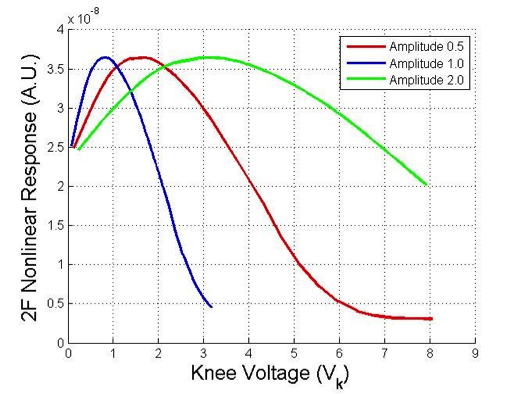
\includegraphics[width=\textwidth]{numerical/knee-voltages}
\caption[Nonlinear response due to different diode characteristics]{The nonlinear response of the diode had a clear maximum at a specific knee voltage. By using a pulse amplitude that corresponded with the specific diode knee voltage, we could selectively target diodes in CST.}
\label{fig:numerical-knee-voltages}
\end{figure}


To perform this selective targeting, we once again used the Cut Box Model. In the simplest case, we consider selective targeting of a low $V_{k} = 0.79V$ ($V_K^{low}$) diode at the exclusion of a high $V_{k} = 6.60V$ ($V_k^{high}$) diode. Given the large value of $V_k^{high}$, we expect to see no response in that diode while maintaining a reasonable nonlinear response in the $V_k^{low}$ diode. We used a pulse with amplitude $V = 1.0 V$ during the time forward step, emitted at Port A in Figure~\ref{fig:numerical-cst-box}(a). Using pulse-inversion, we extracted the nonlinear sona from the recorded signal at Port B, time-reversed the signal, and re-emitted it from Port B. Figure~\ref{fig:numerical-selective-recon-low} shows the time-reversed reconstructions on both diodes. This results in a reconstruction almost exclusively on the $V_k^{low}$ diode during the time-reversed step. The presence of three reconstructions when only one initial pulse was not alarming, as short-orbit paths between Port A, the diodes, and Port B that carry enough power to excite the diode harmonics are known to exist~\cite{hansjurgenstockmann2006}. To calculate the quality of the selective reconstruction, we determined the aspect ratio by comparing the max of $IV$ on both diodes. For this scenario, we calculate a power delivery aspect ratio of 6.35:1 for the $V_k^{low}$ diode relative to the diode with $V_k^{high}$.

\begin{figure}[t]
\centering
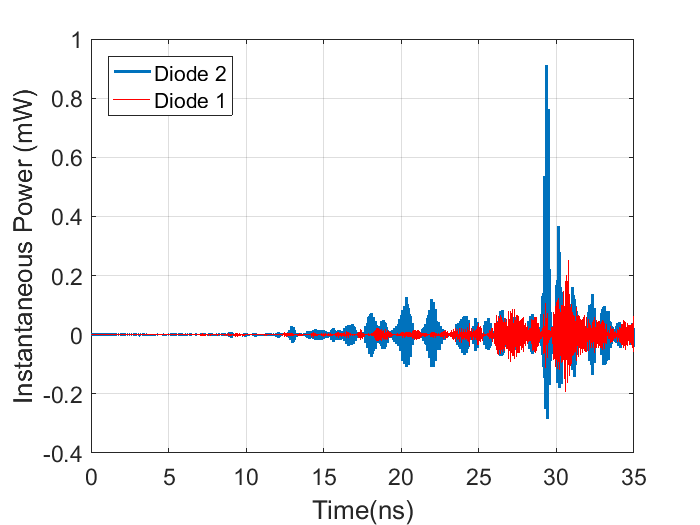
\includegraphics[width=\textwidth]{numerical/selective-recon-low}
\caption[Selective reconstruction on a $V_{k}^{low}$ diode]{Time-reversed reconstructions on the two diodes while targeting $V_{k}^{low}$. Very little signal is seen on the $V_{k}^{high}$ diode. The insert shows the details of the reconstructions between 22 and 30 ns.}
\label{fig:numerical-selective-recon-low}
\end{figure}

 The more difficult scenario was to selectively target a high $V_k$ diode at the exclusion of a low $V_k$ diode. We utilized the peak in nonlinear response as a function of knee voltage from Figure~\ref{fig:numerical-knee-voltages}. By choosing the correct pulse amplitude corresponding to a peak value that was matched to the high $V_k$ value, we expected to see the strongest nonlinear response, resulting in the largest magnitude reconstruction. In this scenario, the low $V_k$ diode still observed a reconstruction; however, it was smaller in amplitude than the high $V_k$ diode reconstruction. Given that a real system would involve a full rectification circuit in addition to the diode, the smaller amplitude reconstruction may not be able to turn on the rectifier while the high amplitude reconstruction at the high $V_k$ diode would turn on. For our simulations, we were able to model this by measuring the observed power ($I*V$) on the diode and modify the sona amplitude in order to ensure the $V_k^{high}$ diode had rectification while the $V_k^{low}$ diode did not.

\begin{figure}[t]
\centering
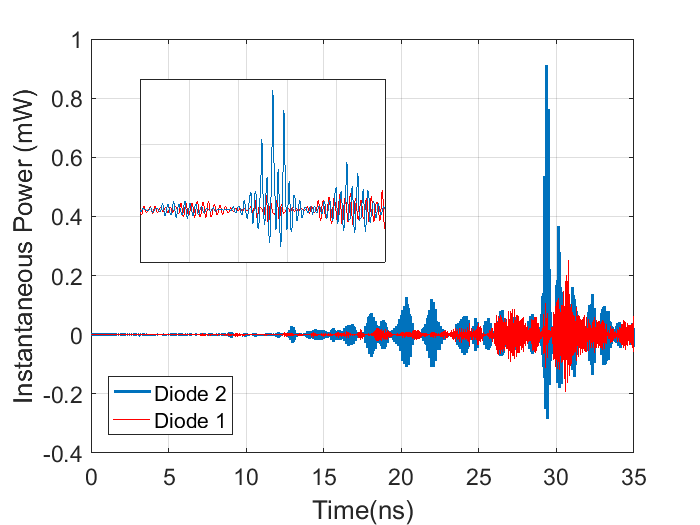
\includegraphics[width=\textwidth]{numerical/selective-recon-high}
\caption[Selective reconstruction on a $V_{k}^{high}$ diode]{Time-reversed reconstructions on the two diodes while targeting $V_{k}^{high}$. Sona amplitude modulation resulted in a clear contrast between the two signals.}
\label{fig:numerical-selective-recon-high}
\end{figure}

For this second scenario, with $V_k^{high} = 2.22V$, we once again used an amplitude $1.0 V$ pulse during the time-forward step so that we may compare the results from both scenarios equally. As shown in Figure~\ref{fig:numerical-selective-recon-high}, pulse amplitude of 1.0 has a maximum nonlinear response at $2.22V$. We chose this $V_k$ value as it gave the clearest reconstruction. Once again, we used pulse-inversion to extract the nonlinear sona. In general, this results in a larger magnitude reconstruction on $V_k^{high}$. This contrast between the $V_k^{low}$ and $V_k^{high}$ reconstructions was amplified by modulating the time-reversed sona amplitude, such that the reconstruction voltage seen at the target diode was barely larger than $V_k$ for $V_k^{high}$ and just barely smaller than $V_k$ for $V_k^{low}$. This resulted in selectively reconstructing on $V_k^{high}$ only during the time-reversed step with an aspect ratio of 3.61:1 for the $V_k^{high}$  diode relative to $V_k^{low}$, as shown in Figure~\ref{fig:numerical-selective-recon-high}.

\subsection{Discussion of Selective Nonlinear Time Reversal}

We have demonstrated a basic method for creating selective rectification using NLTR to target different nonlinear objects. This represents a stepping stone from the previously shown method of generalizing NLTR. By altering the input pulse amplitude, we were able to achieve the hypothesized nonlinear response suppression of specific nonlinear elements. This shows that the nonlinear reconstruction created on each nonlinear element is independent of one another and may be modified without impacting the other elements of the overall reconstructions. We have shown that this WPT technology would be capable of ubiquitous charging on any nonlinear device as well as selective targeting of specific devices. One may think of this as having an NLTR charger in one's home compared to having an NLTR in a business. In a domestic setting, there is very little need to restrict access to power. There are many outlets in one's home and there is no need to tell someone they are not permitted to use it. In a business however, a power outlet is not available to customers unless they pay for it. In this case, it is very useful to be able to selectively choose who may receive power. Although we have not shown a full-fledged system to do so, we have presented a foundational process that may be improved upon in order to create a successful NLTR-based WPT system.

\subsection{Simulation of Transmission Efficiency of NLTR Process}

We have so far shown that NLTR may be used in a WPT system to either power all nonlinear objects or selectively target the nonlinear objects within a relevant range. One significant question though that arises is to what efficiency are these objects powered. Surely a system that can only transfer 2\% of applied power will not be a successful WPT technology, as the consumer is paying for the luxury to not carry around a cable. If the user has to pay 50x more for the power they are very unlikely to use our system.
As previously discussed, energy losses are often difficult to calculate in real experiments due to wave reflection and other systematic sources of error. However, by simulating the NLTR process, we are able to observe approximate transfer efficiency. In CST, we are able to track input power and power loss via wave reflection, absorption in both lumped elements and environment materials, and radiation loss at other ports. One drawback to using the built-in CST power tracking is that everything is recorded in the frequency domain rather than time domain. For example, a typical power spectrum from a time-reversed step of a 2-diode NLTR simulation is shown in Figure~\ref{fig:numerical-power-spectrum}. As we are interested in overall power input compared to overall power output, we used this data along with Equation~\ref{eq:numerical-transfer-efficiency} to compute the efficiency of transfer in our simulations.

\begin{equation}
e = \frac{\sum_{i}P_{i(diode)}(f)}{\sum_{i}P_{i(input)}(f)} \cdot 100
\label{eq:numerical-transfer-efficiency}
\end{equation}

\begin{figure}[t]
\centering
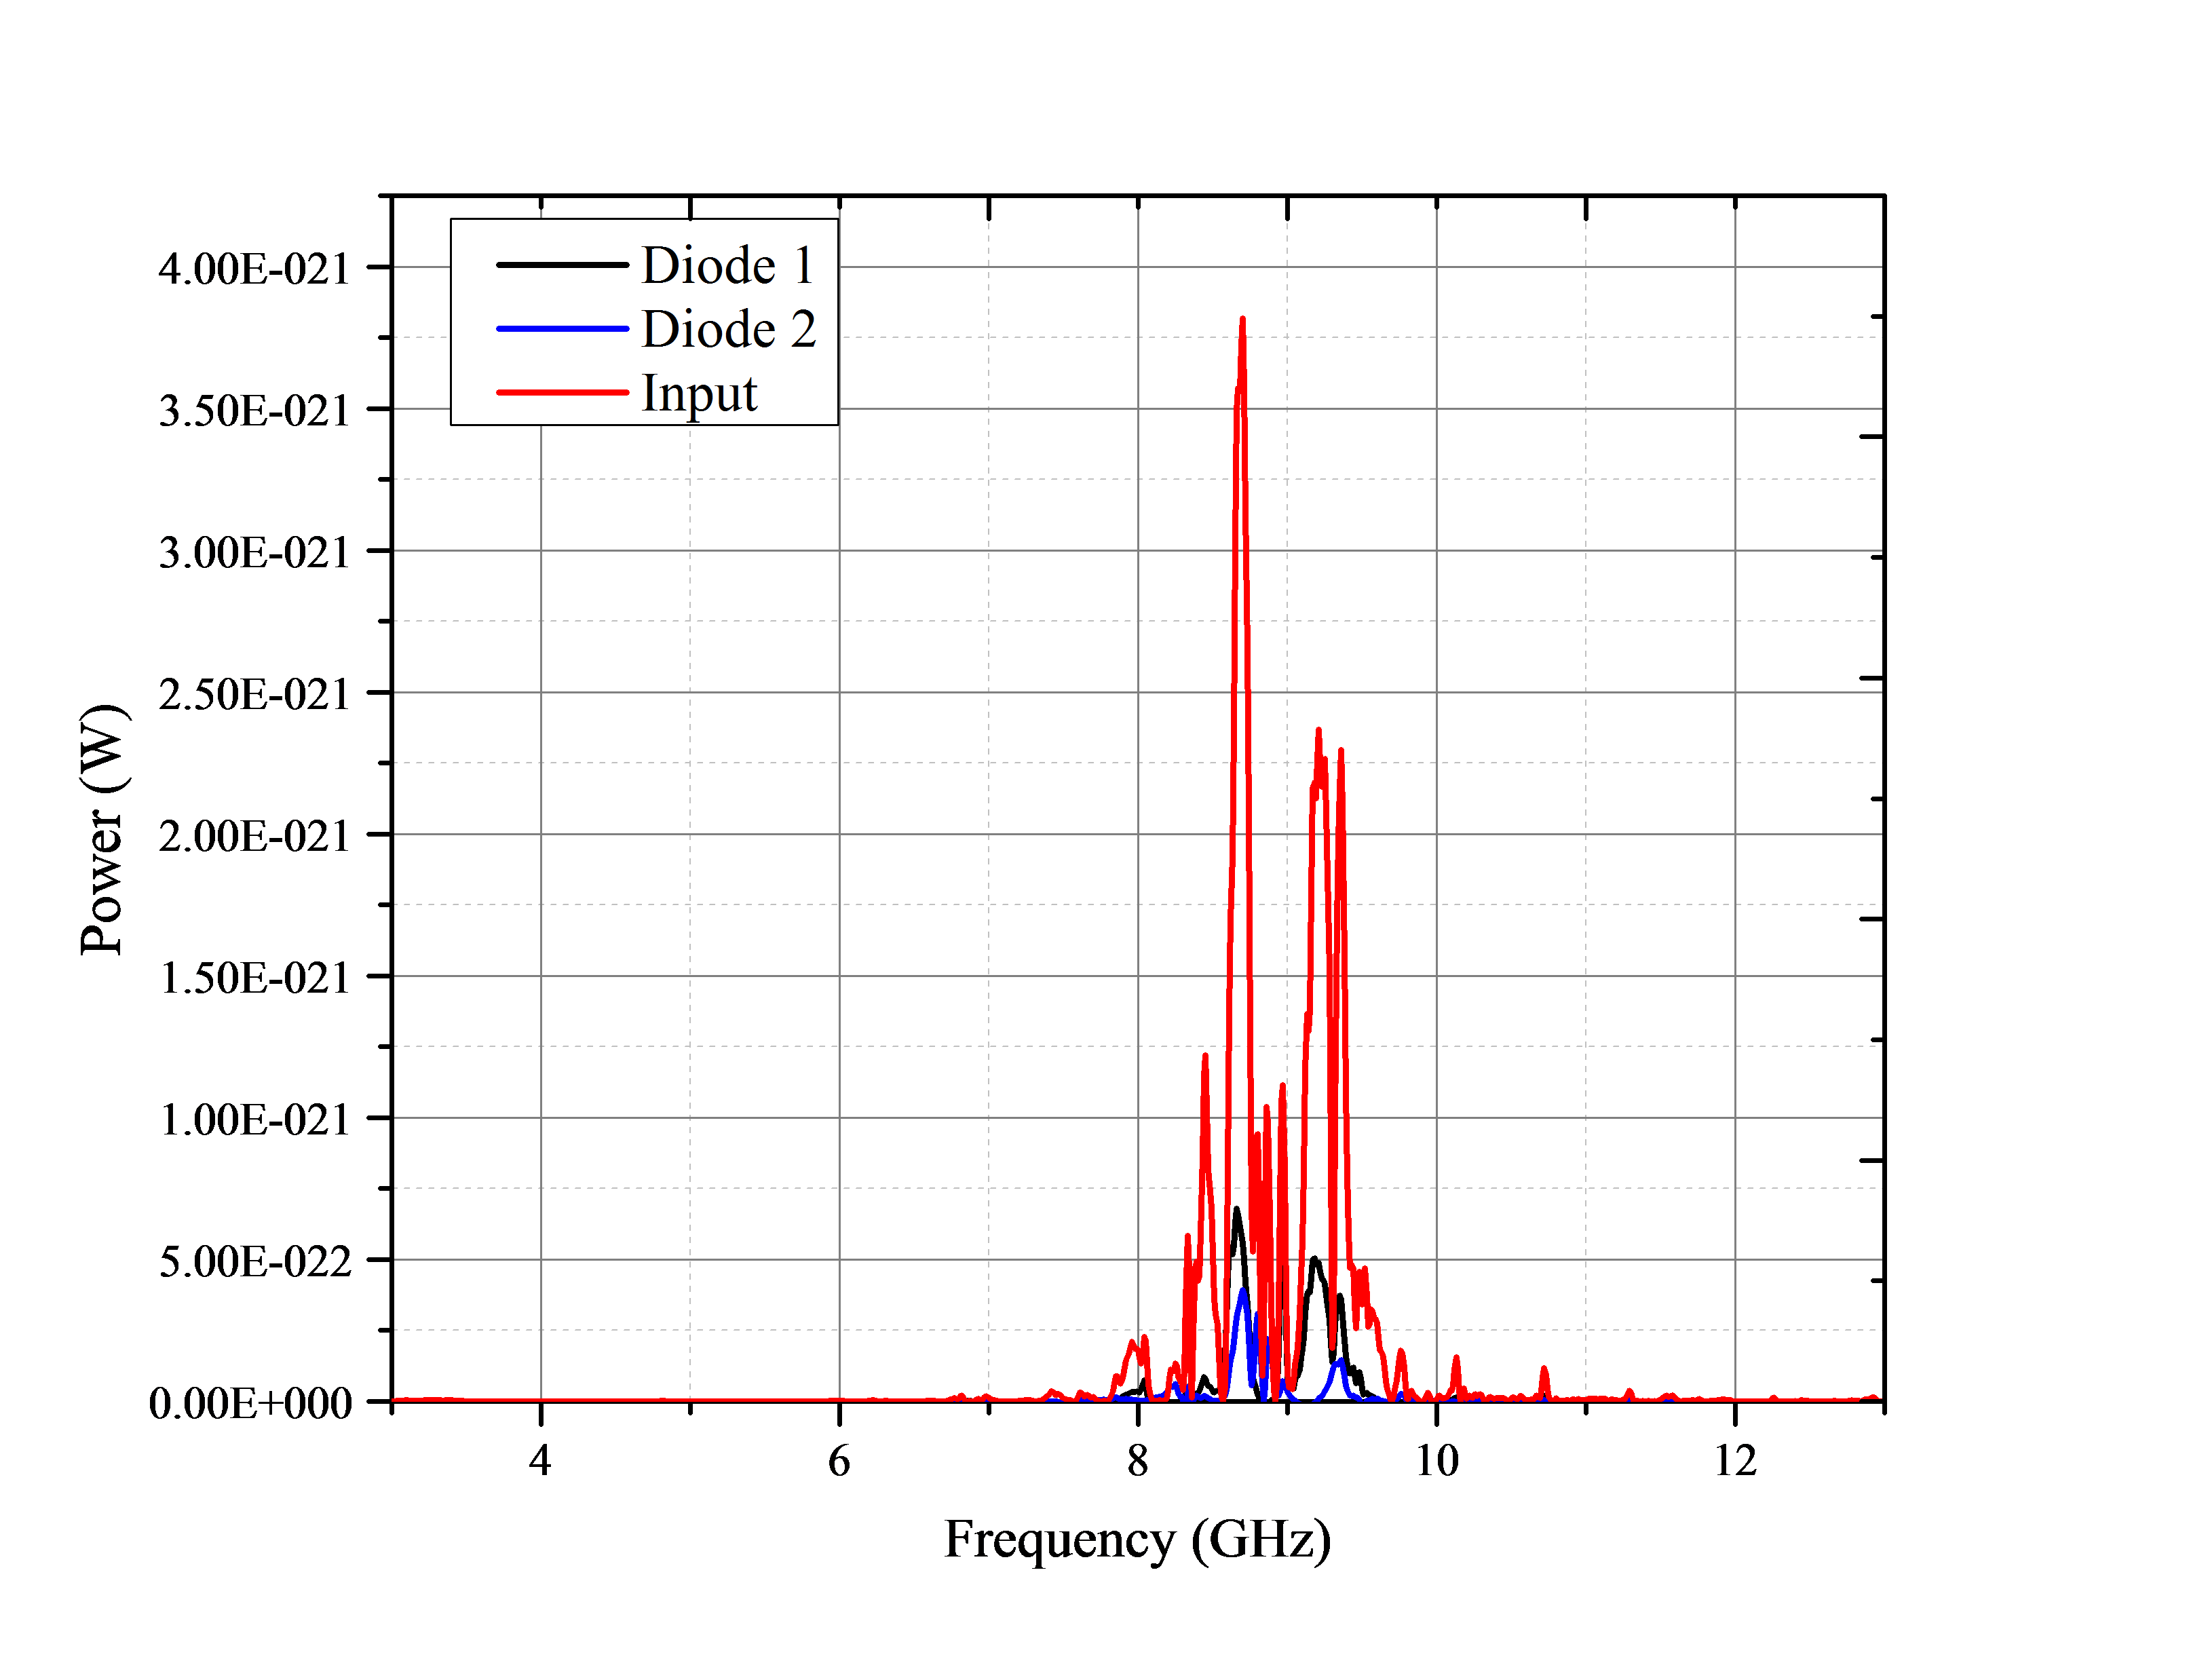
\includegraphics[width=\textwidth]{numerical/power-spectrum}
\caption[Transfer efficiency for a two-diode simultaneous reconstruction]{A typical power spectrum obtained in the time-reversed step (reconstruction). The power that enters the diodes only represents a portion of the overall power input in the simulation.}
\label{fig:numerical-power-spectrum}
\end{figure}

The above data was taken from a simulation in the Cut Box model for the previously discussed two-diode simultaneous reconstruction. For this simulation, we found that $18.6$\% and $7.3$\% of power were transferred from the nonlinear sona to diodes 1 and 2, respectively.  This provides a promising outlook.

Our next question was whether or not these transfer efficiencies were a function of distance between transmitter port, diode, and receiver port. We found that using similar diode positions as previously stated resulted in transmission values around the \numrange{7}{18}\% shown above. We decided to introduce a new model with a much larger length scale, called the Room Model shown in Figure~\ref{fig:numerical-room-model}.

\begin{figure}[t]
\centering
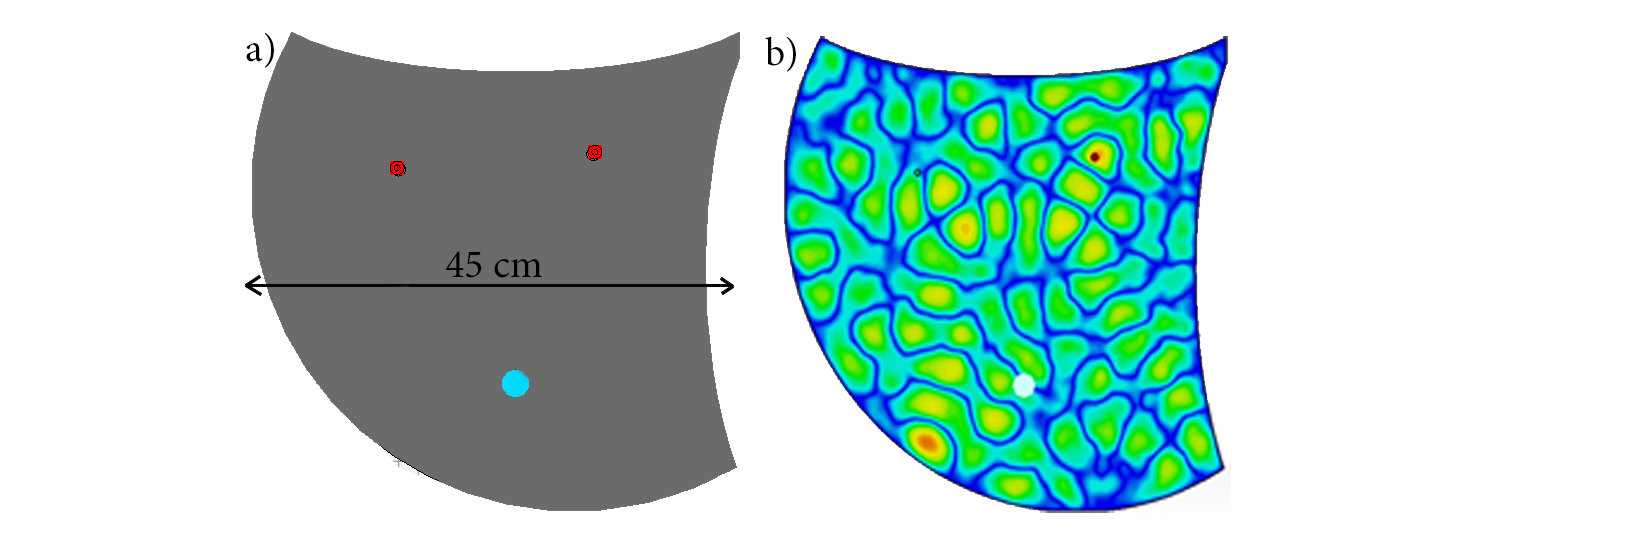
\includegraphics[width=0.85\textwidth]{numerical/room-model-a}
\caption[The Room Model]{(a) illustrates the geometry of the Room Model and (b)
shows the mode density of the space.}
\label{fig:numerical-room-model}
\end{figure}


We chose to use a 45cm x 45cm x 0.76 cm initial box to simulate a large geometry while still maintaining a quasi-2D cavity. The 45~cm length scale was used, as any larger simulation ran out of memory prior to completion.  Due to the length of simulation and decreased nonlinear signal strength, this model was unable to be used for further efficiency calculations. From Figure~\ref{fig:numerical-room-model}, the distances in the simulation are much larger than the Cut Box and may be used in the future to determine whether transmission efficiency of NLTR is dependent on distance between transmitter, nonlinear object, and receiver ports.

\section{Conclusion}
\label{sec:numerical-conclusion}

Using CST, we have successfully demonstrated our 3 goals: (1) simultaneous reconstructions on multiple nonlinear objects (2) selective reconstructions between multiple nonlinear objects and (3) calculation of a baseline transmission efficiency of NLTR. For simultaneous and selective targeting, we provide a basic framework to perform these processes using numerical simulations; however, these processes are still yet to be performed in real-world experimentation. We believe that this illustrates a foundational work for future experiments to demonstrate the feasibility of these features in a new WPT technology. Additional research must be done in order to characterize the ceiling on transmission efficiency if NLTR is to be applied to a future WPT technology.

\chapter{Development of a Super Rectenna}
\label{ch:rectenna}
\section{Goals of Rectenna}
\label{sec:rectenna-goals}

One of the main components of any WPT system is its rectifier, as it performs the crucial step of capturing the broadcast energy and transforming it into a usable form. To accomplish this, a rectenna, a dual-purpose device that combines an antenna and a rectifier, is necessary. The antenna picks up the oscillating AC signal received from the transmitter, the rectifier converts the signal to relatively stable DC power, and this usable power is passed to an arbitrary load.

In addition to standard rectification, the rectenna must serve as a passive nonlinear element. In NLTR, a nonlinear element is required to produce harmonics from the initial interrogation pulse broadcast by the transmitter. This goal is secondary to the main purpose of rectification.

The rectenna was designed to satisfy the following parameters. First, the rectenna must operate efficiently at the high frequency (\numrange{1}{10}~GHz) required for efficient NLTR. Additionally, losses due to reflection and parasitic effects within the antenna should be minimized. Finally, to fulfill the role of a nonlinear element, the rectenna should generate distinguishable harmonics strong enough for the purposes of NLTR.

In short, to rectify and generate harmonics for NLTR, the rectenna must be capable of not only efficient rectification at high frequencies, but also production of strong harmonics for NLTR.

\section{Diode Selection and Testing}
\label{sec:rectenna-diode}

The diode is the most important single component to consider for the rectenna, as it is the main rectifying component. Careful consideration of its characteristics is vital. The switching frequency, forward voltage drop, and impedance of the diode are of particular importance to the desired goal of efficient rectification.

For the rectenna in our design to perform efficiently, the diode must satisfy several requirements:

The diode must maintain rectification functionality at a transmission frequency of \numrange{1}{10}~GHz. This requirement severely limits the possible choices for the rectenna diode. The frequency of a diode is inversely related to its reverse-recovery time ($t_{rr}$), the fastest time the diode can switch from forward to reverse bias~\cite{an1012-TRR}. In traditional P-N junction diodes, minimum $t_{rr}$ is on the order of tens to thousands of nanoseconds, even for fast diodes~\cite{davis2011schottky}. In a high frequency circuit, a P-N diode would be no different than a short circuit, and no rectification would occur.

The diode must have the lowest forward voltage drop possible. The voltage drop represents the reverse bias that remains when the diode works in the forward direction, and can be a significant contributor to power loss. The team's experimental WPT capabilities are limited to fairly low voltage microwave signals (.5 V to 1 V signal amplitude), which makes forward voltage drop especially important.

Finally, impedances should be minimized. All diodes have intrinsic impedances such as parasitic capacitance and resistance. Impedances contribute to losses during rectification, and minimizing these losses would increase the efficiency of rectification.

Considering these factors, a Schottky barrier diode was chosen for the rectenna. Unlike P-N junction diodes, Schottky diodes have extremely low $t_{rr}$ and low forward voltage~\cite{davis2011schottky}.  Schottky diodes do have a lower maximum reverse voltage rating, higher reverse leakage current, and higher cost than P-N diodes. However, these are relatively minor issues in our application. A Schottky \texttt{MA4E1317} diode was used as the rectifying diode. The diode parameters from the manufacturer's datasheet are shown in Table~\ref{tab:rectenna-datasheet}.

\def\arraystretch{2}
\begin{table}[h]
\centering
\begin{tabular}{|c|c|c|c|c|c|}
\hline
\textbf{Test Conditions} & \textbf{Symbol} & \textbf{Units} & \textbf{Min.} & \textbf{Typ.} & \textbf{Max.} \\ \hline
Junction Capacitance at 0 V at 1 MHz & Cj & pF & - & .020 & - \\ \hline
Total Capacitance at 0 V at 1 MHz & Ct & pF & .030 & .045 & .060 \\ \hline
Junction Capacitance Difference & DCj & pF & - & - & - \\ \hline
Series Resistance at +10 $mA$ & Rs & $\Omega$ & - & 4 & 7 \\ \hline
Forward Voltage at +1 $mA$ & $Vf_1$ & V & .60 & .70 & .80 \\ \hline
Forward Voltage Difference at +1 $mA$ & DVf & V & - & - & - \\ \hline
Reverse Breakdown Voltage at $-10 \mu A$ & Vbr & V & 4.5 & 7 & - \\ \hline
SSB Noise Figure & NF & dB & - & $6.5^4$ & - \\ \hline
\end{tabular}
\caption[Datasheet for diode used in rectenna construction]{Datasheet for the M/A-Com \texttt{MA4E1317} Schottky diode~\cite{ma4e1317-datasheet}.}
\label{tab:rectenna-datasheet}
\end{table}

The \texttt{MA4E1317} has low total capacitance (.045~pF) and series resistance (4~$\Omega$), minimizing parasitic losses. The datasheet also cites an operating frequency of up to 80 GHz for this diode, more than sufficient for our purposes. The forward voltage cited to be around .7~V, a typical value for most diodes~\cite{ma4e1317-datasheet}. A lower forward voltage would be desirable, and in considering future improvements to the system, this is definitely a point to consider.

\section{Antenna Design}
\label{sec:rectenna-antenna}

A printed circuit board (PCB) half-wave dipole was chosen as the antenna for the system. The copper trace patterned on the FR-4 substrate acts as the antenna. The \texttt{MA4E1317} is a flip-chip device, and is only suitable for mounting on a PCB. The design and specific parameters of the antenna is based on the dual frequency WPT rectenna in~\cite{suh2002high}, but has been modified for our implementation. The design of the rectenna is shown in Figure~\ref{fig:rectenna-design}.


\begin{figure}[]
    \centering
    \begin{subfigure}{.85\textwidth}
        \centering
        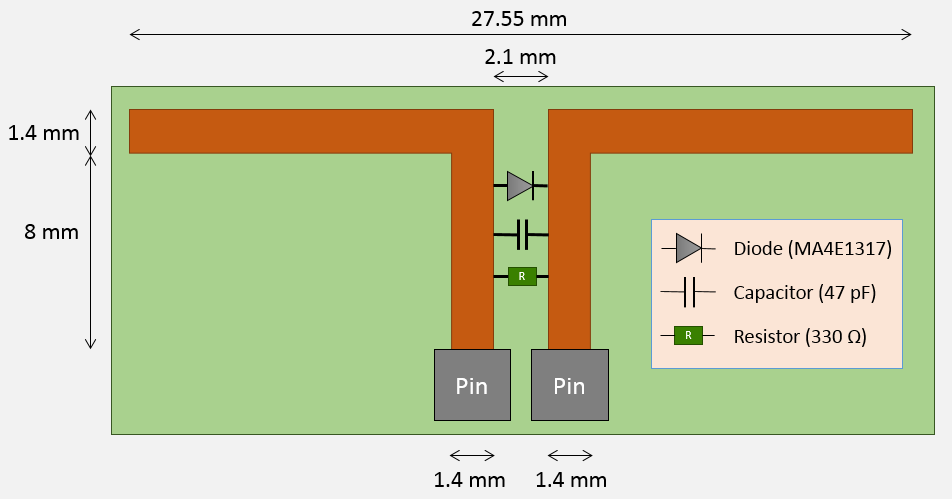
\includegraphics[width=1.0\linewidth]{rectenna/rectenna-design}
        \caption[Rectenna schematica]{A schematic of the PCB rectenna design and component specifications.}
    \end{subfigure}
		\par\bigskip
    \begin{subfigure}{.85\textwidth}
        \centering
        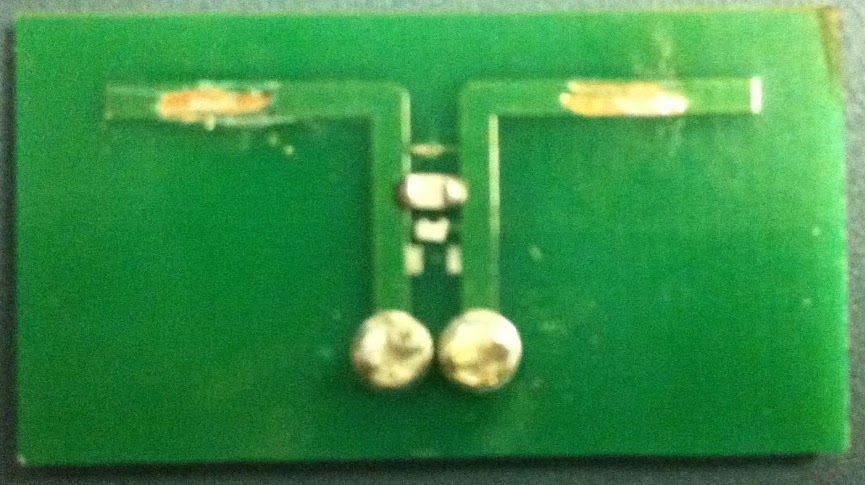
\includegraphics[width=1.0\linewidth]{rectenna/rectenna-photo}
        \caption[Assembled rectenna photo]{Image of the assembled rectenna}
    \end{subfigure}
    \caption[Rectenna design]{Rectenna design}
    \label{fig:rectenna-design}
\end{figure}

The rectenna is composed of three surface-mount components. The \texttt{MA4E1317} diode acts as the rectification and harmonic generation components. A 47~pF high-frequency ceramic capacitor acts as a low-pass filter, blocking microwave signal from reaching the load. Finally, a 330~$\Omega$ resistor is used as a load for experimental purposes. Output pins also attached for measurement purposes. The antenna is designed for operation at 5.45~GHz, so the length of the dipole is 27.55~mm, half the free-space wavelength of the incident wave.

The topology of the diode was chosen to maximize rectification efficiency. The Schottky diode is positioned shunt to the feed-in lines of the rectenna. This topology was chosen instead of a voltage doubler (a two diode configuration) because of its inherently higher power efficiency. However, if higher voltage levels are necessary for a load device, the voltage doubler would be a better choice~\cite{boaventura2015boosting}. Both options should be considered for future iterations of our design.

One important distinction for this rectenna design is the lack of band-pass filtering for higher-order harmonics. This feature is common in most rectennas, but is deliberately left out to allow the harmonic response of the diode to escape through the dipole.

It is worth noting, however, that we did not attempt impedance matching between the antenna and the rectifier components. This is an important point to consider for future work, as proper matching of the components should significantly improve the efficiency of rectification.

\section{Rectenna Testing}
\label{sec:rectenna-testing}

To thoroughly test the rectenna, distinct tests were run in order to verify both its rectification and harmonic generation capabilities. We examined a range of frequencies for all tests to isolate peak performance.

\subsection{DC Power Characterization}

To determine the overall rectification efficiency, a second antenna was used to broadcast energy to the rectenna. A 17~dBm~CW signal was generated from the PSG and broadcast through a monopole antenna. The rectenna was then positioned parallel to the broadcast antenna, at a distance of 2~cm, and the average DC voltage and power was measured over the load resistor. The test was repeated over a range of broadcast frequencies from 1~to~7~GHz. The setup is shown in Figure~\ref{fig:rectenna-test-1-setup} and the results are shown in Figure~\ref{fig:rectenna-test-1-voltage}.


\begin{figure}[]
    \centering
    \begin{subfigure}{.85\textwidth}
        \centering
        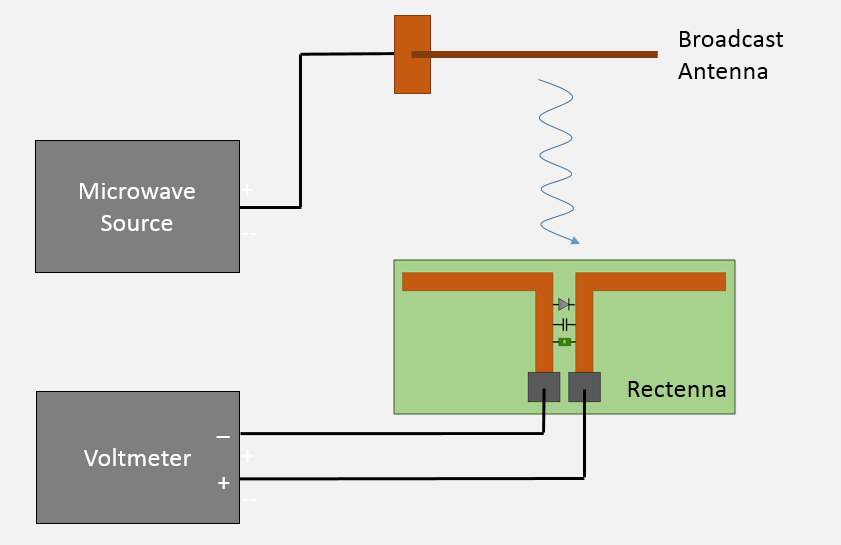
\includegraphics[width=1.0\linewidth]{rectenna/test-1-setup}
        \caption{Experimental setup for rectification testing}
        \label{fig:rectenna-test-1-setup}
    \end{subfigure}
		\par\bigskip
    \begin{subfigure}{.85\textwidth}
        \centering
        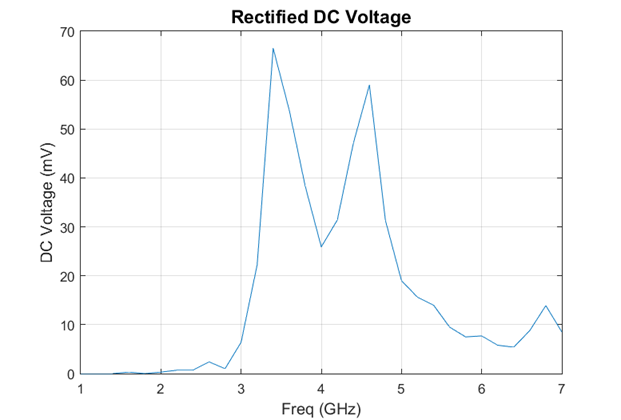
\includegraphics[width=1.0\linewidth]{rectenna/test-1-voltage}
        \caption{Average DC voltage measured from the voltmeter in the setup on the left for a range (1-7~GHz) of frequency inputs.}
        \label{fig:rectenna-test-1-voltage}
    \end{subfigure}
    \caption[Rectenna Rectification]{Rectenna rectification testing}
    \label{fig:rectenna-test-1}
\end{figure}

Rectification was most pronounced in the 3-5~GHz frequency band. Rectified voltage is highest at 3.4~GHz and 4.6~GHz, with DC voltage levels of 66.5~mV and 59.0~mV respectively. Unfortunately, DC voltage results of higher frequencies were unreliable and erratic given the measurement techniques, and accurate data could not be collected.

Given the resistive load of 330~$\Omega$, rectified DC power can be calculated from the voltage above. Using DC voltage ($V$) and load resistance ($R$), the average DC power ($P_{dc}$) was calculated using Equation ~\ref{eq:dc_power}:

\begin{equation}
P_{dc} = \frac{V^2}{R}
\label{eq:dc_power}
\end{equation}

A plot of the resulting average DC power delivered to the load as a function of frequency is shown in Figure~\ref{fig:rectenna-test-1-power}.

\begin{figure}[]
\centering
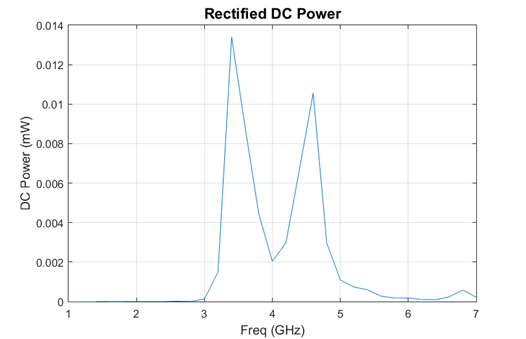
\includegraphics[width=0.85\textwidth]{rectenna/test-1-power}
    \caption[Rectified DC power]{Average rectified DC power calculated from DC voltage using the relation: $P = \frac{V^2}{R}$}
    \label{fig:rectenna-test-1-power}
\end{figure}


Considering the input power of 17~dBm (around 50.12~mW), the wall-to-load efficiency of the experiment is extremely low for all frequencies. These losses can come from a number of sources, including bad coupling between the broadcast antenna and rectenna, reflection from broadcast antenna, losses in coaxial connections between components, and power radiated away from the rectenna, among others. However, the inherent losses of the experimental setup are not relevant to the overall efficiency of the system; for this, the DC rectification result must be compared to only to power accepted by the antenna.

To establish rectification efficiency, AC power tests were conducted on a bare dipole antenna with no diode, resistor, or capacitor. The results of this test establish the overall power accepted by the rectenna, representing the peak power available for rectification. These results are directly comparable to the previous DC power results.

The setup of the AC power experiment was similar to the DC power experiment, with the exception of two key differences: the voltmeter was replaced by a \texttt{DSO91304A} oscilloscope, and the rectenna was replaced by the bare dipole antenna. In the absence of the 330~$\Omega$ load resistor on the rectenna, the 50~$\Omega$ input impedance of the oscilloscope~\cite{DSO91304A-manual} was used as the load.

Using AC voltage amplitude ($V_{max}$) and load resistance ($R$), the accepted AC power ($P_{ac}$) was calculated using Equation ~\ref{eq:ac_power}:

\begin{equation}
P_{ac} = \frac{V_{max}^2}{2R}
\label{eq:ac_power}
\end{equation}

The setup and results of the test are shown below in Figures~\ref{fig:rectenna-test-2-setup}~and~\ref{fig:rectenna-test-2-power}, respectively.

\begin{figure}[]
    \centering
    \begin{subfigure}{.85\textwidth}
        \centering
        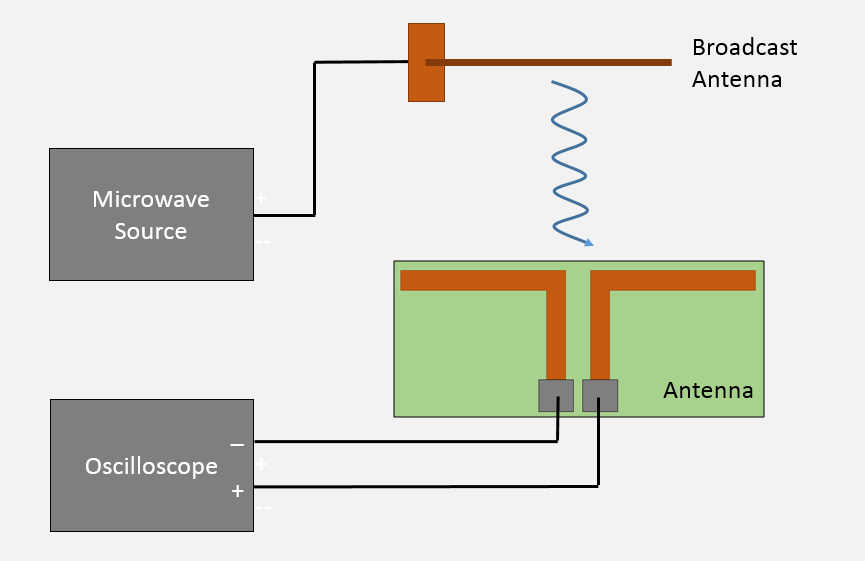
\includegraphics[width=1.0\linewidth]{rectenna/test-2-setup}
        \caption{Experimental setup for measuring accepted AC power}
        \label{fig:rectenna-test-2-setup}
    \end{subfigure}
		\par\bigskip
    \begin{subfigure}{.85\textwidth}
        \centering
        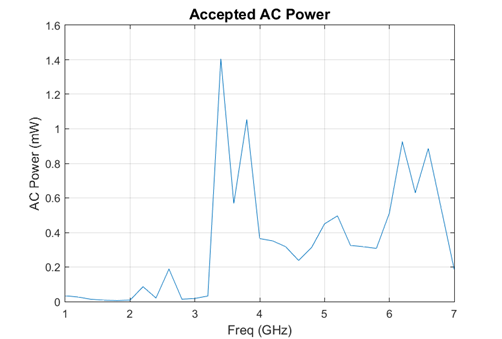
\includegraphics[width=1.0\linewidth]{rectenna/test-2-power}
        \caption[Accepted AC power]{Accepted AC power, used to establish a baseline for efficiency calculation, calculated using the relation $P = \frac{V_{max}^2}{2R}$.}
        \label{fig:rectenna-test-2-power}
    \end{subfigure}
    \caption[Measuring accepted AC power]{Measuring accepted AC power}
    \label{fig:rectenna-test-2}
\end{figure}

Assuming that the transfer function between the antennas doesn't change between the AC and DC tests, these results allow the rectification efficiency to be calculated. The efficiency ($E$) in this case is the ratio of the rectified DC power ($P_{dc}$) to the total accepted AC power ($P_{dc}$), as in Equation ~\ref{eq:rec_eff}:

\begin{equation}
E = \frac{P_{dc}}{P_{ac}}
\label{eq:rec_eff}
\end{equation}

Figure~\ref{fig:rectenna-efficiency} shows the efficiency calculated this way, across the range of frequencies tested.

\begin{figure}[]
\centering
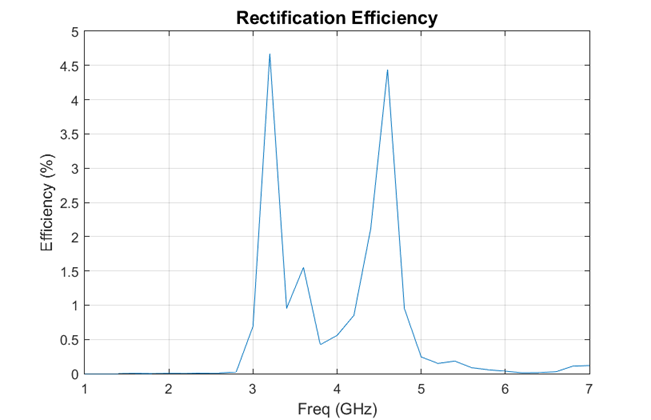
\includegraphics[width=0.85\textwidth]{rectenna/efficiency}
    \caption[Rectification efficiency]{Rectification efficiency, calculated using accepted AC power as a baseline. Calculated using the ratio of rectified DC power to accepted AC power.}
    \label{fig:rectenna-efficiency}
\end{figure}

Analysis of the graph shows the same peak rectification efficiencies at 3.2~GHz and 4.6~GHz, with 4.7\% and 4.4\% respectively. This rather low efficiency is expected given the lack of optimization and impedance matching in the rectenna. However, this result clearly demonstrates rectification of microwave power to DC power.

\subsection{Harmonic Generation}

Harmonic generation was tested by measuring second harmonic power reflected from the rectenna. A microwave source produced  a 10~dBm~CW signal, which was broadcast from a bare antenna of the same length as the rectenna. The rectenna, positioned around 1 mm away in the same orientation as the broadcast antenna, should passively generate second harmonics from this fundamental signal. These second harmonic reflections were collected by the bare antenna, passing through a directional coupler and into a spectrum analyzer for measurement. The test setup and results for this experiment are shown in Figure~\ref{fig:rectenna-test-3-setup}.

\begin{figure}[]
\centering
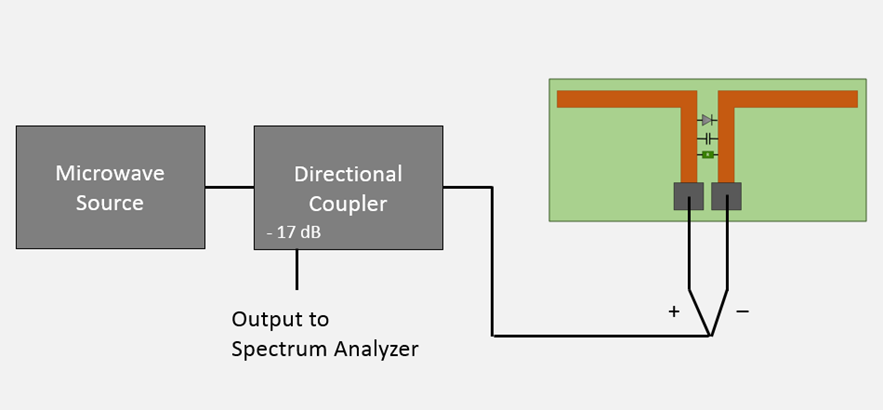
\includegraphics[width=0.85\textwidth]{rectenna/test-3-setup}
\caption{Experimental setup for harmonic generation testing.}
\label{fig:rectenna-test-3-setup}
\end{figure}

As seen in the experimental setup, harmonic responses from microwave source were filtered out with a combination of high and low pass filters. A distinct 2nd harmonic was found at 2.45~GHz at -150~dBm, distinctly higher than to the noise level power of -161~dBm. Bandwidth restrictions of filtering components prevented analysis of a full frequency spectrum, and thus, 2.45~GHz is the only frequency we were able to probe for harmonics. Even so, this result does demonstrate the harmonic generation capabilities of the rectenna.

\section{Discussion}
\label{sec:rectenna-discussion}

The intent of the rectenna was twofold. The rectenna was designed to rectify RF signals (\numrange{1}{10}~GHz) and generate higher-order harmonics. Both of these qualities are needed for the creation of an NLTR rectifier. The current experiments establish a baseline for rectification and harmonic generation that can be used for future designs.

The current experiments establish a baseline for rectification and harmonic generation that can be used for future designs. The current design has made no steps toward the impedance matching of the antenna to the components. This is likely a major source of power lost by the system for rectification, and should be a top priority to consider in subsequent designs. While rectenna designs vary based on specific application, it is not uncommon for a rectenna to achieve 70-90+\% efficiency~\cite{class-e, novel-multi-coil}. Clearly, there are many improvements that need to be made to bring our ~5\% efficiency to these much higher values.
Future rectenna design may benefit from physically splitting the base signal from its harmonic so that the two signals may have dedicated circuitry for each goal. The base signal would be optimized for harmonic generation while the 2f harmonic input would be optimized for rectification. One such method is using a multiplexer to split incident signal into a 1f and 2f signal [ku-band]. This system would not suffer parasitic losses due to frequency mismatch between the 1f and 2f circuitry.


Our design of a dual-purpose rectenna has satisfied our initial goals, and is a first step towards a functioning NLTR based WPT system.  It is able to receive the initial interrogation pulse and generate a 2nd harmonic response. It is also able to receive the high power pulse and rectify the signal, providing the load device with DC power. Due to the nature of NLTR, the receiving devices do not require power to facilitate either process. After considerable optimization and miniaturization, the rectenna would be used as a general-purpose receiver for the electronics we want to power.

\chapter{Conclusion}

\label{ch:conclusion}

\todo{Need to fill this out}

\section{Future Work}

\todo{Consider looking at last paragraph or two from Scott’s section.}

Thanks to the generosity of Dr. Anlage and the UMD CNAM, Team TESLA had access to several state-of-the-art measuring and testing devices. Researching alongside graduate students associated with the CNAM, TESLA explored TR WPT primarily through the behavior of reconstruction, including how sonas can be manipulated to change reconstruction parameters.  Experiments including minimum TR cycle time, overlapping sonas, and reconstruction profile characterization have added to the literature surrounding practical TR, but gaps in knowledge continue to remain.  Many of these gaps we have identified are due to limitations in TESLA's technical expertise and lack of  access to proper equipment.  As a result of these shortcomings, we suggest areas of further research that could yield fruitful results with a dedicated and pioneering team, including what experiments could address these gaps.  It is our hope that our research will lay groundwork for further explorations of how TR can be applied to practical WPT.

\subsection{Equipment Limitations}

The aluminum echoic chamber used in tests (the Gigabox), and the equipment used to transmit and measure EM waves within this chamber, were from previous experiments on TR done by graduate students under Dr. Anlage.  These resources allowed TESLA a great deal of freedom in designing experiments.  However, monetary and physical resources of the team limited the purchase of additional equipment, and this in turn restricted the experiments that could be done.

The Gigabox was designed to be an ideal environment to study TR from a signal processing point of view. However, the Gigabox is not easily modified from this purpose. A Gigabox with interchangeable panels will allow for the creation of testing environments of differing absorption, translucence, and geometry. Fine control of these parameters will aid the development of a model for the effects of environment on the power losses of TR WPT. The lack of this model for transmission efficiency is one of the greatest hurdles towards designing a TR WPT system.

Better tools can help the team revisit previously unsuccessful experiments. Early in TESLA’s research the team investigated how antenna design and form could relate to TR convergence.  This path yielded inconclusive results for a variety of reasons. Due to lack of resources and inexperience, the team approached antenna design and testing using a “rapid prototyping” plan that resulted in inconsistent designs. Higher quality fabrication techniques, coupled with prototyping in simulations, could have improved this aspect of research.  We suggest that future research in TR antenna optimization should focus on the creation of nonlinearly reflective antennas useful in NLTR.  These antennas will allow experiments on TR WPT with multiple receivers, a topic which may offer significant advances in the field.

\subsection{Technical Inexperience}

TESLA's research into TR was very much a learning experience.  The team began its research with little to no experience with TR, or with academic research as a whole.  As a result, many of the team's early research results should be reconsidered or revisited. There are other areas that the team did not investigate at all, and which now are obvious areas of research.

TESLA’s experimentation focused significantly on the relationship between sona and reconstruction, and there are more areas within this topic that should be revisited in greater detail.  TESLA performed several early experiments on partial sonas to see how they relate to reconstruction quality.  However, the team prioritized completion of other tests at the time, as there was an unclear sense of practical application or benefit by continuing.  In retrospect, these tests may be useful in relating the sona to the environmental characteristics and should be considered in more detail.

Future researchers may want to consider the quality of reconstructions created with partial sonas.  This research should also give a better quantification of what “reconstruction quality” means for arbitrary reconstruction waveforms. It could be beneficial to find methods of relating sona length and general shape to geometric factors of the environment. Understanding this relationship can allow the optimization of a TR WPT system for a given environment. The reverse is also true; some modifications to the transmission environment may help improve efficiency.

Finally, the effect of iterative time reversal on reconstruction was ignored in TESLA's tests.  The team suggests that it should be considered in future experimentation. Iterative time reversal mirrors are common in the literature for signal focusing [CITE HERE], and there is reason to believe that iteration will also improve EM TR WPT.  Iteration may have significant effects on transfer efficiency and spatial profile.  However, iteration is also based off of the idea of a stationary target, and may not work well for moving targets.  This tradeoff, once understood, will greatly help optimize the system.

\subsection{Summary}

Outline: (I'm writing below this outline and I have to say I don't like all of the items on it -Tim)
	What discoveries or accomplishments have been made:
Overlapping Reconstructions
Ability to produce continual reconstructions on a stationary target
Simultaneous reconstructions {linear TR}?
Spatial Profile
Description of localization of reconstructions on a stationary targets
Moving Reconstructions
Demonstrate capability to follow moving receiver based on spatial profile of reconstruction on a quasi-stationary receiver.
Selective Targeting
Ability to selectively target diodes by exploiting their separate nonlinear characteristics.
Simultaneous reconstructions (non via overlapping sonas {nonlinear TR})?
ferromagnetic nanorods
Identifying potential nonlinear elements to be used in NLTR
Properties of nanorod harmonic generation: amplification, suppression, and/or absence of nonlinear response
Rectenna

We hypothesized that overlapping reconsturctions by overlaying sonas could result in more effective power transmitted per duty cycle. Our experiments seemed to support this in that the number of reconstructions in the cycle could be increased while maintaining their characteristic shape. However, our lab equipment attempted to scale each arbitrary waveform we broadcast to the same total output power. This prevented us from definitively finding a relationship between the number of reconstructions and the power received by the target.

As part of investigating TR's applicability to WPT, the team wanted to map how broad and how strong the excitation from the collapsing wavefront was around a target antenna. An understanding of this would be useful to engineers attempting to integrate a TR WPT system into any larger system. Reconstruction were mapped at a variety of frequencies, and the width of this spatial profile was found to be directly related to the wavelength.

The spatial profiling told us that the region of excitation around a target could be relatively broad compared to the size of our antenna. Next, we wanted to see whether we could take advantage of this by repeatedly re-targeting an antenna as it began to move out of the region of greater power. In this way, we hoped it would be possible for a TR WPT system to maintain steady power delivery to the target. Our results appeared to show that it should be, though we were somewhat limited by the time our TRM took to aquire a new sona and retarget the antenna.

In summary, several technical accomplishments have been made to assist


%% Glossary
\renewcommand{\baselinestretch}{1}
\small\normalsize
\printglossary
\clearpage

\printglossary[type=\acronymtype]
\clearpage
\newpage


%% Bibliography
%% This defines the bibliography file (main.bib) and the bibliography style.
%% If you want to create a bibliography file by hand, change the contents of
%% this file to a `thebibliography' environment.  For more information 
%% see section 4.3 of the LaTeX manual.
\begin{singlespace}
\bibliography{main}
\bibliographystyle{plain}
\end{singlespace}


\end{document}

%%%%%%%%%%%%%%%%%%%%%%%%%%%%%%%%%%%%%%%%%%%%%%%%%%%%%%%%%%%%%%%%%%%%%%%%%%%%%%%
